\documentclass[12pt,a4paper]{article}
\usepackage[T1]{fontenc} %Cyrillic and English
\usepackage[utf8]{inputenc}
\usepackage[english]{babel} 
\usepackage{amsmath}
\usepackage{amsthm}


%Fonts
\usepackage{mathrsfs}
%\usepackage[cal=esstix, frak=esstix]{mathalfa}
\usepackage{amsfonts} %Always load this after mathalfa
\usepackage{amssymb} %Always load this after mathalfa

%Misc
\usepackage{graphicx}
\usepackage{mathtools}
\usepackage{cleveref}
\usepackage[top=0.5cm,left=2cm,right=2cm,bottom=1.5cm]{geometry}
\usepackage{subcaption}
%\usepackage{bbm}
\usepackage{float} 

%Bibliography
%Change sorting to other options. 
%The parameter giveninits shortens the authors first names
\usepackage[bibencoding=auto,backend=biber,sorting=none,giveninits=true]{biblatex}
%Separator between the authors should be a comma 
\renewcommand{\finalnamedelim}{\addcomma\space}

\newtheorem{theorem}{Theorem}
\newtheorem{lemma}[theorem]{Lemma}
\newtheorem{corollary}[theorem]{Corollary}
\newtheorem{defn}[theorem]{Definition}
\newtheorem{example}[theorem]{Example}
\newtheorem{remark}[theorem]{Remark}

%Additional Math commands and shortcuts
\newcommand\mynewcommand[1]{\let#1\relax\newcommand#1}
\mynewcommand{\f}[1]{\mathfrak{#1}}
\mynewcommand{\c}[1]{\mathcal{#1}}
\mynewcommand{\b}[1]{\mathbb{#1}}
\mynewcommand{\bf}[1]{\bm{#1}}
\mynewcommand{\s}[1]{\mathscr{#1}}
\mynewcommand{\intg}[3]{\int_{#1} #2 \,\text{d}#3}
\mynewcommand{\intb}[4]{\int_{#1}^{#2} #3 \,\text{d}#4}
\DeclarePairedDelimiter{\norm}{\lVert}{\rVert}
\DeclarePairedDelimiter{\abs}{\lvert}{\rvert}

\DeclareMathOperator{\sign}{sign}
\DeclareMathOperator{\argmin}{argmin}
\DeclareMathOperator{\diag}{diag}
\DeclareMathOperator{\AC}{AC}

\newcommand{\mat}[1]{\left(\begin{matrix}#1\end{matrix}\right)}
\newcommand{\smat}[1]{\left(\begin{smallmatrix}#1\end{smallmatrix}\right)}

\begin{document}
	%Title
	\begin{center}
		\Large \textsc{Adaptive Control}
	\end{center}

	Thilo Herold \hfill Simon Land \hfill Andrey Kharitenko \hfill Problem Set 01

	\section*{Problem 1}
	
	\subsection*{Mathematically rigorous proof of stability and tracking}
	
	In the next we want to deal with discontinuous reference signals $r(t)$.
	For $c \in [0,\infty]$ let
	\begin{align*}
		\AC[0,c)
		= \{f:[0,c) \to \b{R} \mid f \text{ absolutely continuous on every compact }[a,b] \subseteq [0,c)\}
	\end{align*}
	and $L^\infty[0,\infty)$ denotes the space of essentially bounded functions on $[0,\infty)$.
	All derivatives $f'(t)$ of $f \in \AC[0,\infty)$ are meant to be defined for almost all $t \in [0,\infty)$.
	Since our ODE-solutions will only be differentiable almost everywhere, we need the following well-known existence theorem:
	\begin{theorem}[Caratheodory existence theorem]
		Let $F:\b{R}^n \times [0,\infty) \to \b{R}^n$ be a function so that $F(\cdot,t)$ is continuous for all $t \in [0,\infty)$, $F(y,\cdot)$ is measurable for all $y \in \b{R}^n$. 
		If for all compact $K \subseteq \b{R}^n \times [0,\infty)$, there exists some function $m_K \in L^1[0,\infty)$ such that $\norm{F(y,t)} \leq m_K(t)$ for all $(y,t) \in K$, then for any $y_0\in \b{R}^n$ the initial value problem
		\begin{align*}
			y'(t) = F(y(t),t)\,, \quad
			y(0) = y_0 
		\end{align*}
		has a local (absolutely continuous) solution $y$ on some (maximal) interval of existence $[0,t_+)$ and such that $\norm{y(t)} \to \infty$ as $t \nearrow t_+$ if $t_+ < \infty$.
	\end{theorem}
	\begin{proof}[Proof]
		See any non-introductory book on ODEs, e.g. Theory of Ordinary Differential Equations by E. A. Coddington and N. Levinson.
	\end{proof}
	\begin{theorem}[Stability and tracking]
		Let $G$ be a plant given as the solution of
		\begin{align*}
			\dot{x}_p(t) = a_p x_p(t) + k_p u(t) + \alpha_p^\top f(x_p(t))\,, \quad 
			x_p(0) = x_{p,0}
		\end{align*}
		where 
		$x_p, u \in \AC[0,\infty)$, $f\in C(\b{R},\b{R}^l)$ and $a_p,k_p \in \b{R}$, $k_p \neq 0$ and $\alpha_p \in \b{R}^l$. 
		Suppose that $M$ is a model plant given by $\dot{x}_m(t) = a_m x_m(t) + k_m r(t)$, $x_m(0) = x_{m,0}$, where $x_m\in \AC[0,\infty)$, $r \in L^\infty[0,\infty)$ and $a_m,k_m \in \b{R}$, $a_m < 0$. 
		Set 
		\begin{align*}
			\theta_a^* = \frac{a_m-a_p}{k_p}\,, \quad 
			k^* = \frac{k_m}{k_p}\,, \quad 
			\alpha^* = -\frac{1}{k_p}\alpha_p\,.
		\end{align*}
		Let $\Gamma \in \b{R}^{(l+2) \times (l+2)}$ be such that $\Gamma > 0$ and let $e(t) = x_p(t) - x_m(t)$ and 
		\begin{align*}
			\phi:[0,\infty) \to \b{R}^{l+2}\,, t \mapsto (r(t), x_p(t), f(x_p(t))^\top)^\top\,.
		\end{align*}
		If we close the loop by setting $u(t) = \Theta(t)^\top \phi(t)$, where $\Theta(t) = -\sign(k_p)\intb{0}{t}{e(s)\Gamma\phi(s)}{s} + \Theta_0$, then the closed loop solution $x_p$ exists, is bounded and $\lim_{t \to \infty} e(t) = 0$.
	\end{theorem}

	\begin{proof}
		We must first show that the closed loop system is well-defined and admits solution functions $x_p$, $x_m$ and $\Theta$ which do \textbf{not blow up} in finite time.
		Formally closing the loop with $u(t) = \Theta(t)^\top \phi(t)$ yields the following ODE-system:
		\begin{align*}
			\dot{x}_p(t) &= a_p x_p(t) + k_p (r(t), x_p(t), f(x_p(t))^\top) \Theta(t)  + \alpha_p^\top f(x_p(t)) \\
			\dot{x}_m(t) &= a_m x_m(t) + k_m r(t) \\
			\dot{\Theta}(t) &= -\sign(k_p) (x_p(t)-x_m(t)) \Gamma (r(t), x_p(t), f(x_p(t))^\top)^\top
		\end{align*}
		with initial value $(x_p(0),x_m(0),\Theta(0)) = (x_{p,0},x_{m,0},\Theta_0)$.
		The middle ODE is independent of the other two and it can be easily shown that its unique solution is given by 
		\begin{align*}
			x_m(t) = e^{a_m t} x_{m,0} + \intb{0}{t}{e^{a_m(t-s)}k_m r(s)}{s}\,,
		\end{align*}
		which is bounded, as $a_m < 0$ and $r \in L^\infty[0,\infty)$.
		Eliminating the middle equation thus yields
		\begin{align*}
				\dot{x}_p(t) &= a_p x_p(t) + k_p (r(t), x_p(t), f(x_p(t))^\top) \Theta(t)  + \alpha_p^\top f(x_p(t)) \\
				\dot{\Theta}(t) &= -\sign(k_p) (x_p(t)-x_m(t)) \Gamma (r(t), x_p(t), f(x_p(t))^\top)^\top\,,
		\end{align*}
		with initial value $(x_p(0),\Theta(0)) = (x_{p,0},\Theta_0)$.
		This can be rewritten into 
		\begin{align*}
			 y' = \mat{\dot{x_p}\\ \dot{\Theta}} = F\left(\mat{x_p\\ \Theta},t\right) = F(y,t)
		\end{align*}
		where 
		\begin{align*}
			F\left(\mat{x_p \\ \Theta},t\right)
			= \mat{a_px_p + k_p (r(t), x_p, f(x_p)^\top) \Theta  + \alpha_p^\top f(x_p) \\ -\sign(k_p) (x_p-x_m(t)) \Gamma (r(t), x_p, f(x_p)^\top)^\top}\,.
		\end{align*}
		We need to show that the initial value problem $y'(t) = F(y,t)$, $y(0) = y_0$ admits a global solution (that is bounded on every finite interval).
		We will first show that there exists a local solution by means of the Caratheodory existence theorem.
		First note that $F(y,\cdot)$ is measurable for all $y$ (as $r$ is measurable) and $F(\cdot,t)$ is continuous, as $f$ is continuous and all operations defining $F$ are continuous.
		Now, if $K \subseteq \b{R}^{l+3} \times [0,\infty)$ is compact, then there is some $C>0$ such that if $\smat{x_p \\ \Theta} \in K$ then $\abs{x_p} < C$, $\norm{\Theta} < C$ and $\norm{f(x_p)} < C$, as $f$ is continuous.
		By direct computation for all $\smat{x_p \\ \Theta} \in K$
		\begin{gather*}
			\norm*{F\left(\mat{x_p \\ \Theta},t\right)} \\
			\leq \abs{a_px_p + k_p (r(t), x_p, f(x_p)^\top) \Theta  + \alpha_p^\top f(x_p)} + \abs{(x_p-x_m(t)) \Gamma (r(t), x_p, f(x_p)^\top)^\top} \\
			\leq \abs{a_p}\abs{x_p} + \abs{k_p}\norm*{\smat{r(t)\\ x_p \\ f(x_p)}}\norm{\Theta} + \norm{\alpha_p}\norm{f(x_p)} + \abs{x_p-x_m(t)}\norm{\Gamma}\norm*{\smat{r(t)\\ x_p \\ f(x_p)}} \\
			\leq C\abs{a_p}+\abs{k_p} (\abs{r(t)}+2C)C + C\norm{\alpha} + (C+\abs{x_m(t)})\norm{\Gamma}(\abs{r(t)}+2C) =: m_K(t)\,,
		\end{gather*}
		where we have used the fact that $\norm{z} \leq \sum_{i=1}^n \abs{z_i}$ for $z \in \b{R}^n$. 
		Now, $m_A(t)$ is bounded and supported on a compact set, i.e. $m_K \in L^1[0,\infty)$.
		Hence the Caratheodory existence theorem is applicable and we get that there exists some solution $y = \smat{x_p\\\Theta}$ of the IVP defined on some maximal interval of existence $[0,t_+)$.
		In the next we show that $t_+ = \infty$.
		First obverse that (this was shown rigorously in the lecture)
		\begin{align}
			\dot{e}(t) = a_m e(t) + \frac{k_m}{k^*} = \tilde{\Theta}(t)^\top \phi(t)
			\quad \text{for almost all } t \in [0,t_+)\,.
			\label{eq:errorDynamics}
		\end{align}
		where $\tilde{\Theta}(t) = \Theta(t) - (k^*,\theta_a^*,(\alpha^*)^\top)^\top$ is the parameter error.
		
		Now, define a function $V$ by
		\begin{align*}
			V(e,\tilde{\Theta})
			= \frac{1}{2}e^2 + \frac{1}{2}\abs{k_p} \tilde{\Theta}^\top \Gamma^{-1} \tilde{\Theta}\,, \quad 
			e \in \b{R}\,, \tilde{\Theta} \in \b{R}^{l+2}\,.
		\end{align*}
		Let $W(t) = V(e(t),\tilde{\Theta}(t))$, then $W \in \AC[0,t_+)$.
		Then, as was shown again rigorously in the lecture, we have
		\begin{align*}
		    W'(t)
			= \frac{d}{dt} W(t)
			= a_m e(t)^2 \quad 
			\text{for almost all } t \in [0,t_+)\,.
		\end{align*}
		Note that $W' \in \AC[0,t_+)$, that $W(t) \geq 0$ and $W'(t) \leq 0$ for almost all $t \in [0,t_+)$ and that hence $\lim_{t \nearrow t_+} W(t) = \inf_{t \in [0,t_+)} W(t)$ exists.
		Thus $e(t)$, $\Theta(t)$ (and $x_p(t) = e(t)+x_m(t)$) must be bounded as $t \nearrow t_+$, since otherwise $W(t)$ would be unbounded as $t \nearrow t_+$, which would contradict the fact that $\lim_{t \nearrow t_+} W(t)$ exists. 
		Hence we have shown that $t_+ = \infty$ and that $x_p$ and $\Theta$ exist on all of $[0,\infty)$.
		Now we will show that they are bounded on $[0,\infty)$ and that $\lim_{t \to \infty} e(t) = 0$.
		By doing the same calculations we see that (\ref{eq:errorDynamics}), $W(t) \geq 0$ and $W'(t) \leq 0$ hold for almost all $t \in [0,\infty)$ and that therefore $\lim_{t \to \infty} W(t) = \inf_{t \in [0,\infty)} W(t)$ exists. 
		By the Lyapunov stability theorem, the functions $e$ and $\tilde{\Theta}$ are bounded\footnote{This can also be seen directly, since if $e$ or $\tilde{\Theta}$ were unbounded, so would be $W$, which contradicts the fact that $W$ has a limit for $t \to \infty$.}.
		Then $\Theta$ and $x_p = e+x_m$ are bounded and as $f$ is continuous, also $f(x_p)$.
		But in this case $\phi$ and $u = \Theta^\top \phi$ are bounded.
		As $\dot{x_p} = a_p x_p + k_p u + \alpha_p f(x_p)$ and $\dot{x_m} = a_m x_m + k_m r$, we have that $\dot{e} = \dot{x_p} - \dot{x_m}$ is bounded and hence there is some $C > 0$ such that  
		\begin{align*}
			\abs*{W''(t)} 
			= \abs{2 a_m e(t) \dot{e}(t)}
			\leq C \quad 
			\text{for all } t \in [0,\infty)\,.
		\end{align*} 
		Then the function $W'$ is Lipschitz-continuous, as
		\begin{align*}
			\abs{W'(t_1)-W'(t_2)} \leq \sup_{t \in [t_1,t_2]} \abs{W''(t)} \abs{t_1-t_2} \leq C\abs{t_1-t_2}\,,
		\end{align*}
		by the mean value theorem. 
		This means that in particular $W'$ is uniformly continuous on $[0,\infty)$.
		As $\lim_{t \to \infty} W(t)$ exists, we get by Barbalat's lemma $\lim_{t \to \infty} W'(t) = 0$, which implies that
		\begin{align*}
			\lim_{t \to \infty} e(t) = \lim_{t \to \infty} \sqrt{\frac{W'(t)}{a_m}} = 0\,.
		\end{align*}  
	\end{proof}

	\subsection*{Linear plant}
	
	We have $a_p = 1$, $k_p = 3$, $a_m = -4$, $k_m = 4$. 
	Hence the true control parameters are given by 
	\begin{align*}
		\theta_a^* = \frac{a_m-a_p}{k_p} = -\frac{5}{3}\,, \quad 
		k^* = \frac{k_m}{k_p} = \frac{4}{3}\,.
	\end{align*}
	Here are our simulation results for $T_{\text{max}} = 10s$:

		\begin{figure}[H]
			\centering
			\begin{subfigure}{.45\textwidth}
				\centering
				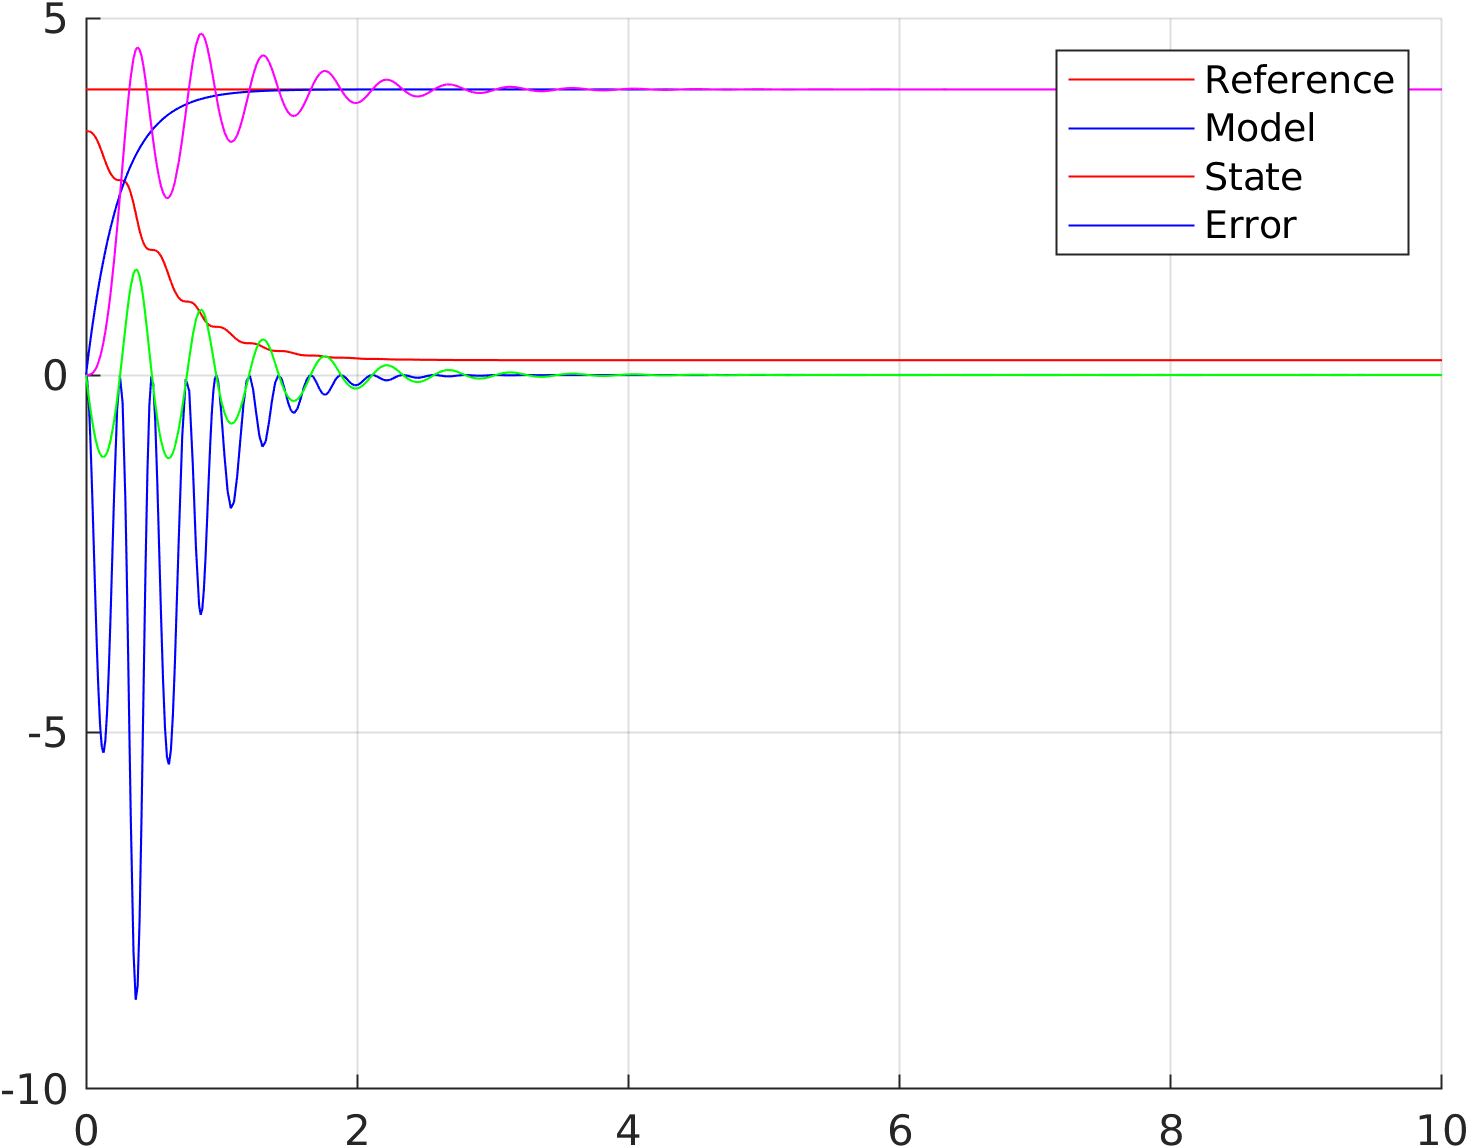
\includegraphics[width=1\textwidth]{Graphics/LinearState1.png}
			\end{subfigure}%
			\begin{subfigure}{.45\textwidth}
				\centering
				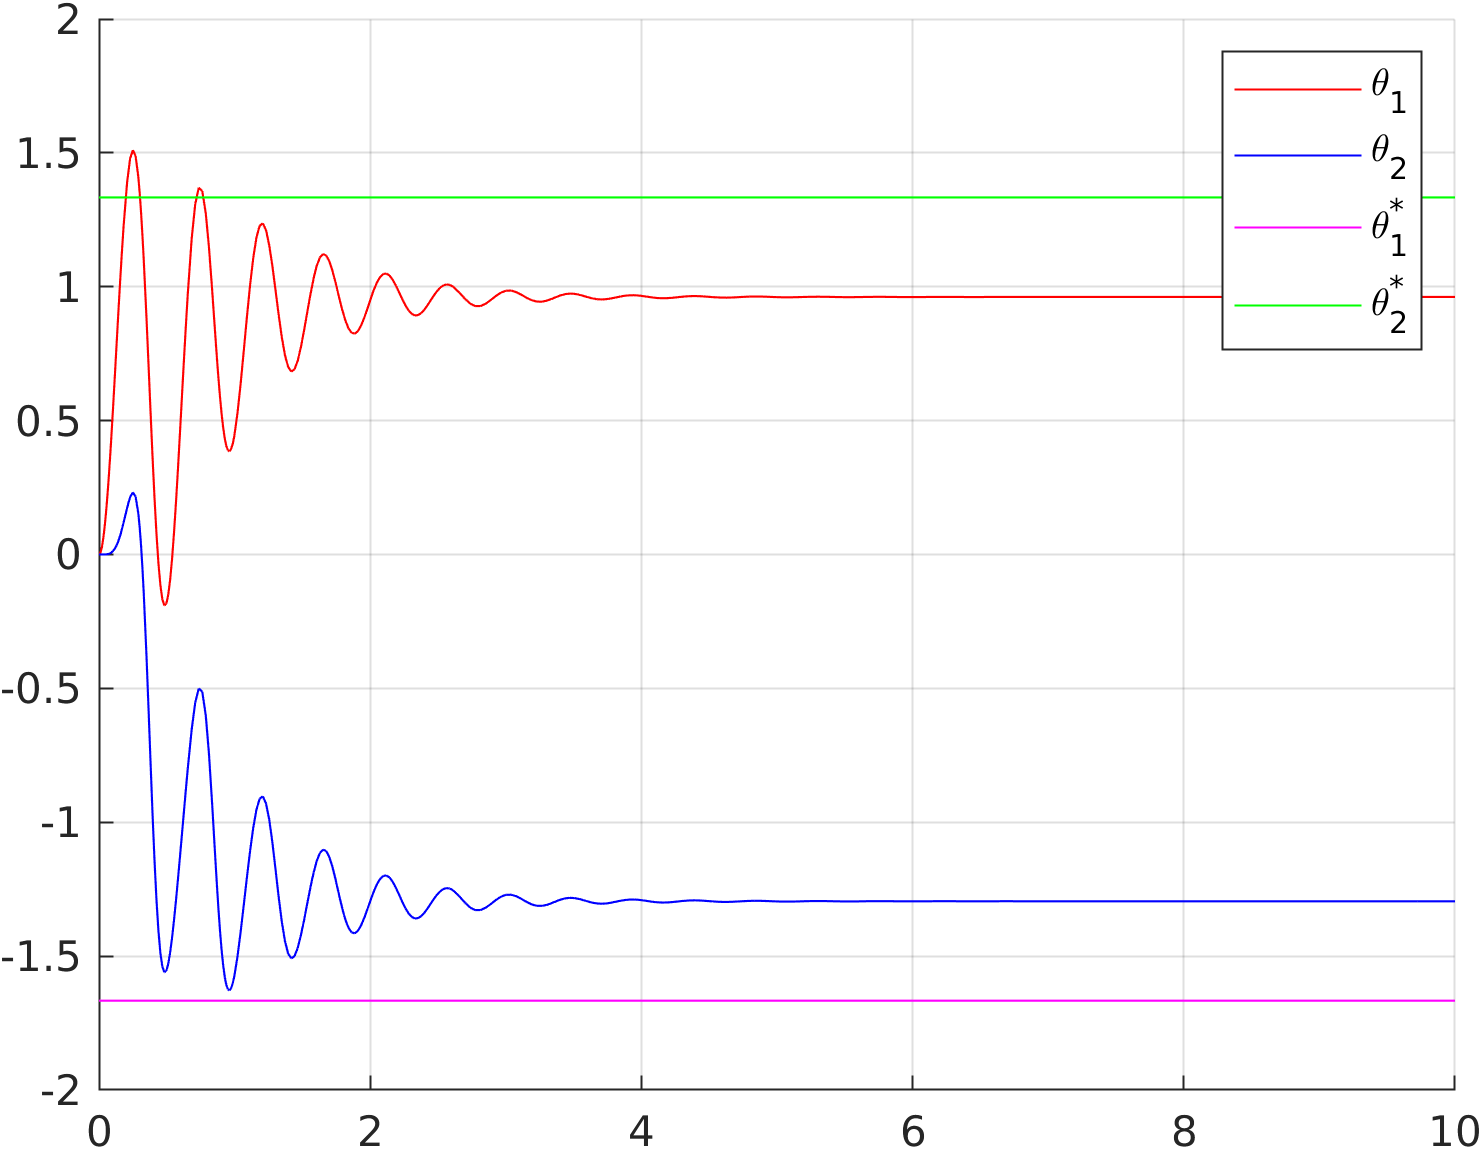
\includegraphics[width=1\textwidth]{Graphics/LinearParameters1.png}
			\end{subfigure}
			\begin{subfigure}{.45\textwidth}
				\centering
				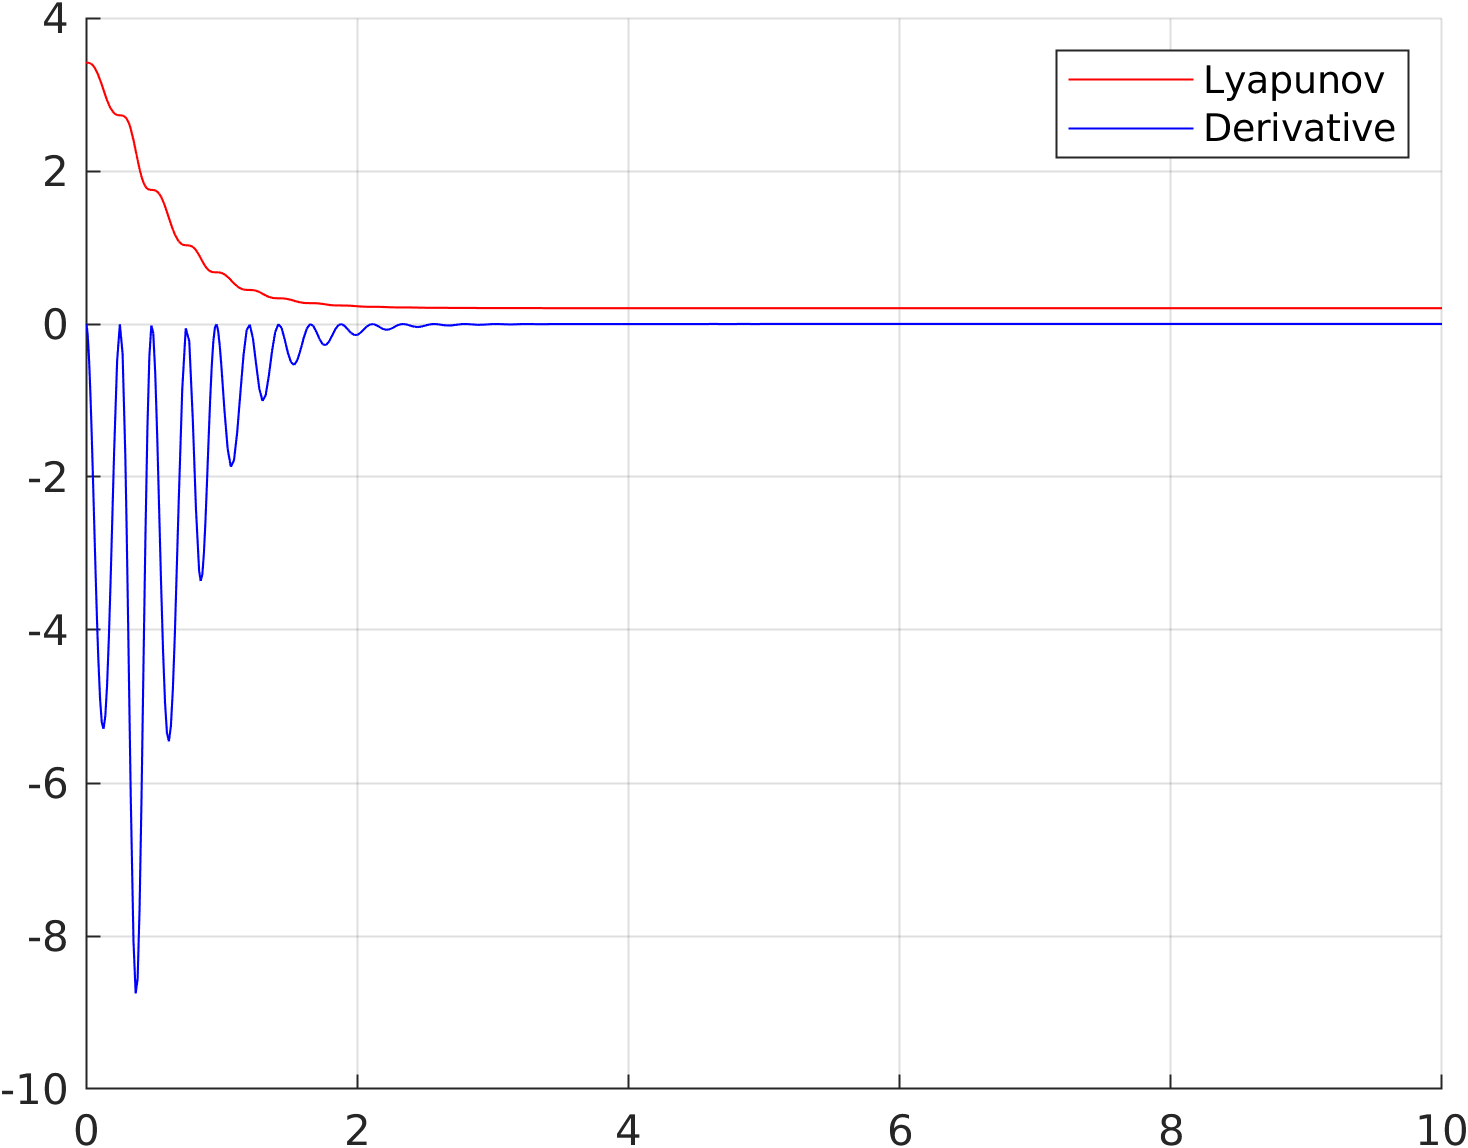
\includegraphics[width=1\textwidth]{Graphics/LinearLyapunov1.png}
			\end{subfigure}%
			\begin{subfigure}{.45\textwidth}
				\centering
				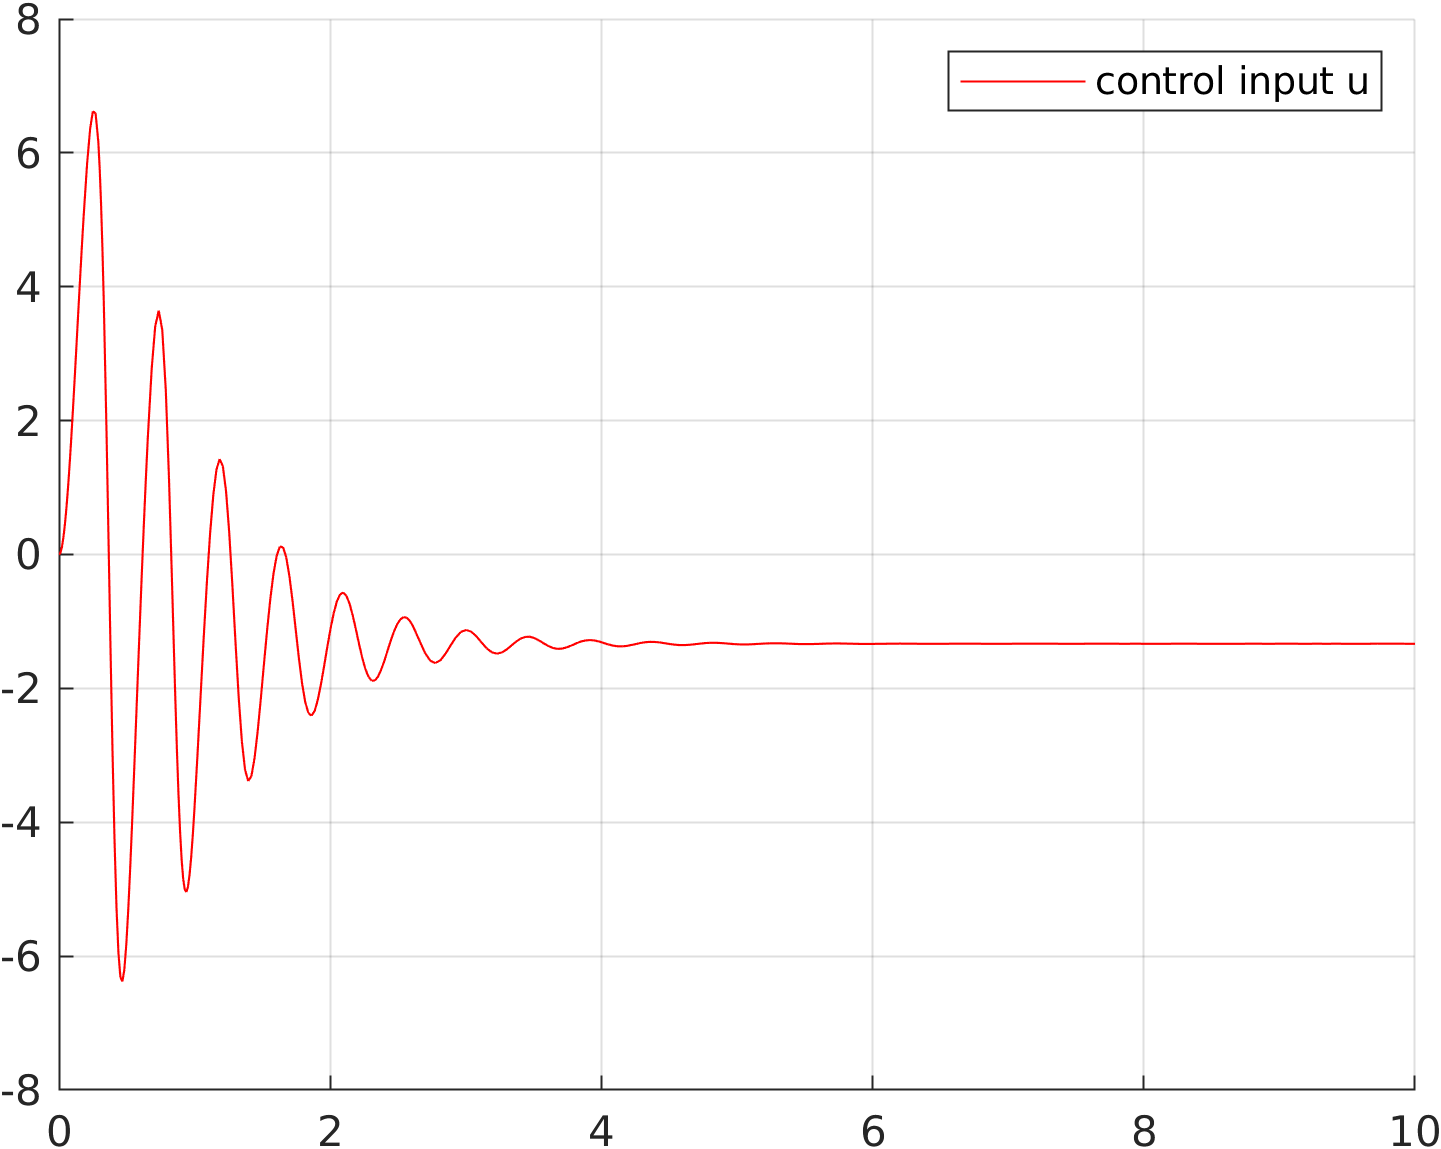
\includegraphics[width=1\textwidth]{Graphics/LinearControl1.png}
			\end{subfigure}
		    \caption{$r(t) = 4$}
		\end{figure}
			
		\begin{figure}[H]
			\centering
			\begin{subfigure}{.45\textwidth}
				\centering
				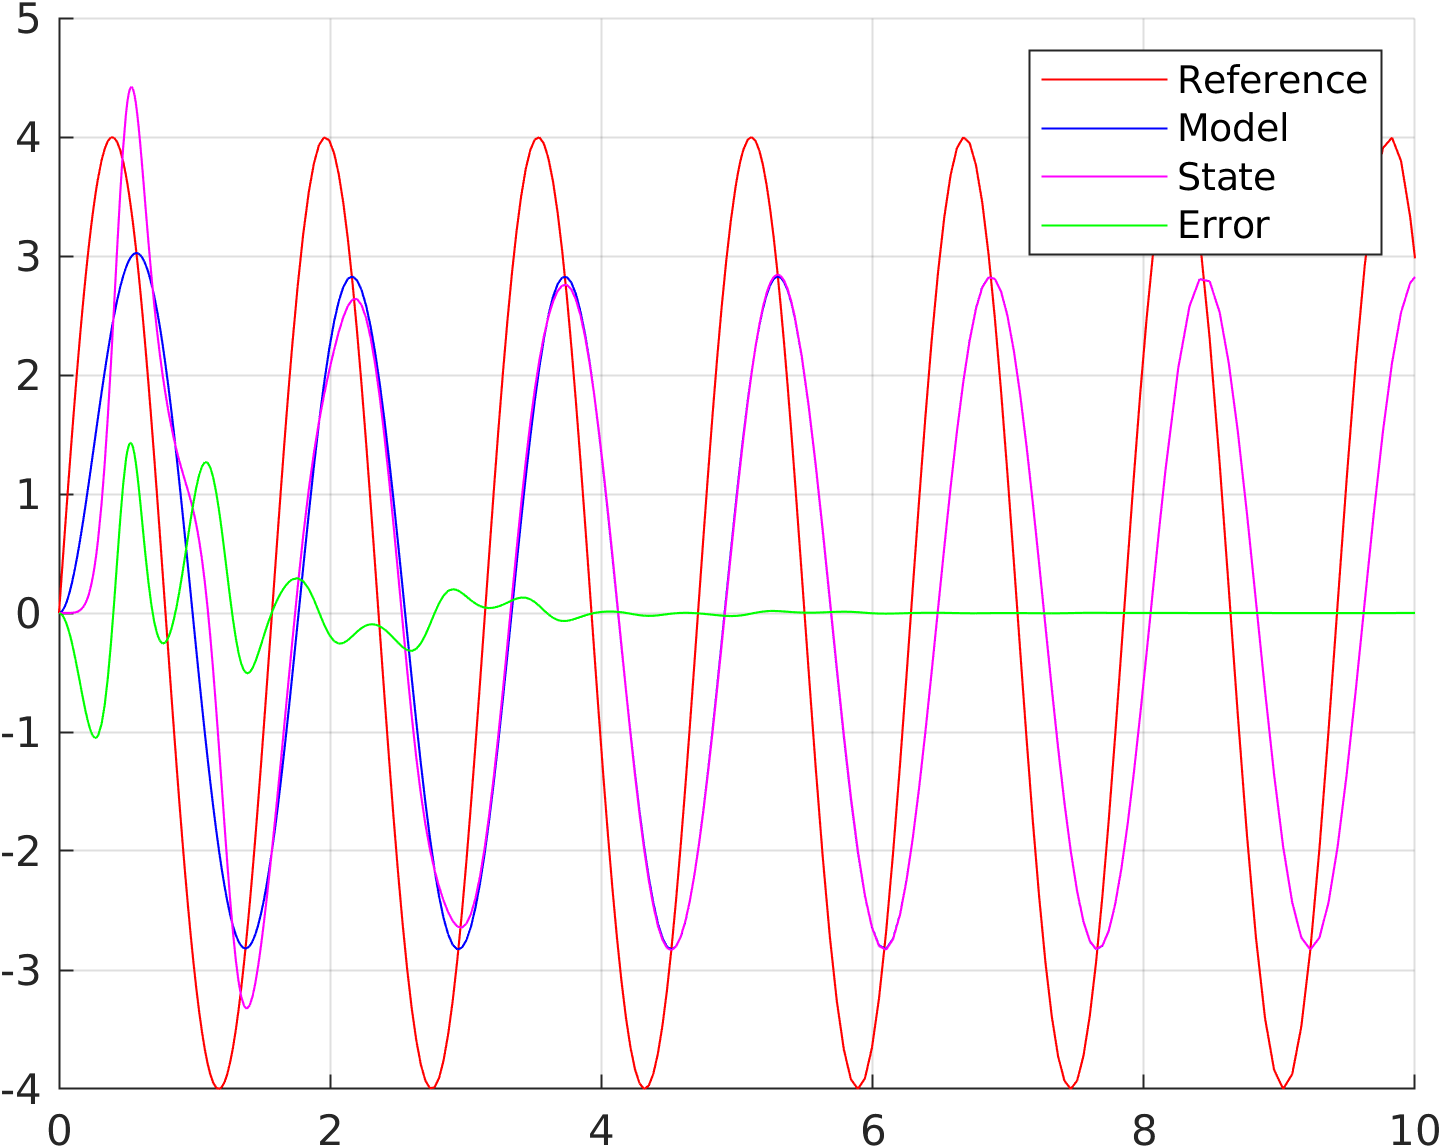
\includegraphics[width=1\textwidth]{Graphics/LinearState2.png}
			\end{subfigure}%
			\begin{subfigure}{.45\textwidth}
				\centering
				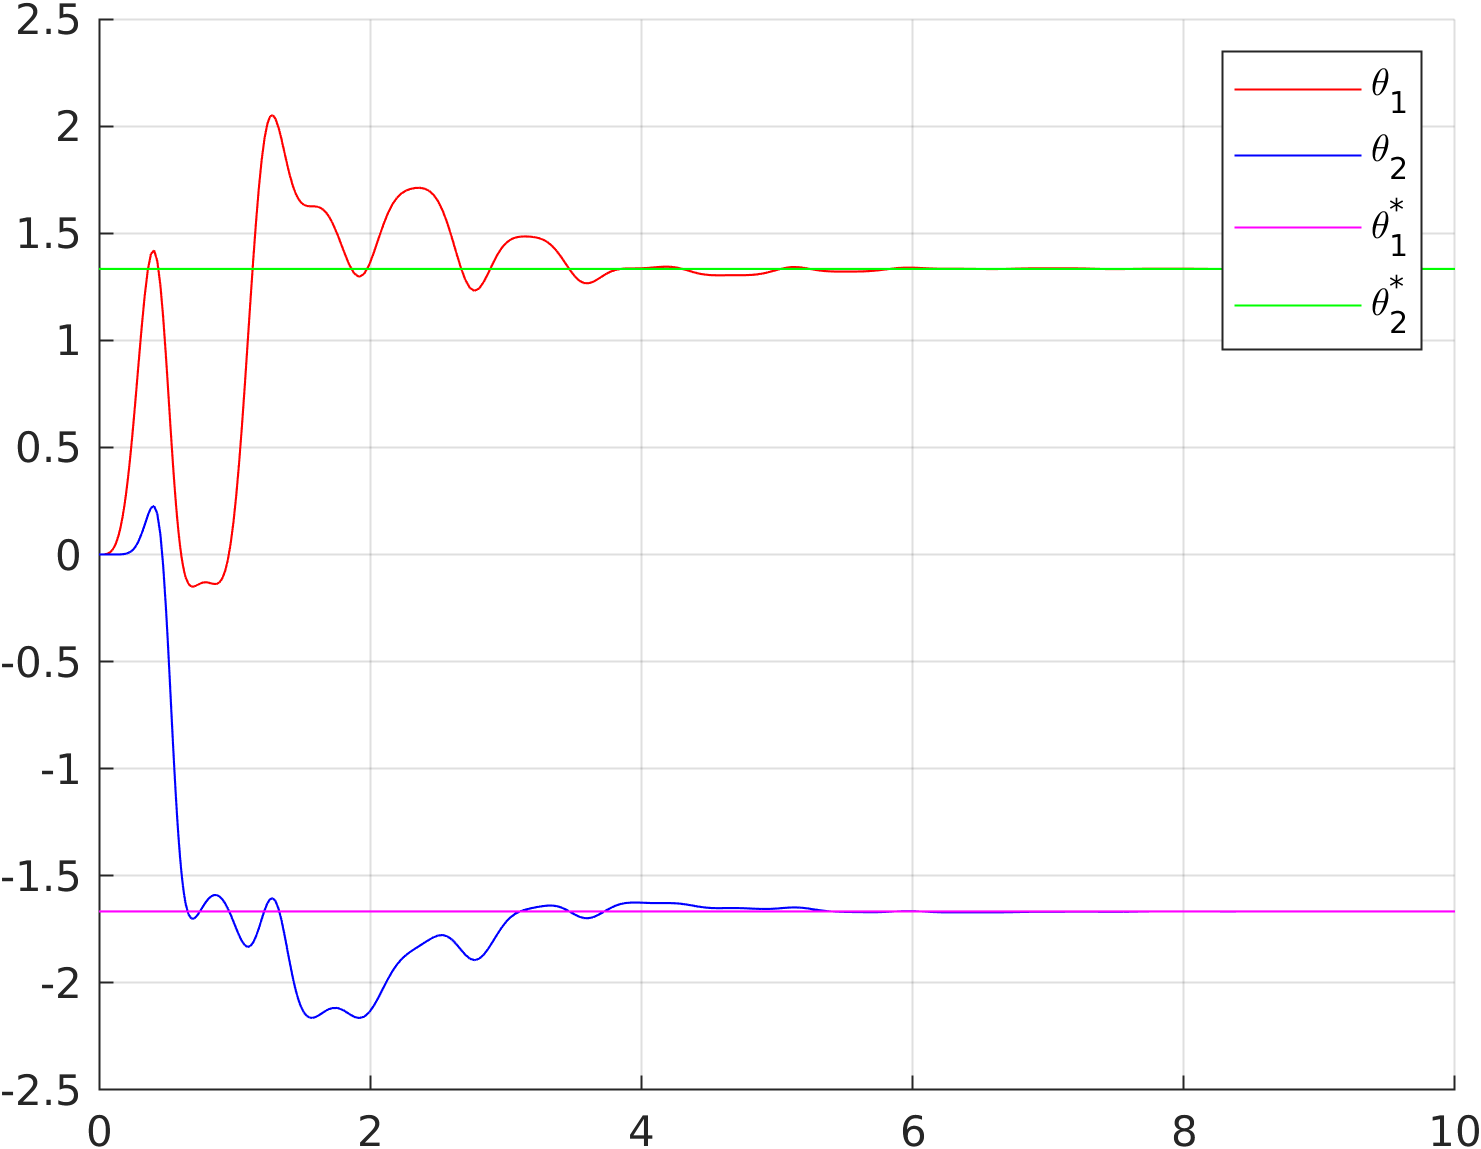
\includegraphics[width=1\textwidth]{Graphics/LinearParameters2.png}
			\end{subfigure}
			\begin{subfigure}{.45\textwidth}
				\centering
				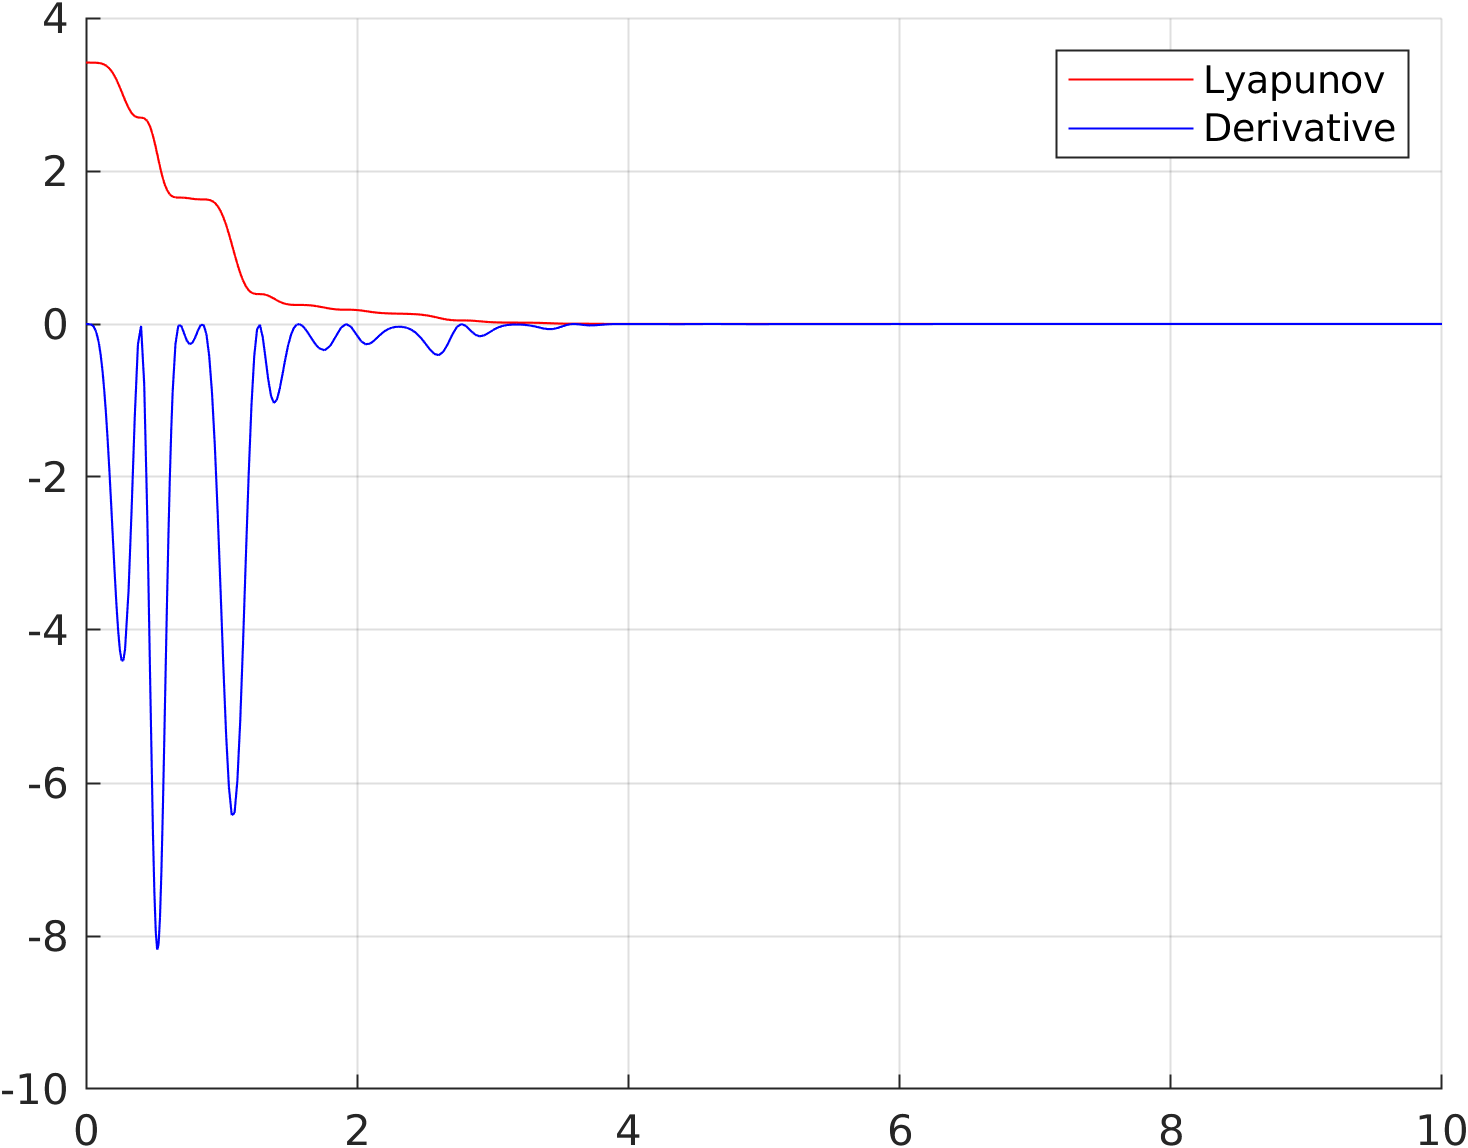
\includegraphics[width=1\textwidth]{Graphics/LinearLyapunov2.png}
			\end{subfigure}%
			\begin{subfigure}{.45\textwidth}
				\centering
				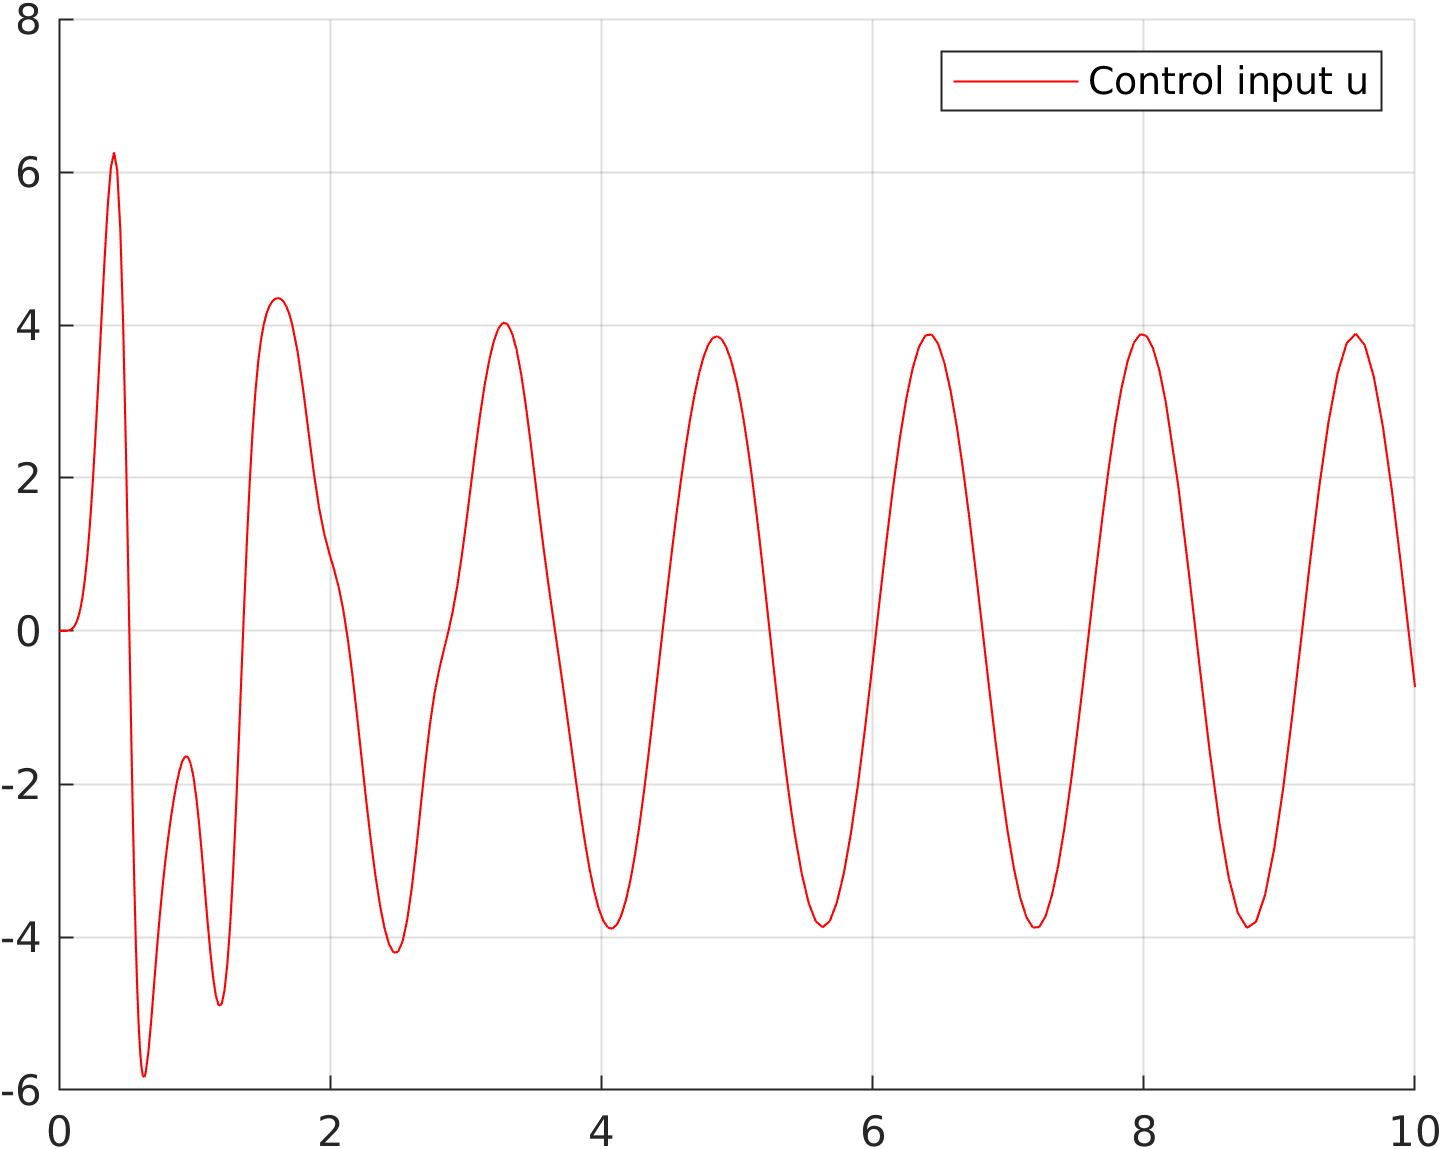
\includegraphics[width=1\textwidth]{Graphics/LinearControl2.png}
			\end{subfigure}
		    \caption{$r(t) = 4\sin(4t)$}
		\end{figure}
	
		\begin{figure}[H]
			\centering
			\begin{subfigure}{.45\textwidth}
				\centering
				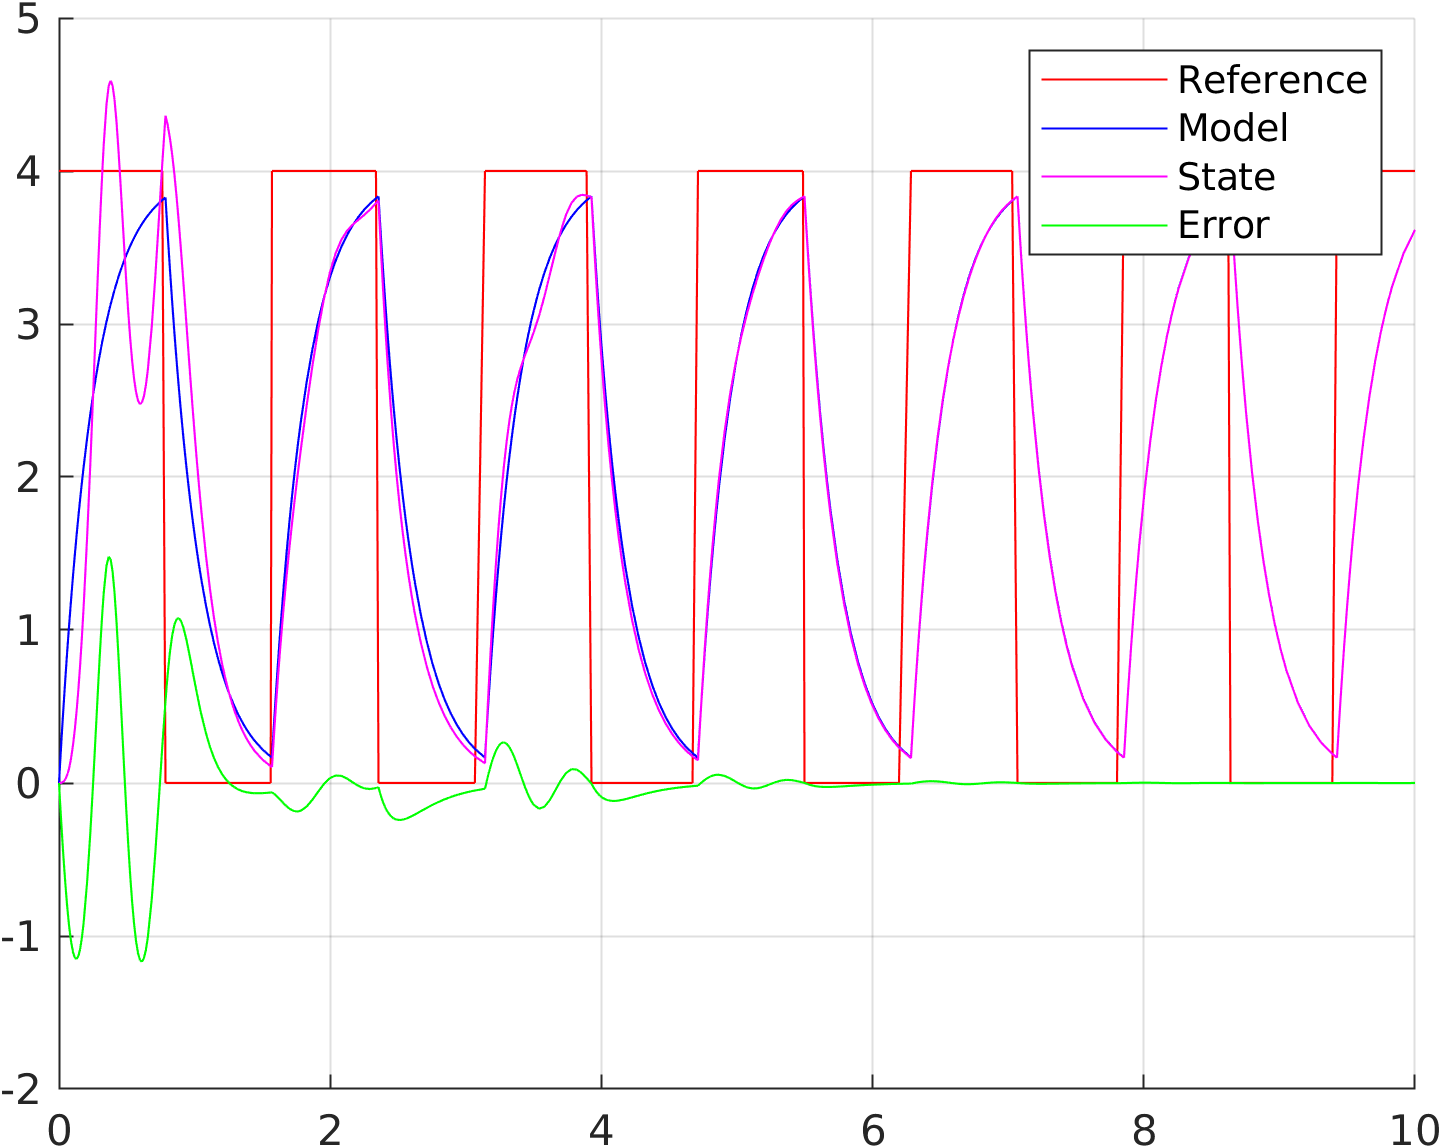
\includegraphics[width=1\textwidth]{Graphics/LinearState3.png}
			\end{subfigure}%
			\begin{subfigure}{.45\textwidth}
				\centering
				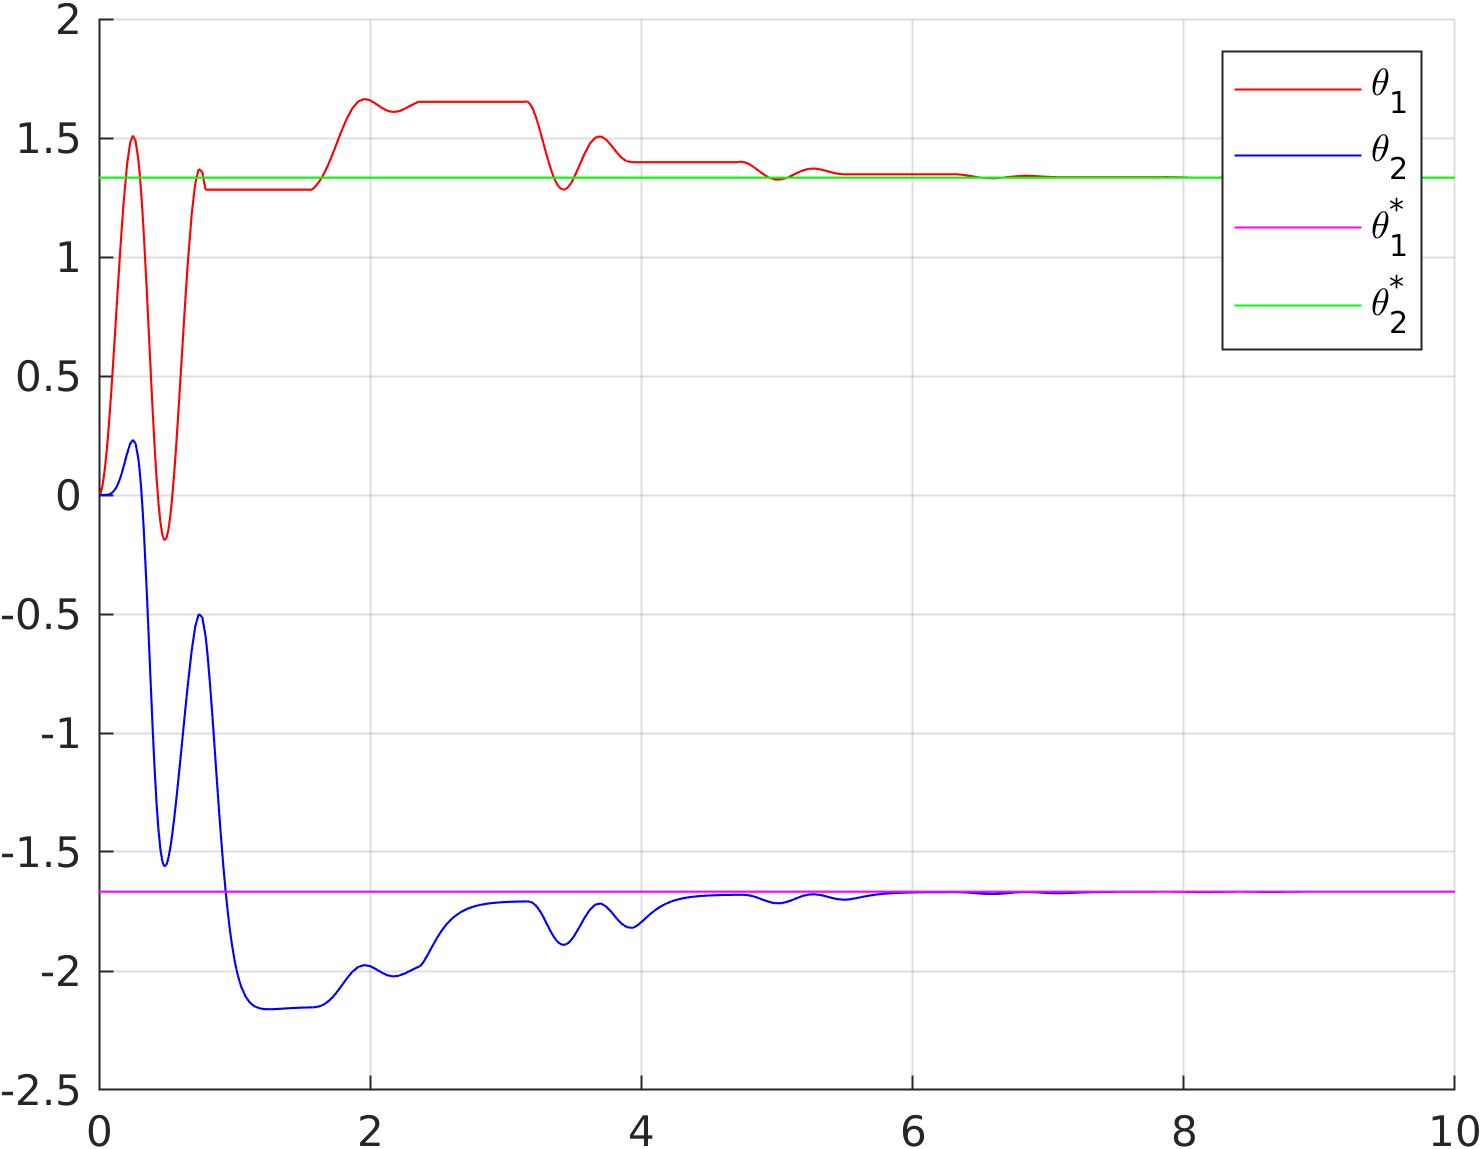
\includegraphics[width=1\textwidth]{Graphics/LinearParameters3.png}
			\end{subfigure}
			\begin{subfigure}{.45\textwidth}
				\centering
				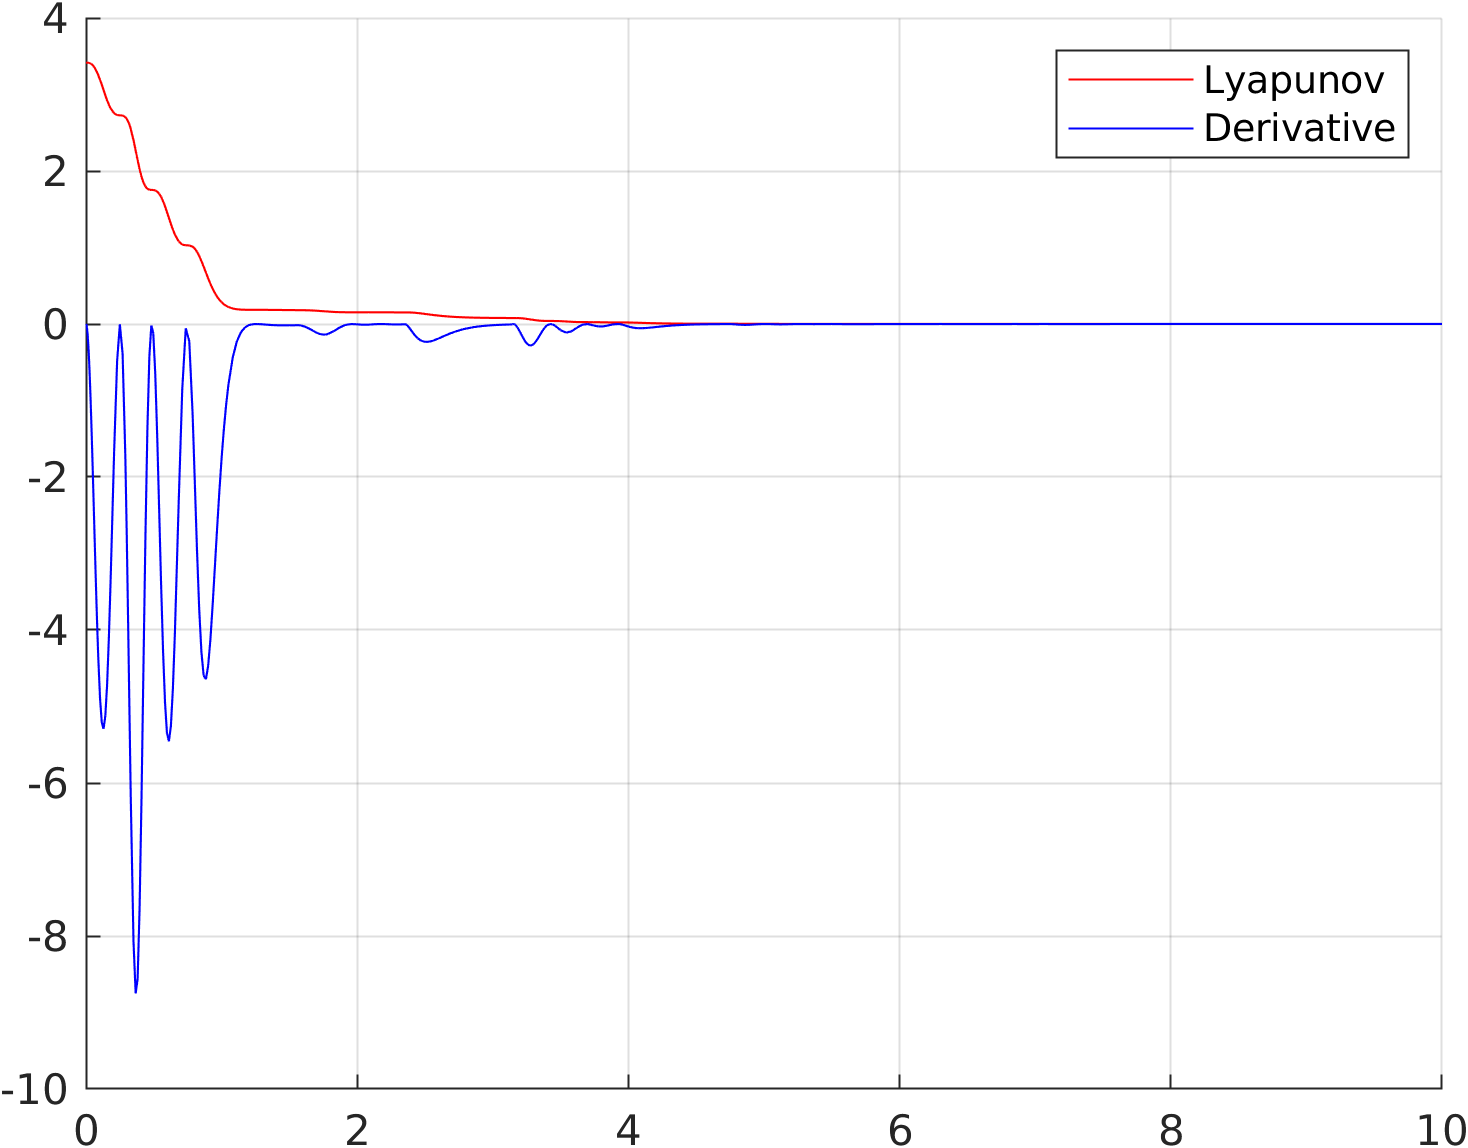
\includegraphics[width=1\textwidth]{Graphics/LinearLyapunov3.png}
			\end{subfigure}%
			\begin{subfigure}{.45\textwidth}
				\centering
				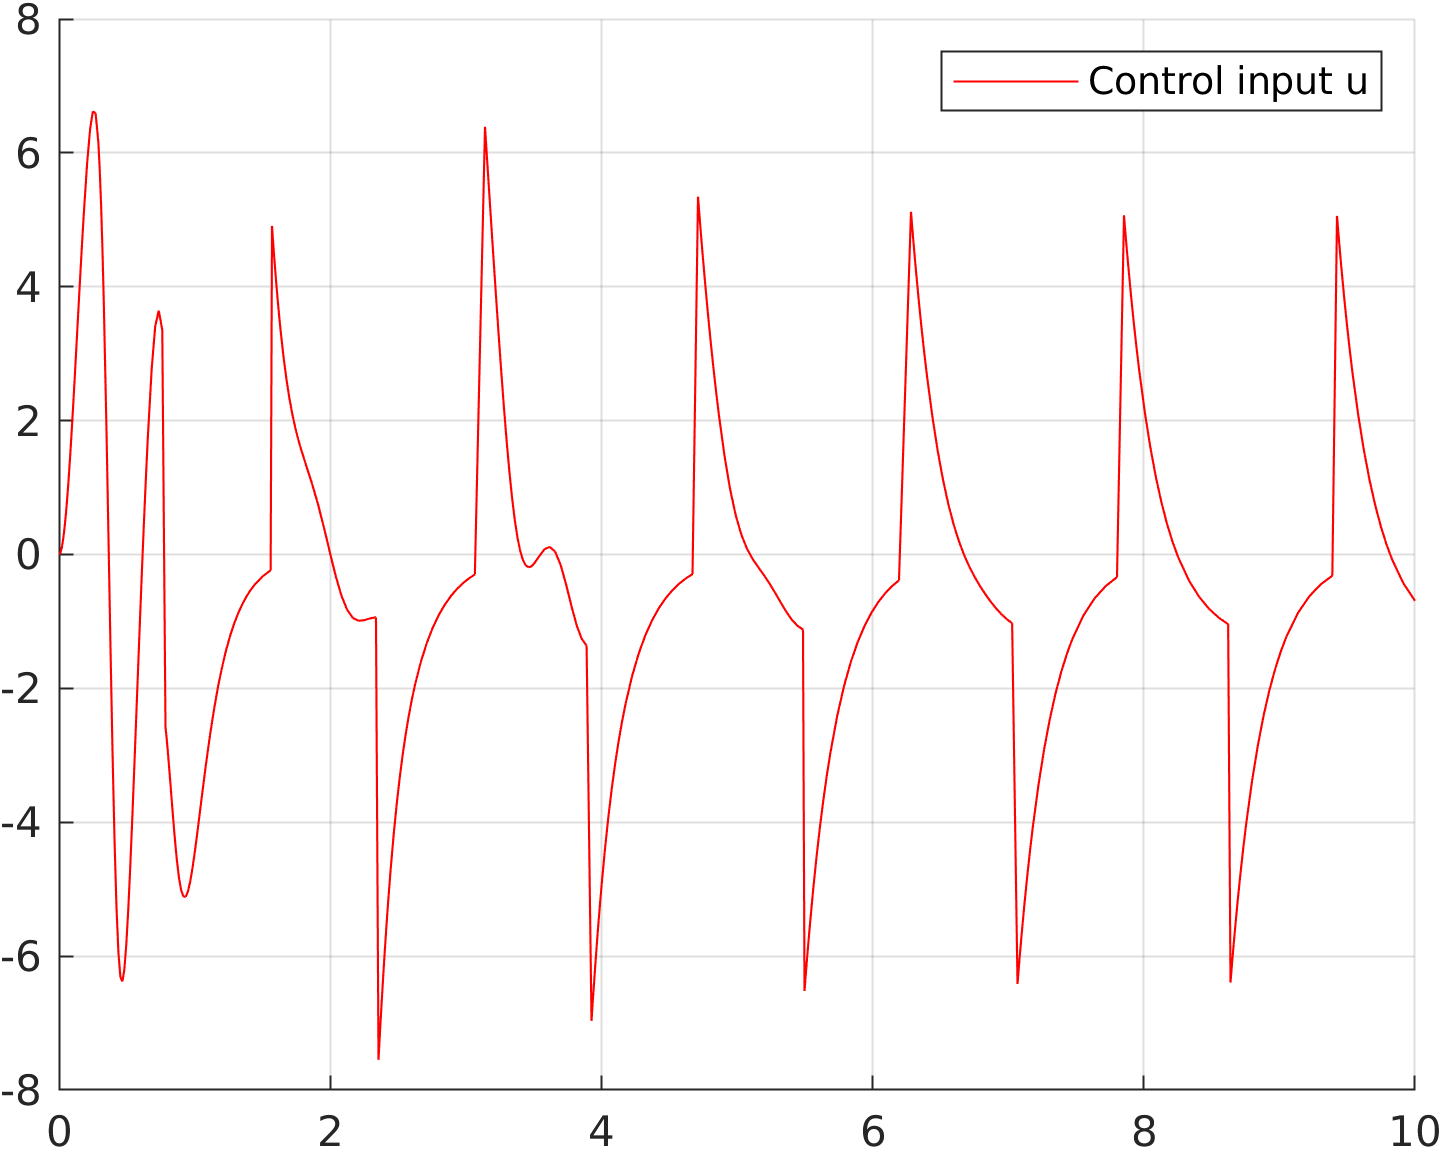
\includegraphics[width=1\textwidth]{Graphics/LinearControl3.png}
			\end{subfigure}
		\caption{$r(t) = 4\operatorname{rect}(\frac{2}{\pi}t)$, where $\operatorname{rect}(\frac{2}{\pi}t)$ has period $\pi/2$}
		\label{fig:rect1}
		\end{figure}
	
		\begin{figure}[H]
			\centering
			\begin{subfigure}{.45\textwidth}
				\centering
				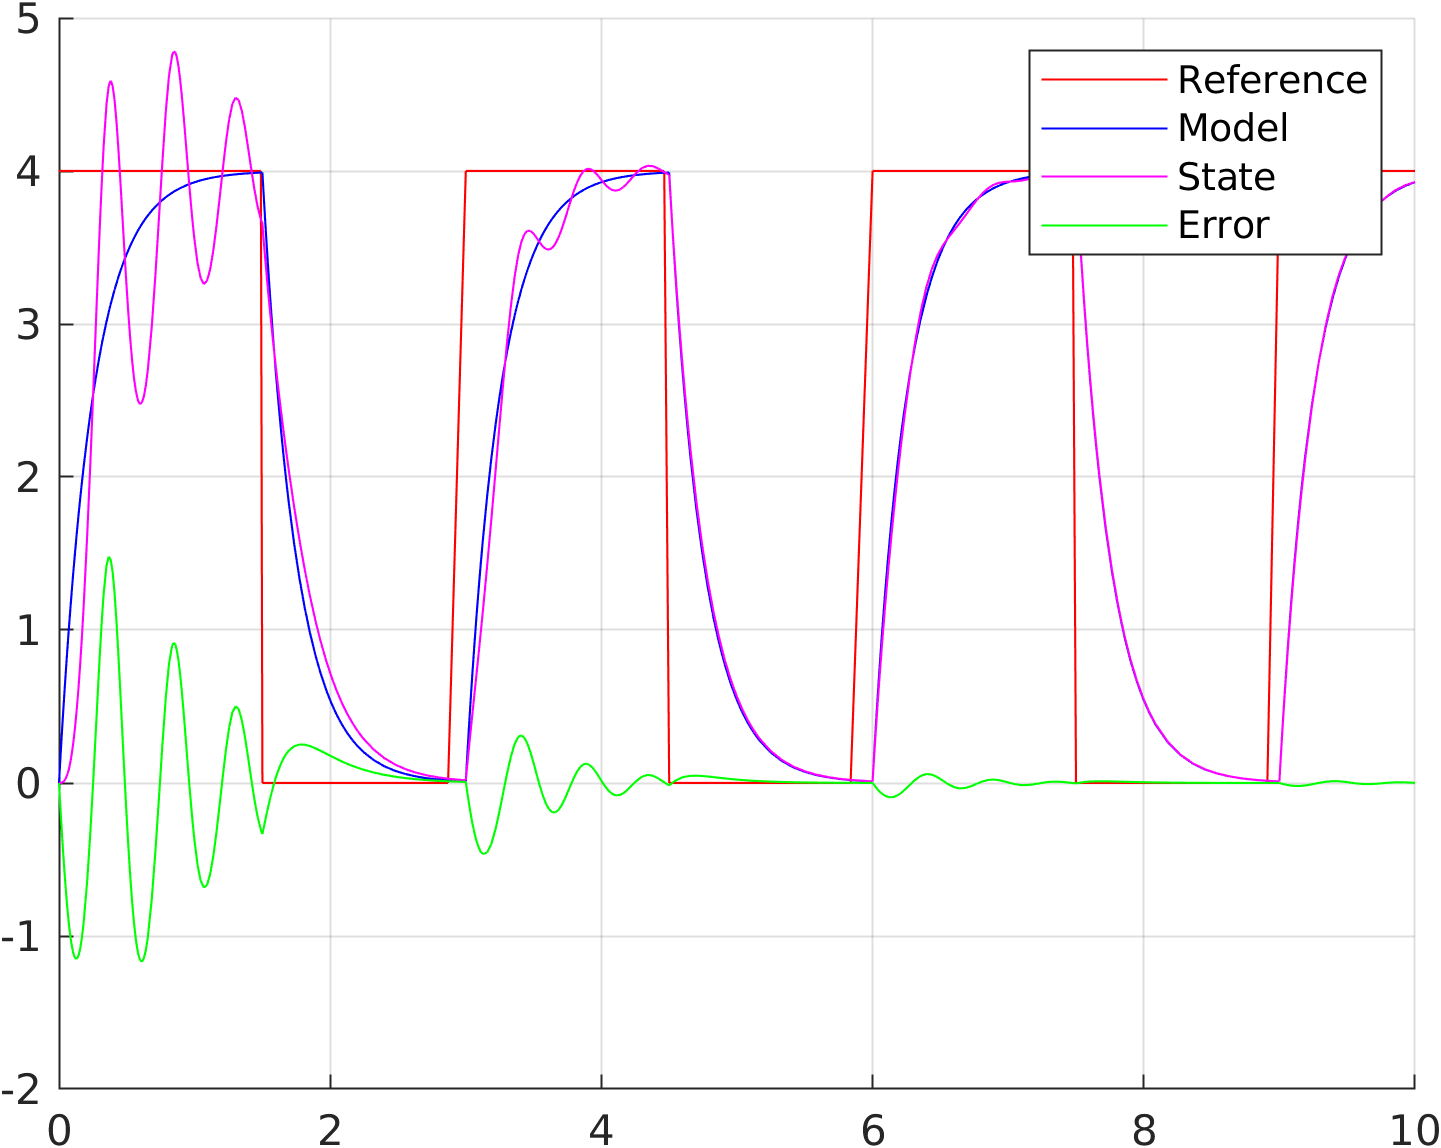
\includegraphics[width=1\textwidth]{Graphics/LinearState4.png}
			\end{subfigure}%
			\begin{subfigure}{.45\textwidth}
				\centering
				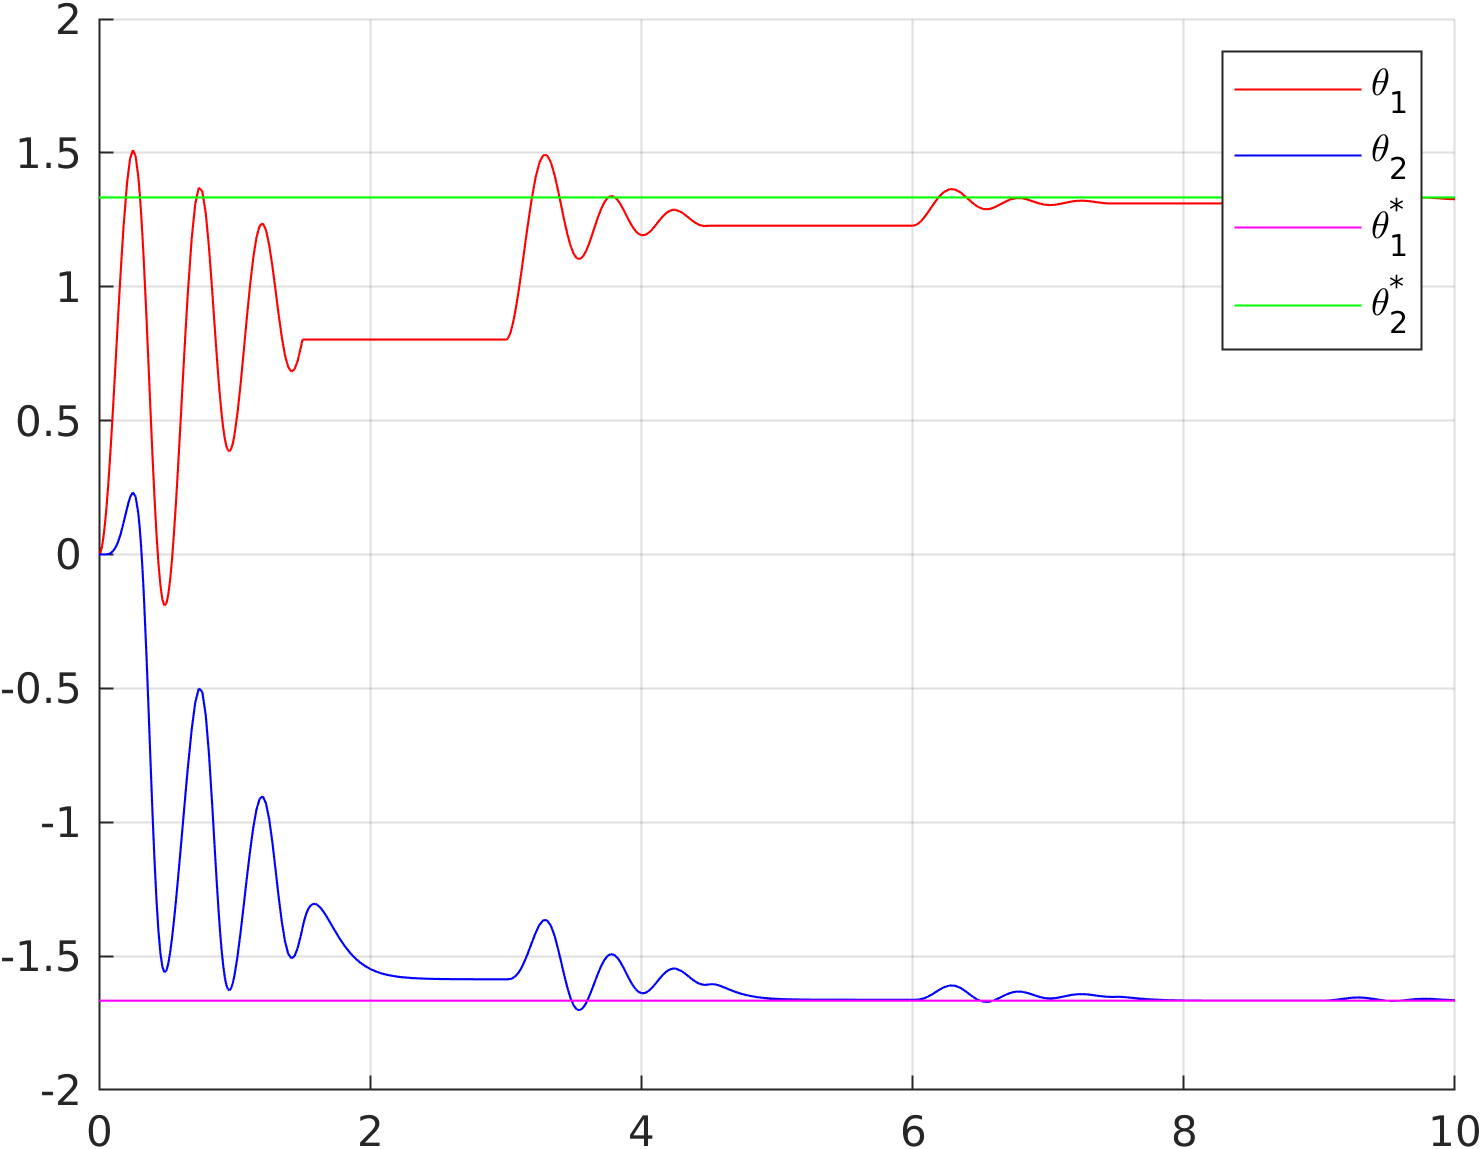
\includegraphics[width=1\textwidth]{Graphics/LinearParameters4.png}
			\end{subfigure}
			\begin{subfigure}{.45\textwidth}
				\centering
				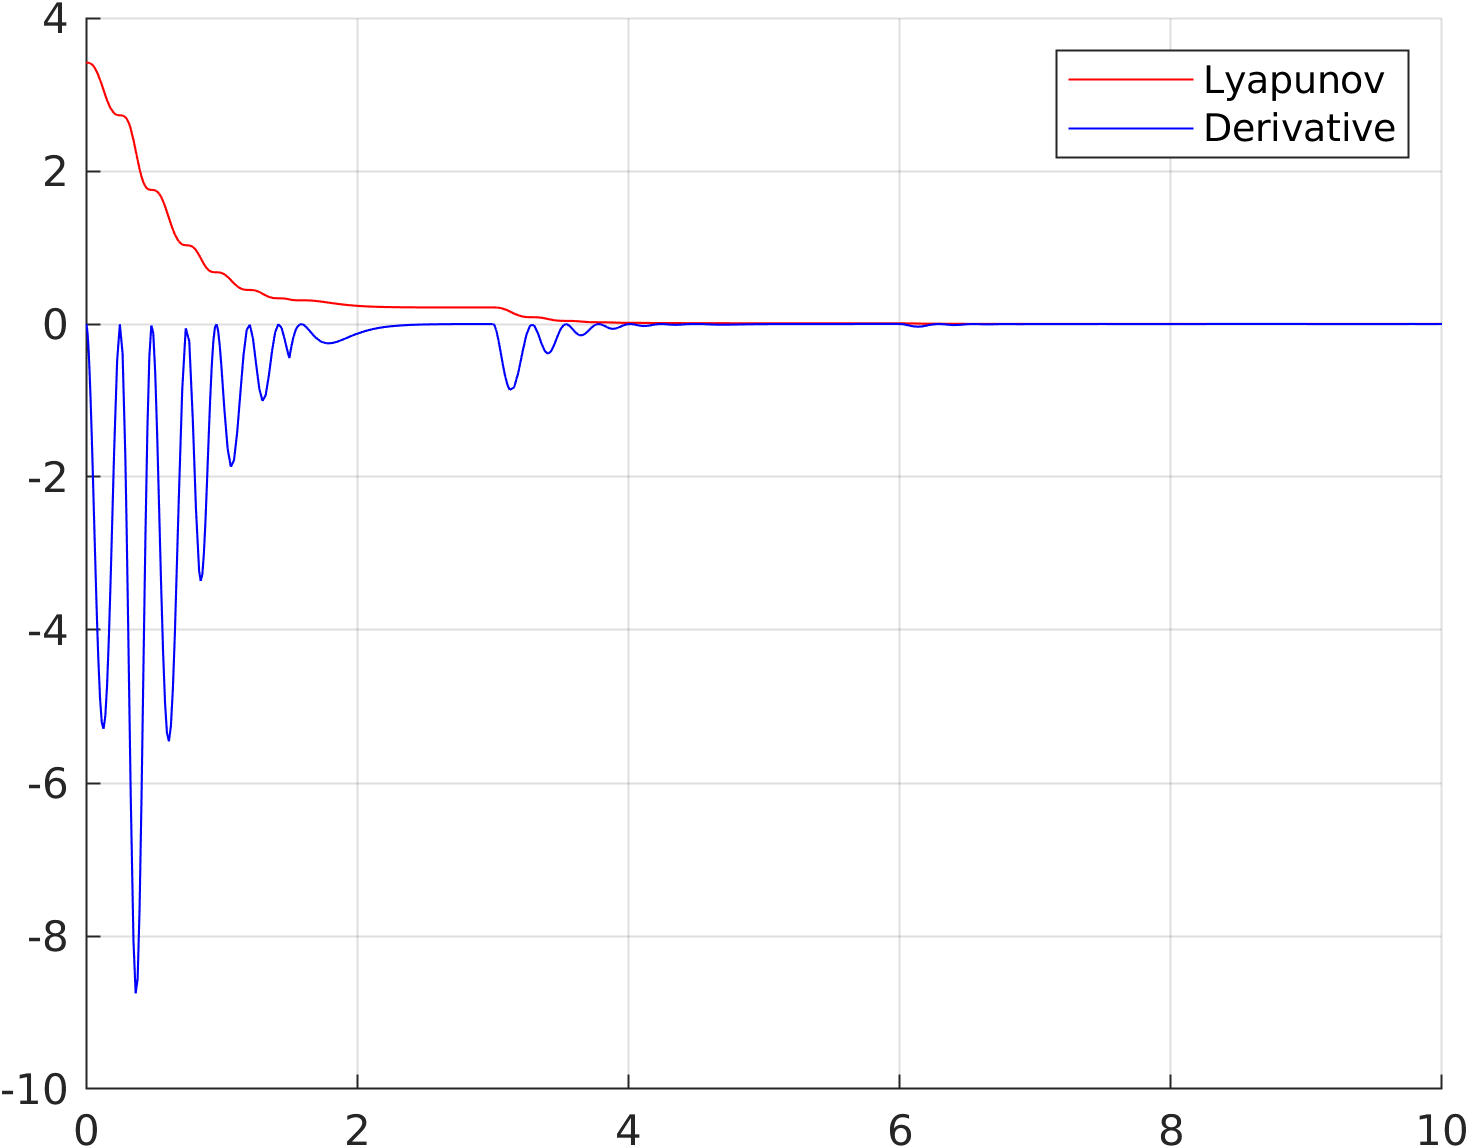
\includegraphics[width=1\textwidth]{Graphics/LinearLyapunov4.png}
			\end{subfigure}%
			\begin{subfigure}{.45\textwidth}
				\centering
				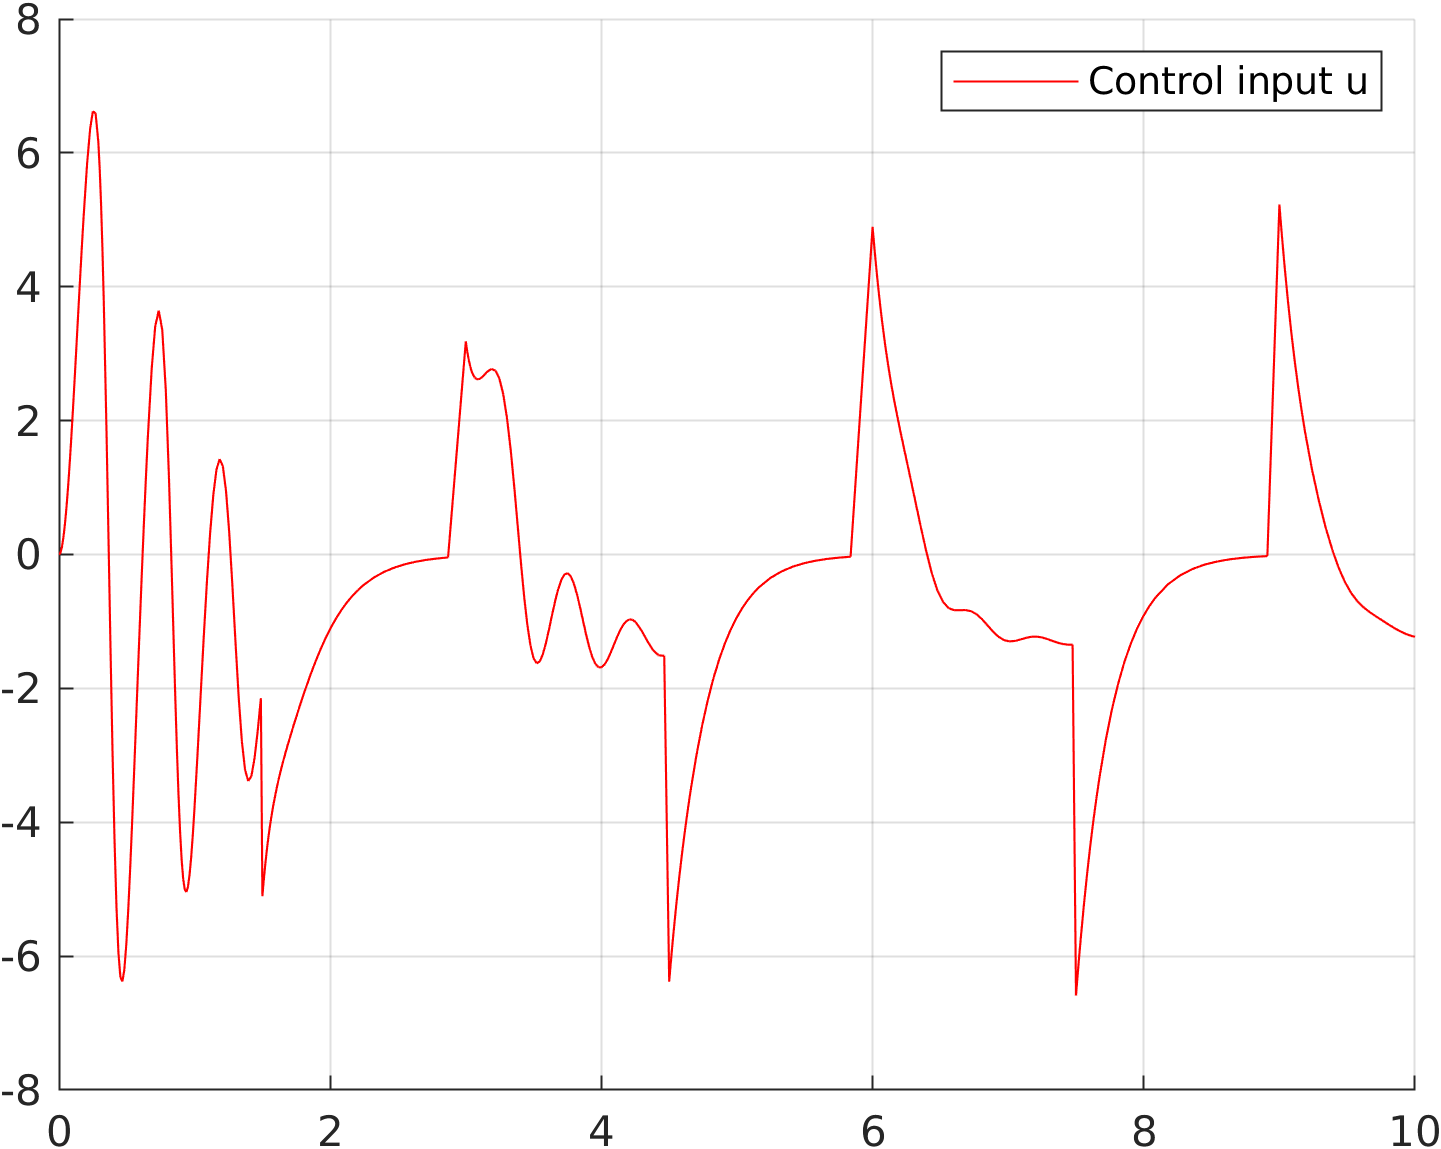
\includegraphics[width=1\textwidth]{Graphics/LinearControl4.png}
			\end{subfigure}
		\caption{$r(t) = 4\operatorname{rect}(t/3)$, where $\operatorname{rect}(t/3)$ has period $3$}
		\label{fig:rect2}
		\end{figure}
	 
		\begin{figure}[H]
			\centering
			\begin{subfigure}{.45\textwidth}
				\centering
				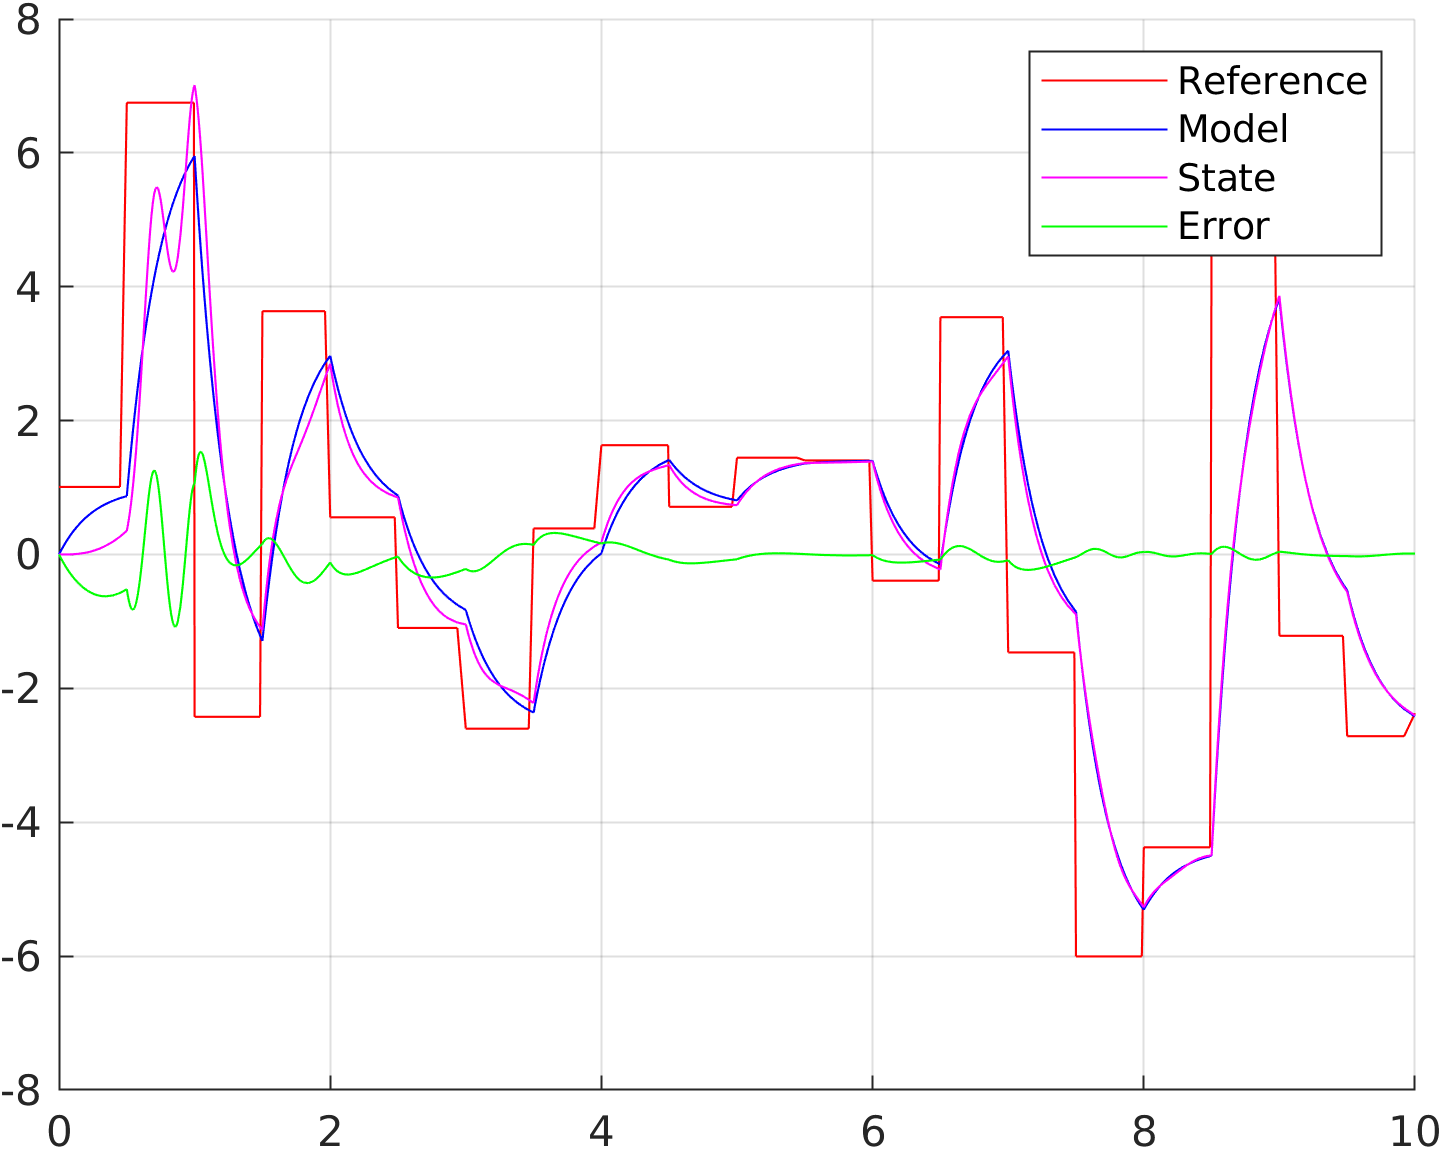
\includegraphics[width=1\textwidth]{Graphics/LinearState5.png}
			\end{subfigure}%
			\begin{subfigure}{.45\textwidth}
				\centering
				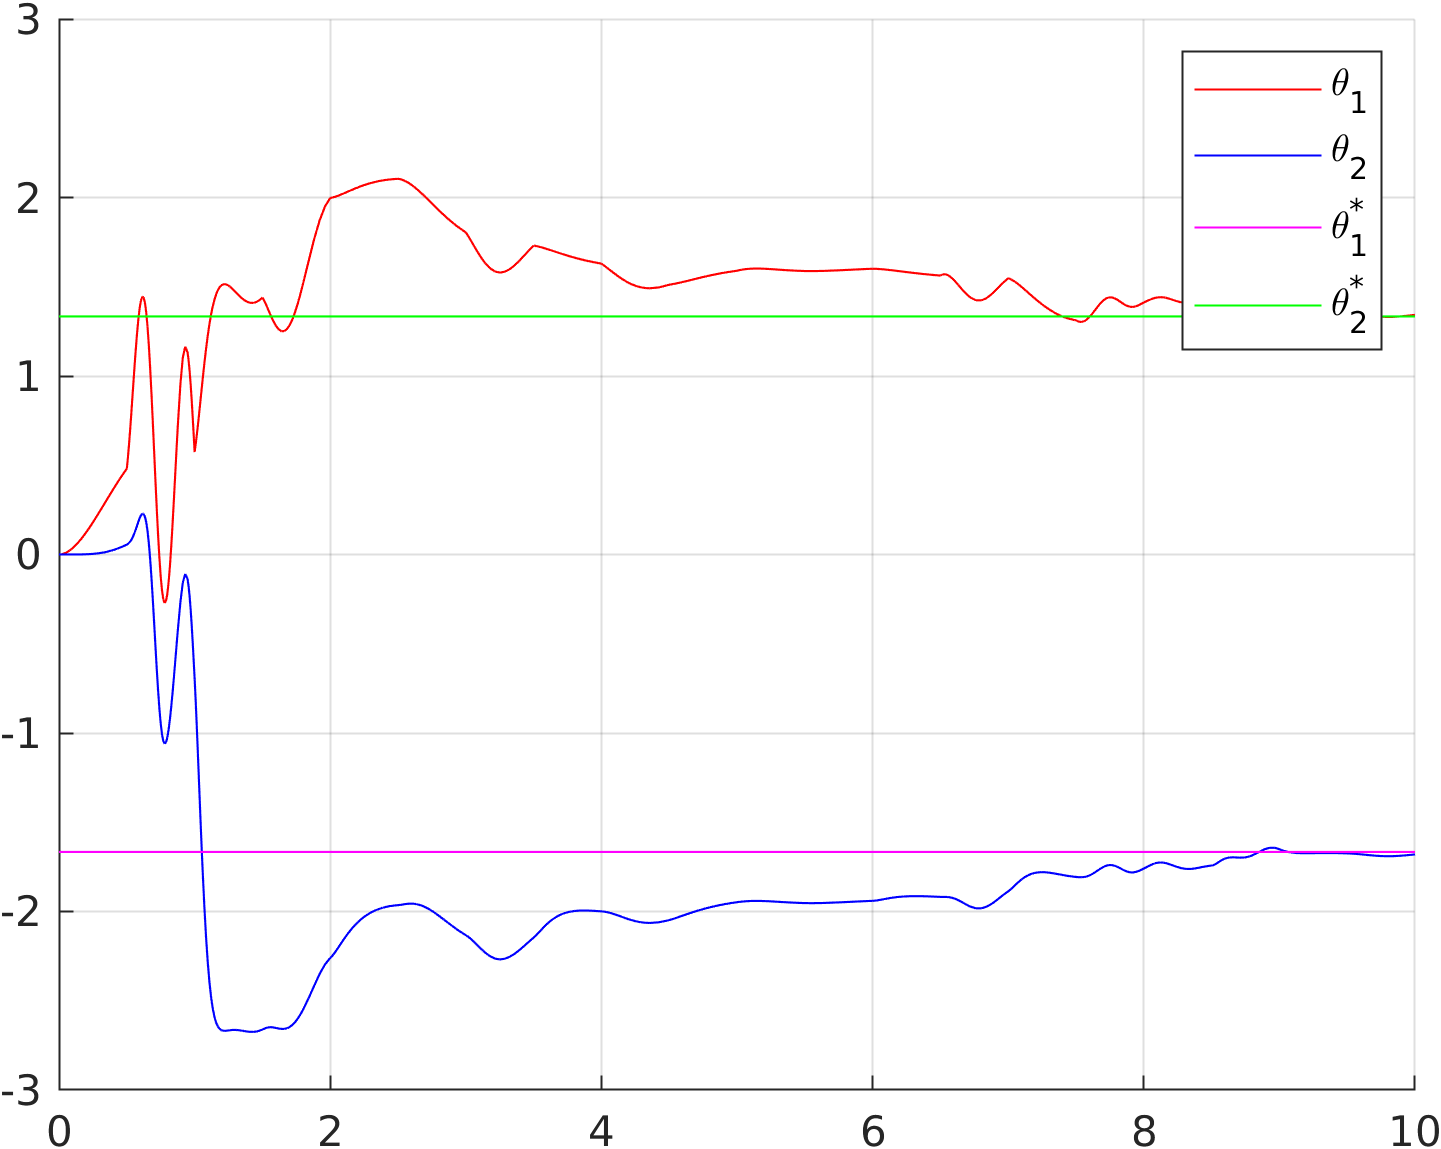
\includegraphics[width=1\textwidth]{Graphics/LinearParameters5.png}
			\end{subfigure}
			\begin{subfigure}{.45\textwidth}
				\centering
				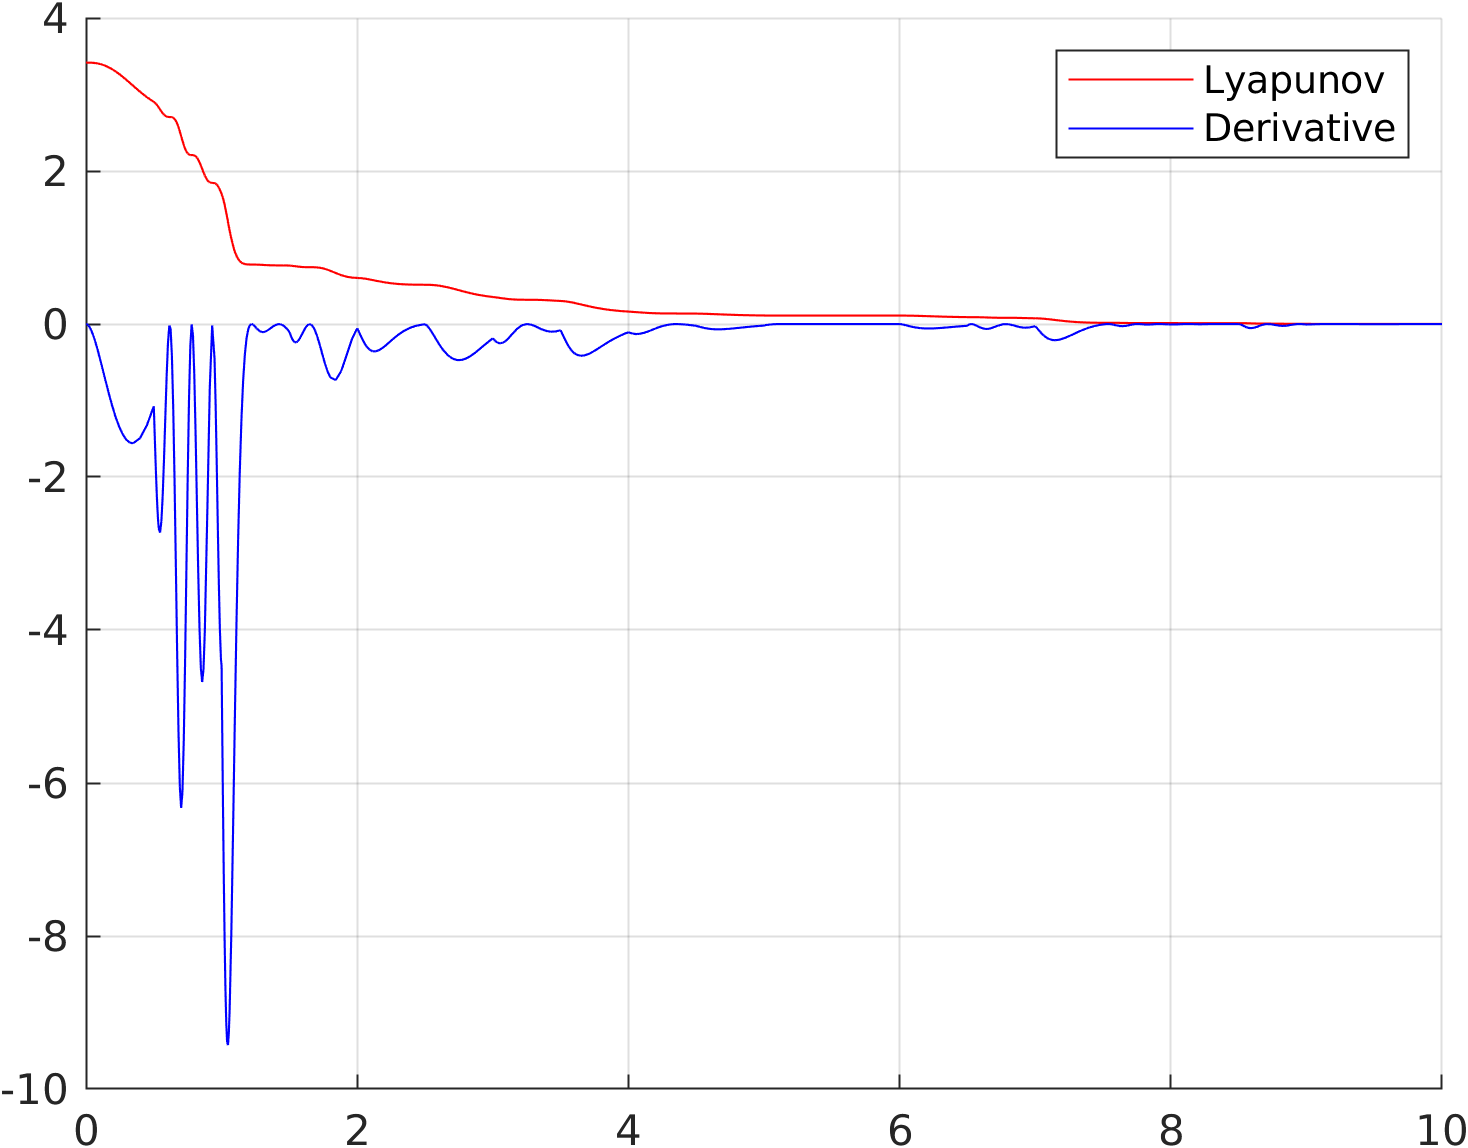
\includegraphics[width=1\textwidth]{Graphics/LinearLyapunov5.png}
			\end{subfigure}%
			\begin{subfigure}{.45\textwidth}
				\centering
				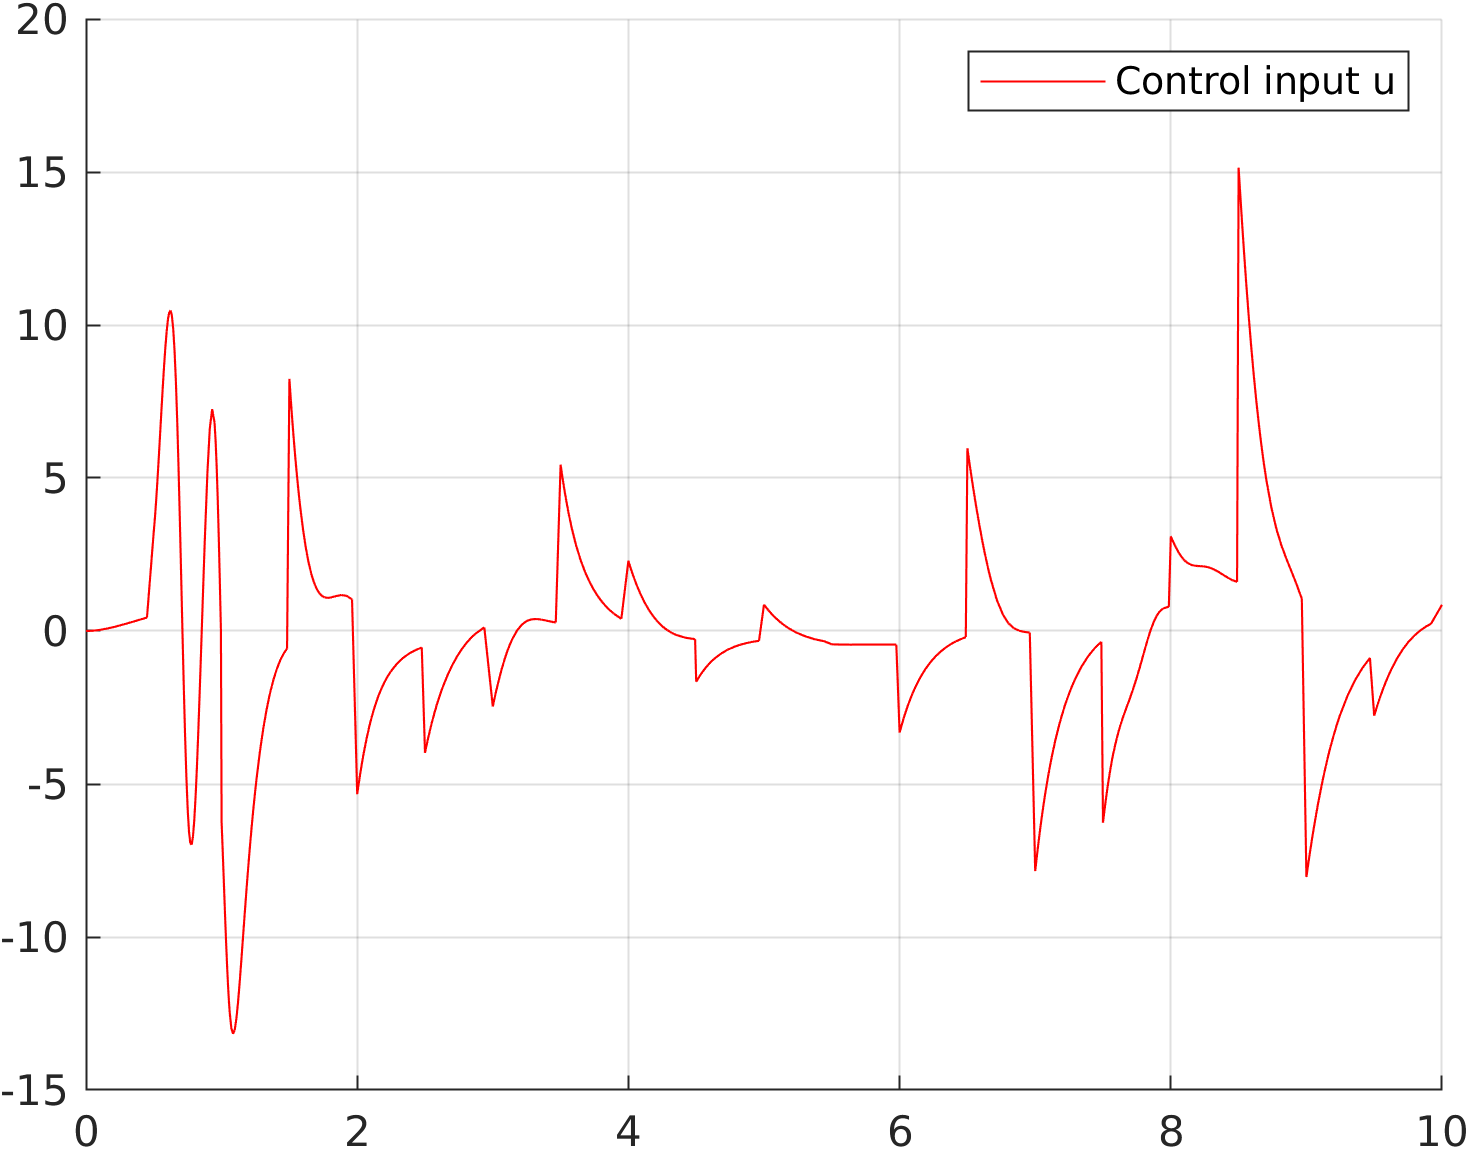
\includegraphics[width=1\textwidth]{Graphics/LinearControl5.png}
			\end{subfigure}
		\caption{$r(t)$ - band limited Gaussian white noise of power $4$ and sample time $0.5$}
		\label{fig:gaussian}
		\end{figure}
	
	\begin{center}
		\begin{tabular}{c|c}
			Signal & Values at $T = 10s$ \\ \hline
			$r(t) = 4$ & $\theta_a = -1.30$, $k = 0.96$\\
			$r(t) = 4\sin(4t)$ & $\theta_a = -1.67$, $k = 1.33$\\
			$r(t) = 4\operatorname{rect}(\frac{2}{\pi}t)$ & $\theta_a = -1.67$, $k = 1.33$\\
			$r(t) = 4\operatorname{rect}(t/3)$ & $\theta_a = -1.67$, $k = 1.33$\\
			 band limited Gaussian white noise & $\theta_a = -1.68$, $k = 1.34$\\
		\end{tabular}
	\end{center}
	
	For $r(t) = 4$ the parameters did not converge to the true parameters, however for the other signals they (approximately) did. 
	For high-frequency reference signals the parameter convergence was faster than for the low-frequency ones, which can be seen from the learning rate in Figures
	\ref{fig:rect1} and \ref{fig:rect2}. 
	This can be explained by the intuition that signals of higher frequency have more "information" and thus reveal about the given unknown system than low-frequency or even constant signals.
	Ideally they should converge to  the true values if there are no two systems of different parameters that have the same output on the same reference signal, i.e. the system model is uniquely determined by the input-output pair.
	But it appears that the periodicity of the reference signal does also play a role for the convergence rate of the parameters, since if the signal is not periodic as in Figure \ref{fig:gaussian}, then the learning is also slower, despite the "frequency" being high.
	
	\subsection*{Nonlinear plant}
	
	\subsubsection*{All parameters unknown}
	Here is the plot of the nonlinear function $f$:
	\begin{figure}[H]
		\centering
		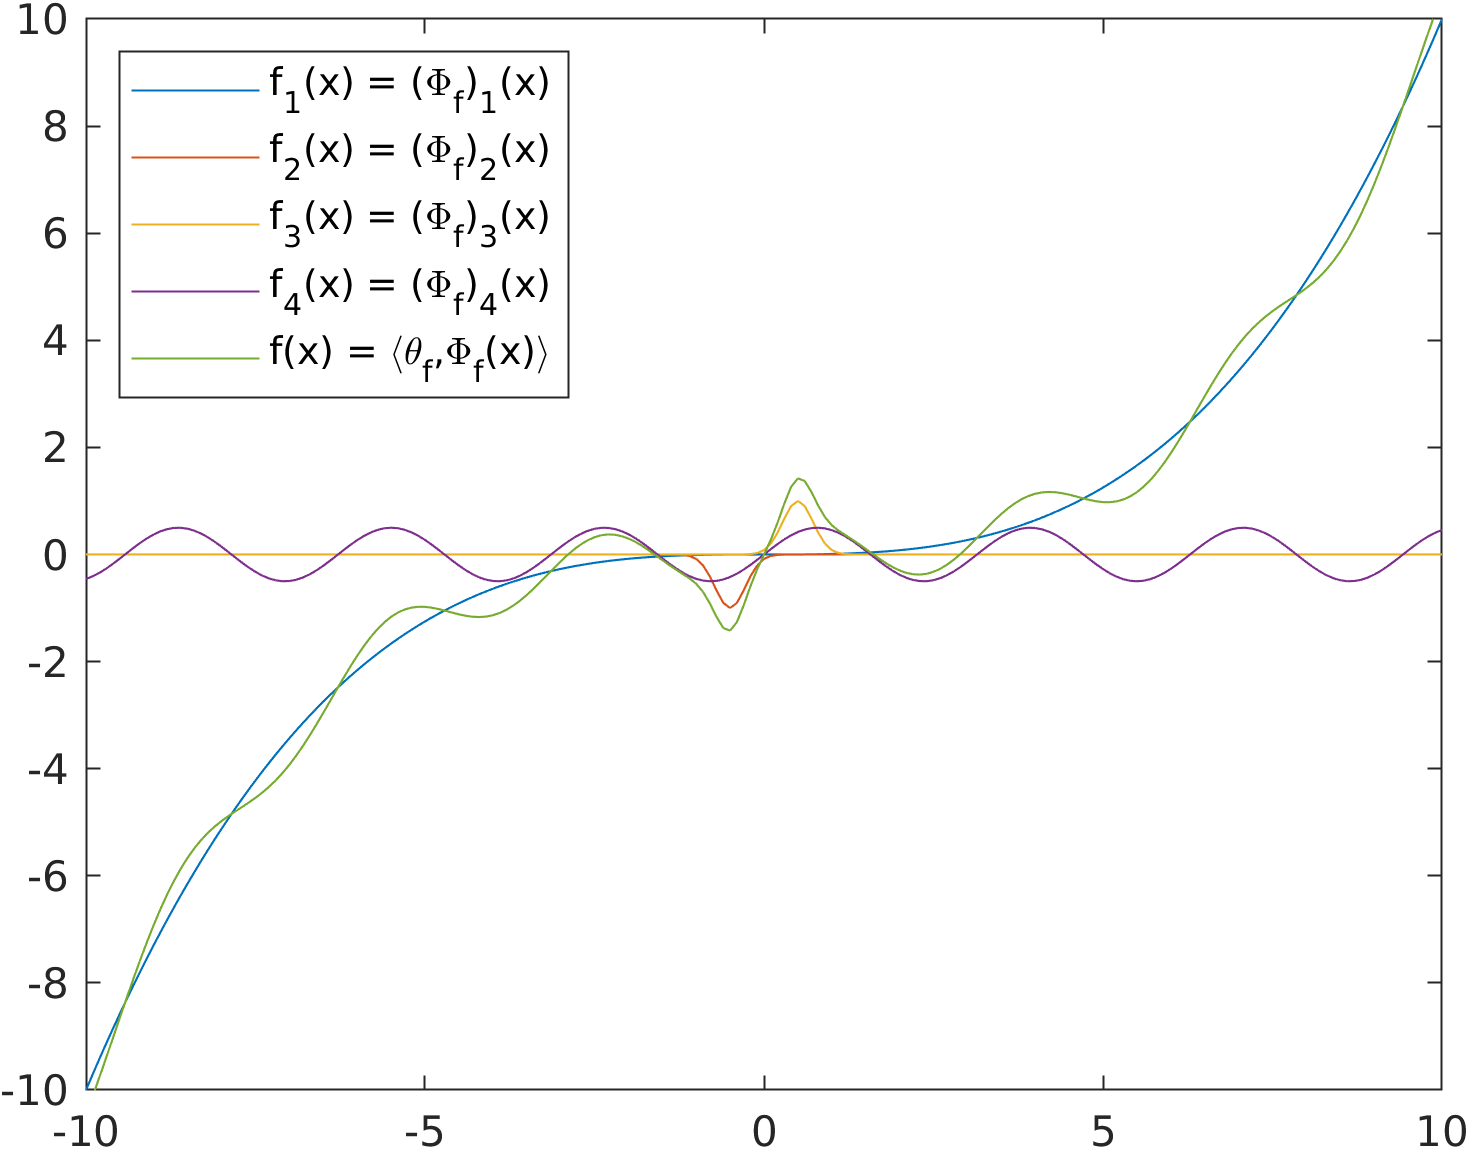
\includegraphics[scale=1.0]{Graphics/Function.png}
		\caption{Nonlinear function $f$}
	\end{figure}

	Here are our simulation results in different time windows:
	
	\begin{figure}[H]
		\centering
		\begin{subfigure}{.45\textwidth}
			\centering
			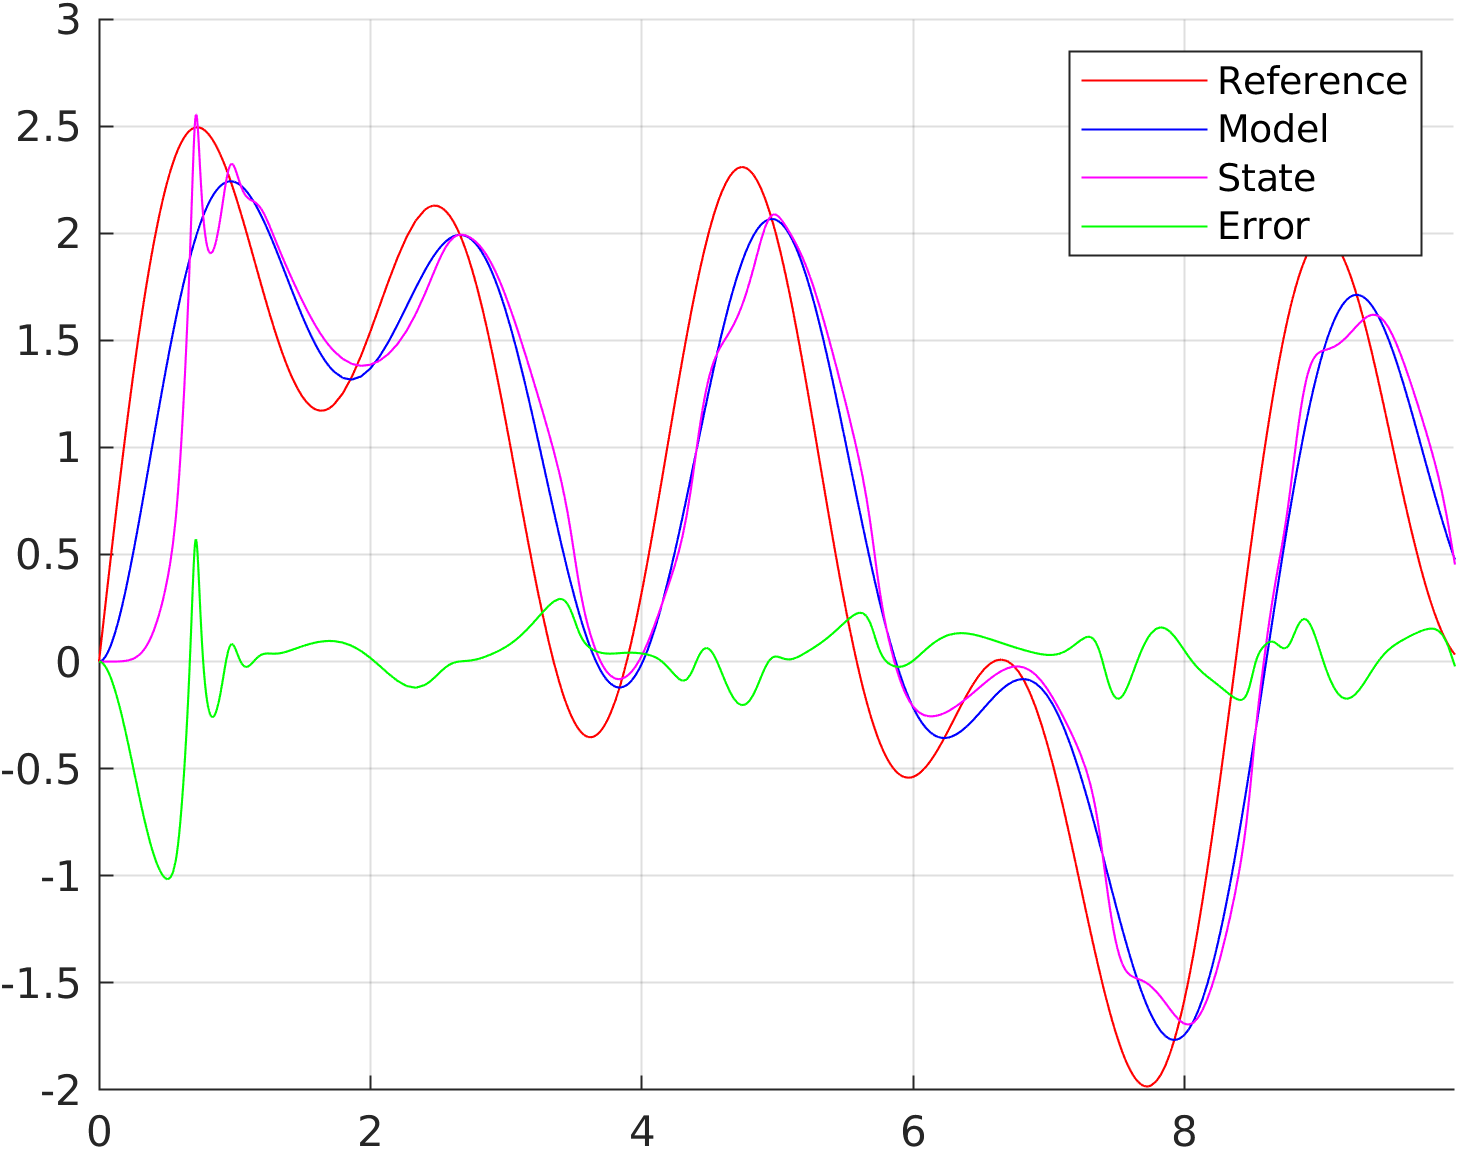
\includegraphics[width=1\textwidth]{Graphics/NonLinearState1.png}
		\end{subfigure}%
		\begin{subfigure}{.45\textwidth}
			\centering
			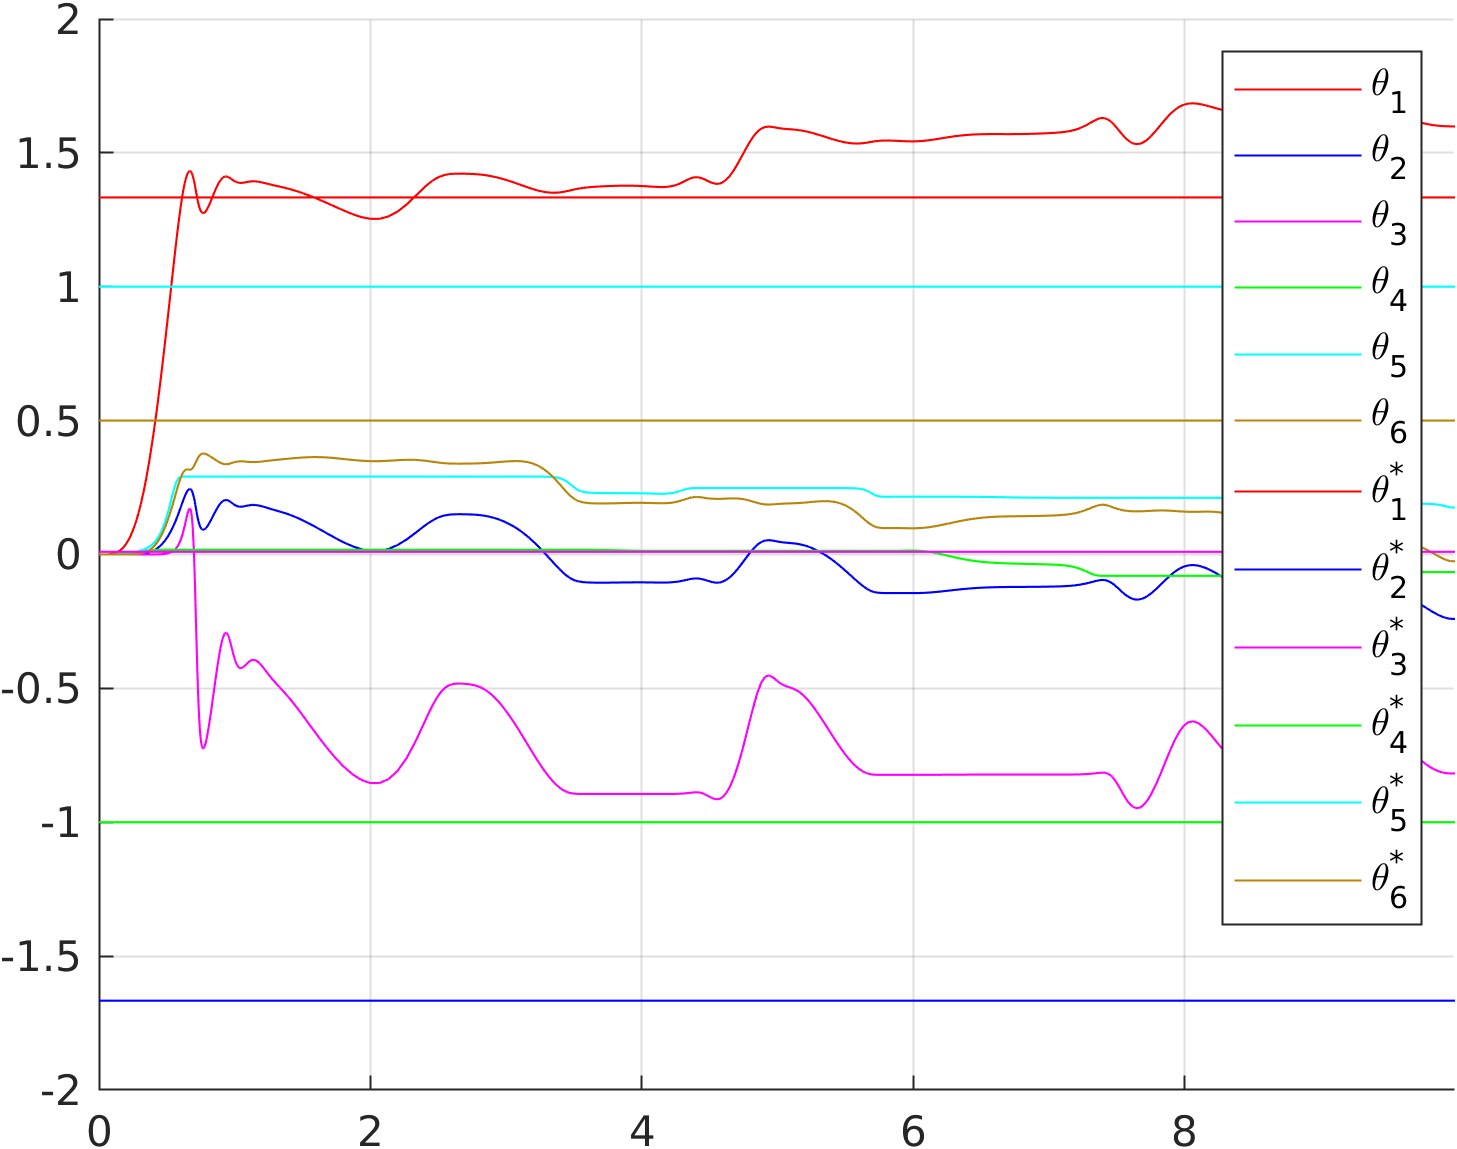
\includegraphics[width=1\textwidth]{Graphics/NonLinearParameters1.png}
		\end{subfigure}
		\begin{subfigure}{.45\textwidth}
			\centering
			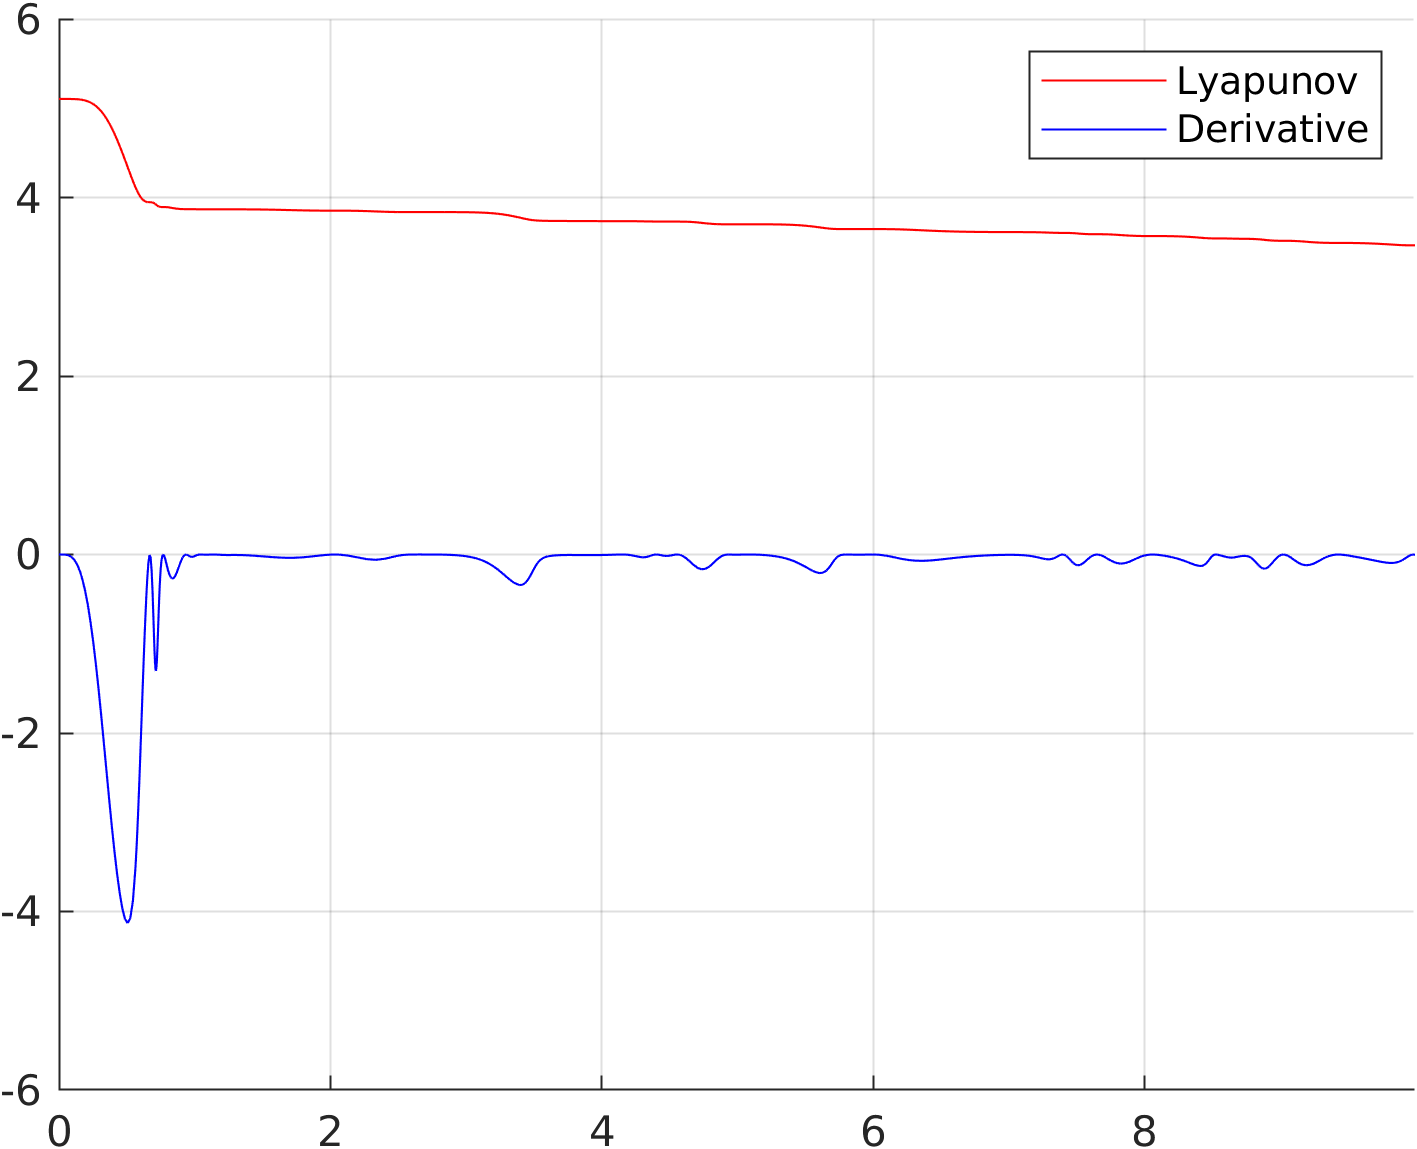
\includegraphics[width=1\textwidth]{Graphics/NonLinearLyapunov1.png}
		\end{subfigure}%
		\begin{subfigure}{.45\textwidth}
			\centering
			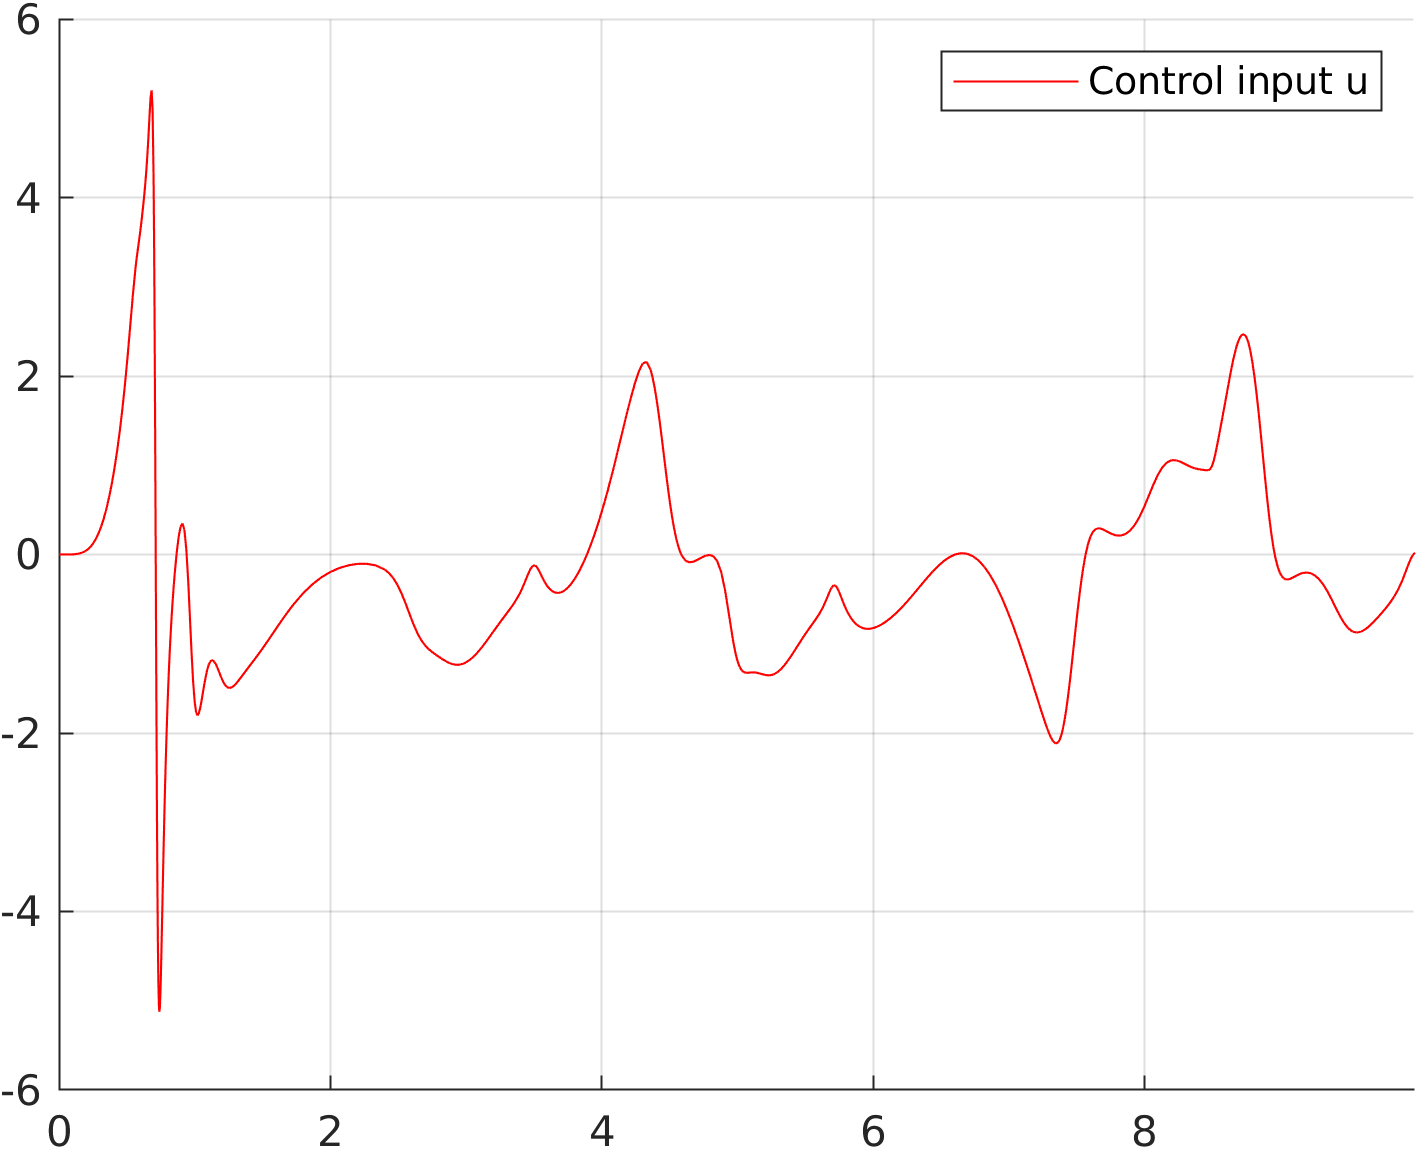
\includegraphics[width=1\textwidth]{Graphics/NonLinearControl1.png}
		\end{subfigure}
		\caption{$t \in [0,10]s$}
	\end{figure}

	\begin{figure}[H]
		\centering
		\begin{subfigure}{.45\textwidth}
			\centering
			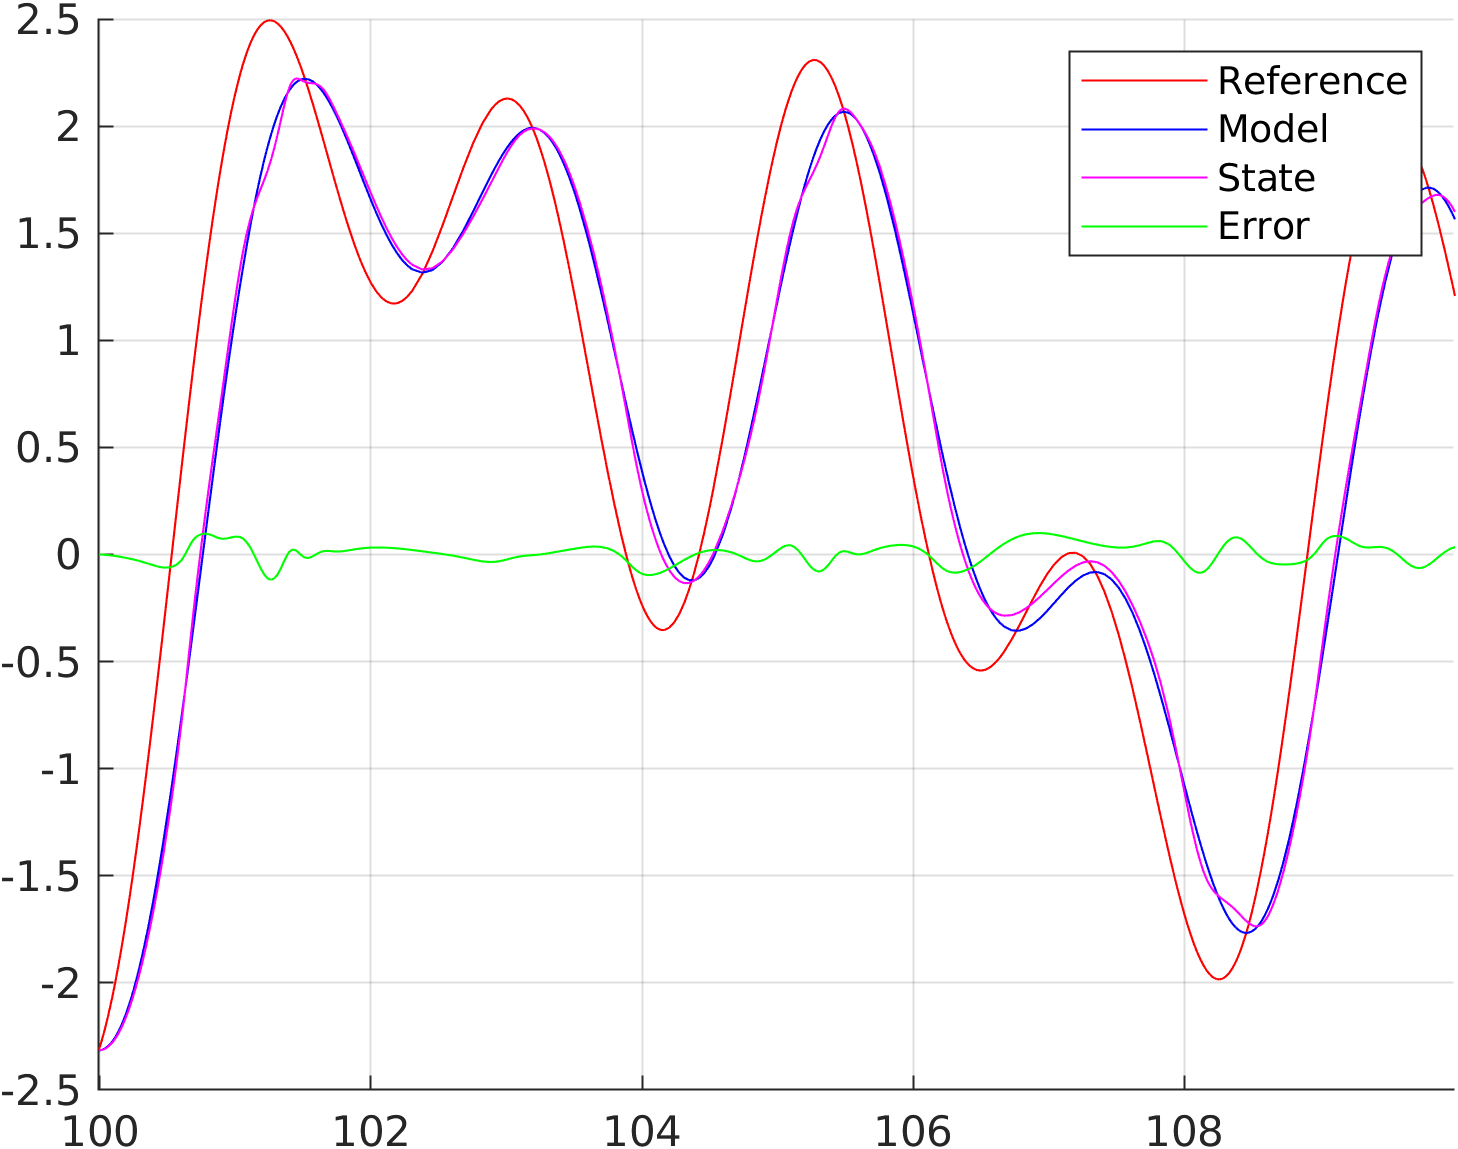
\includegraphics[width=1\textwidth]{Graphics/NonLinearState2.png}
		\end{subfigure}%
		\begin{subfigure}{.45\textwidth}
			\centering
			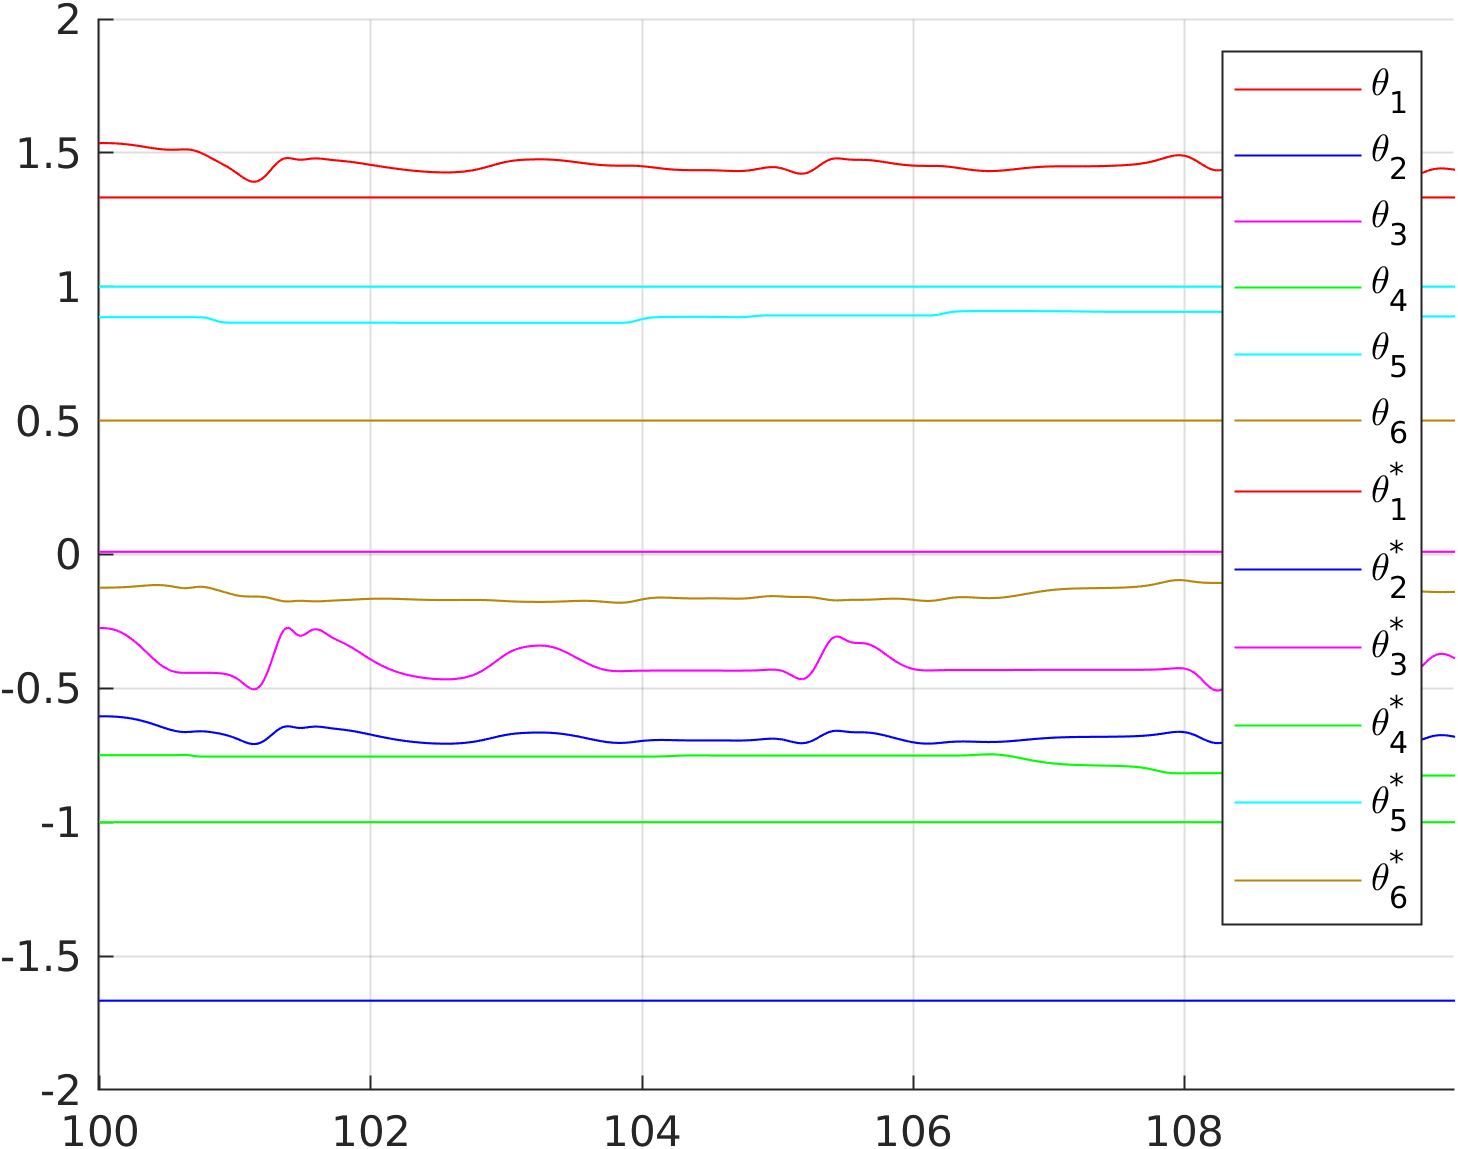
\includegraphics[width=1\textwidth]{Graphics/NonLinearParameters2.png}
		\end{subfigure}
		\begin{subfigure}{.45\textwidth}
			\centering
			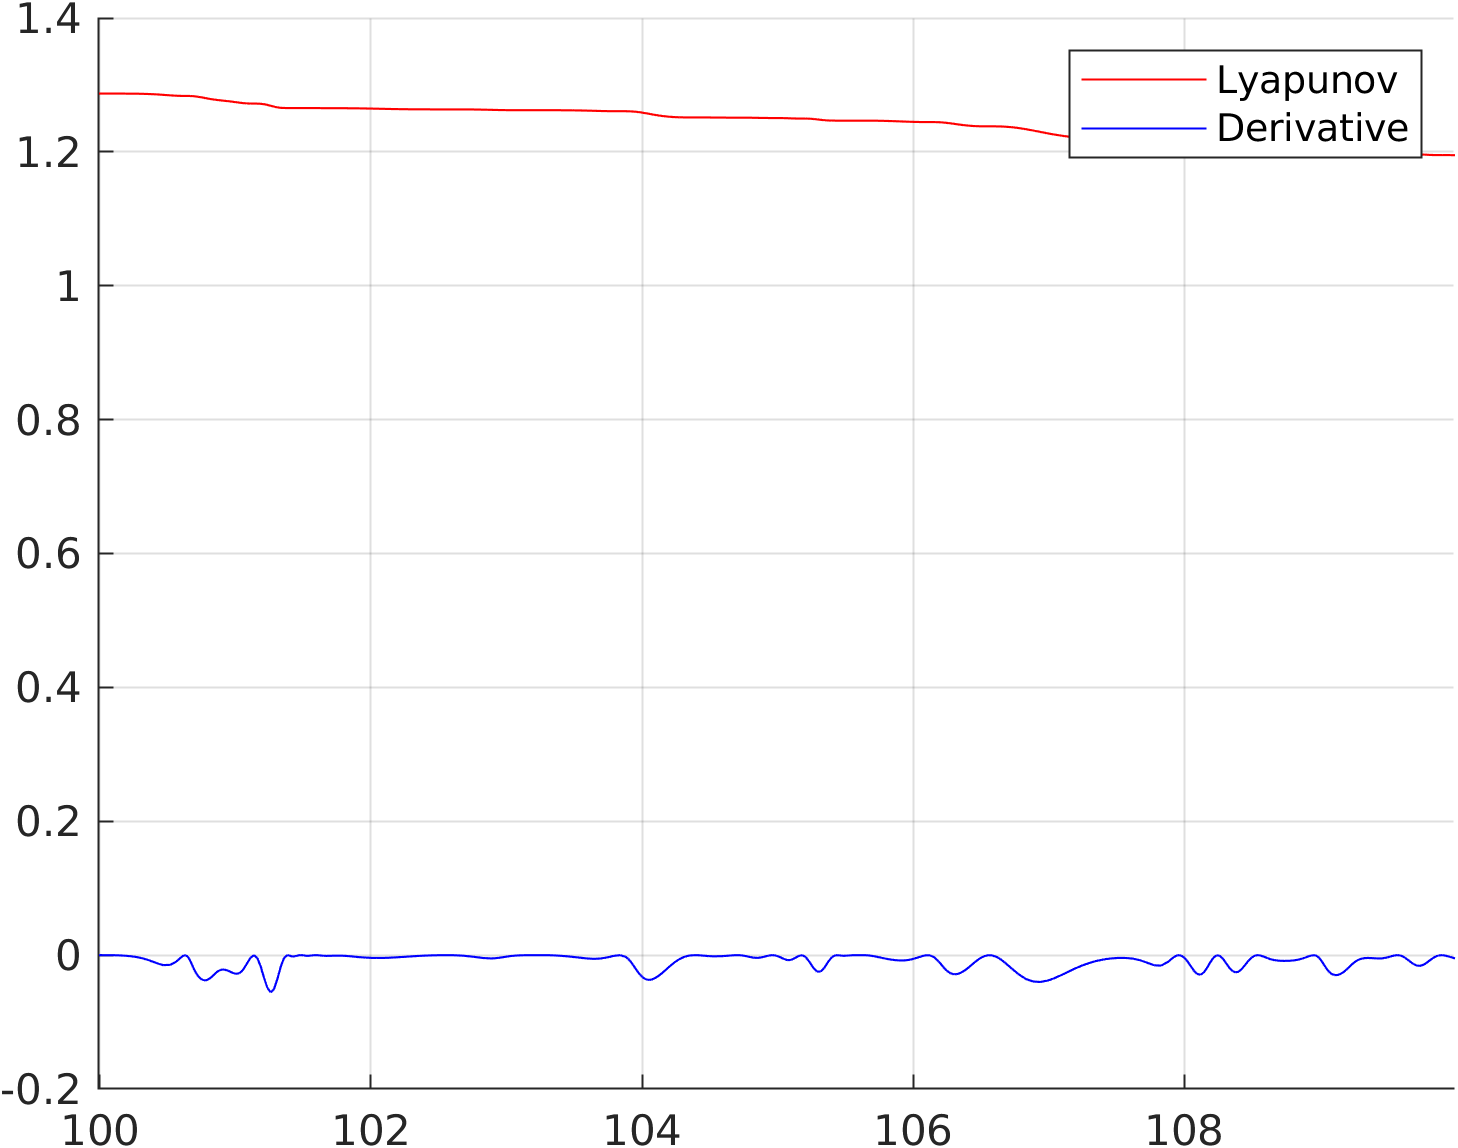
\includegraphics[width=1\textwidth]{Graphics/NonLinearLyapunov2.png}
		\end{subfigure}%
		\begin{subfigure}{.45\textwidth}
			\centering
			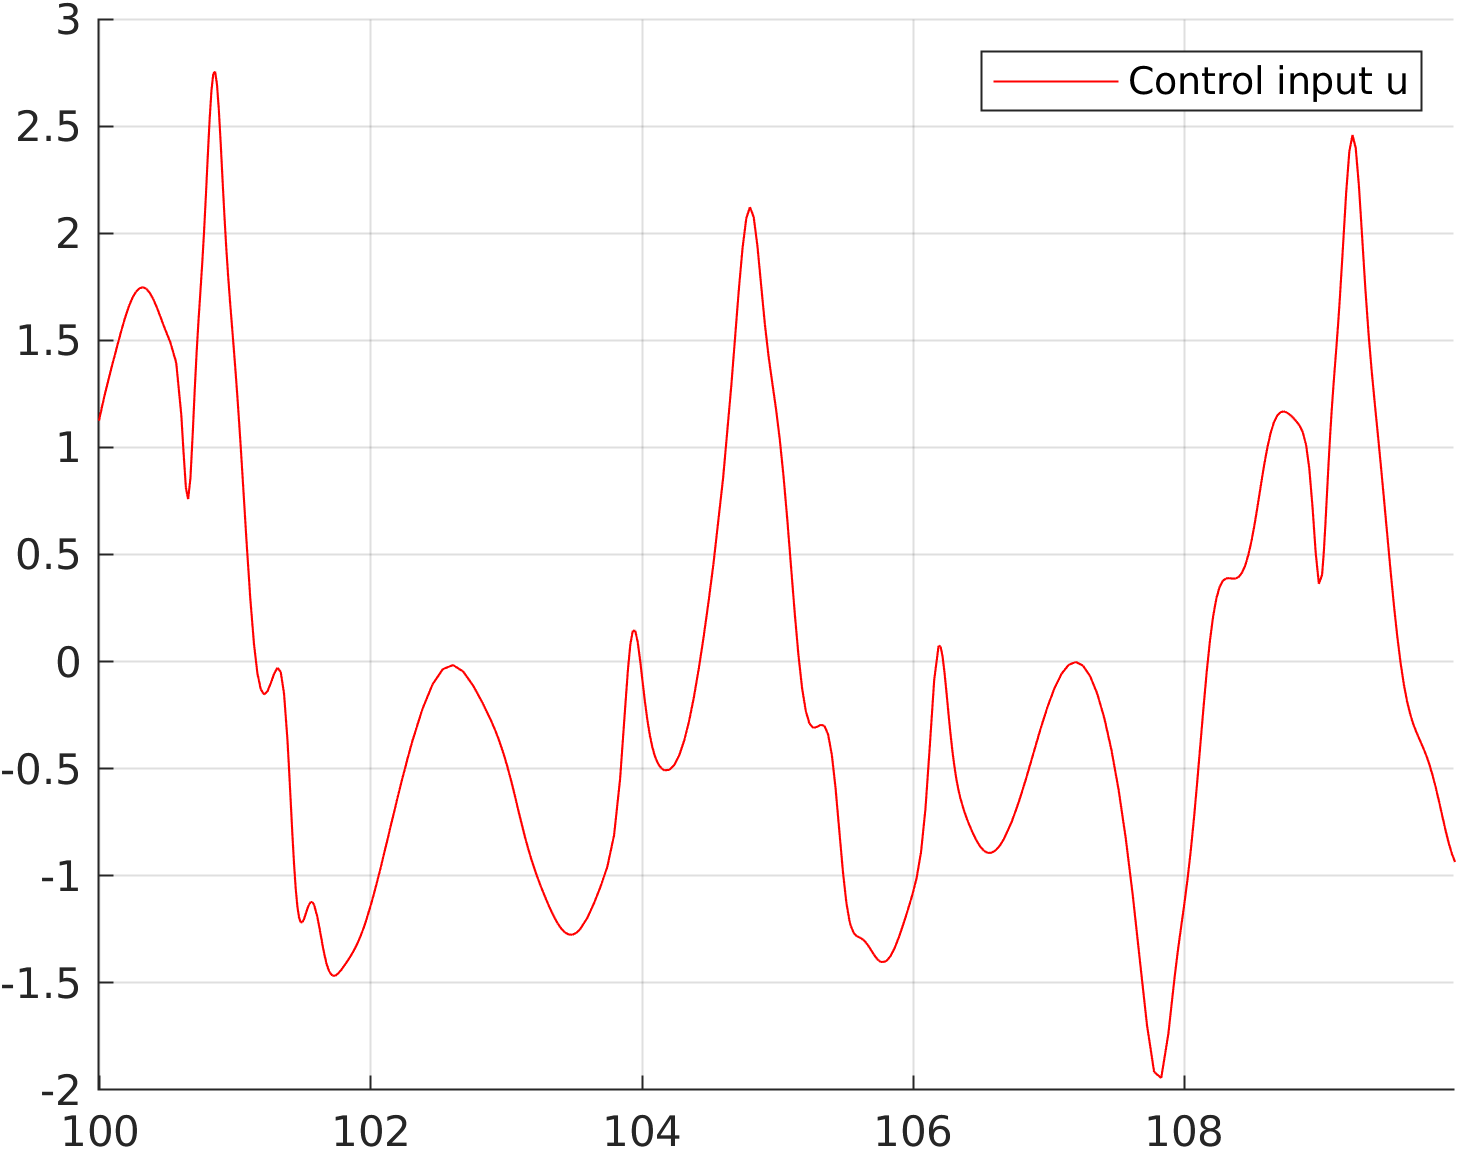
\includegraphics[width=1\textwidth]{Graphics/NonLinearControl2.png}
		\end{subfigure}
		\caption{$t \in [100,110]s$}
	\end{figure}

	\begin{figure}[H]
		\centering
		\begin{subfigure}{.45\textwidth}
			\centering
			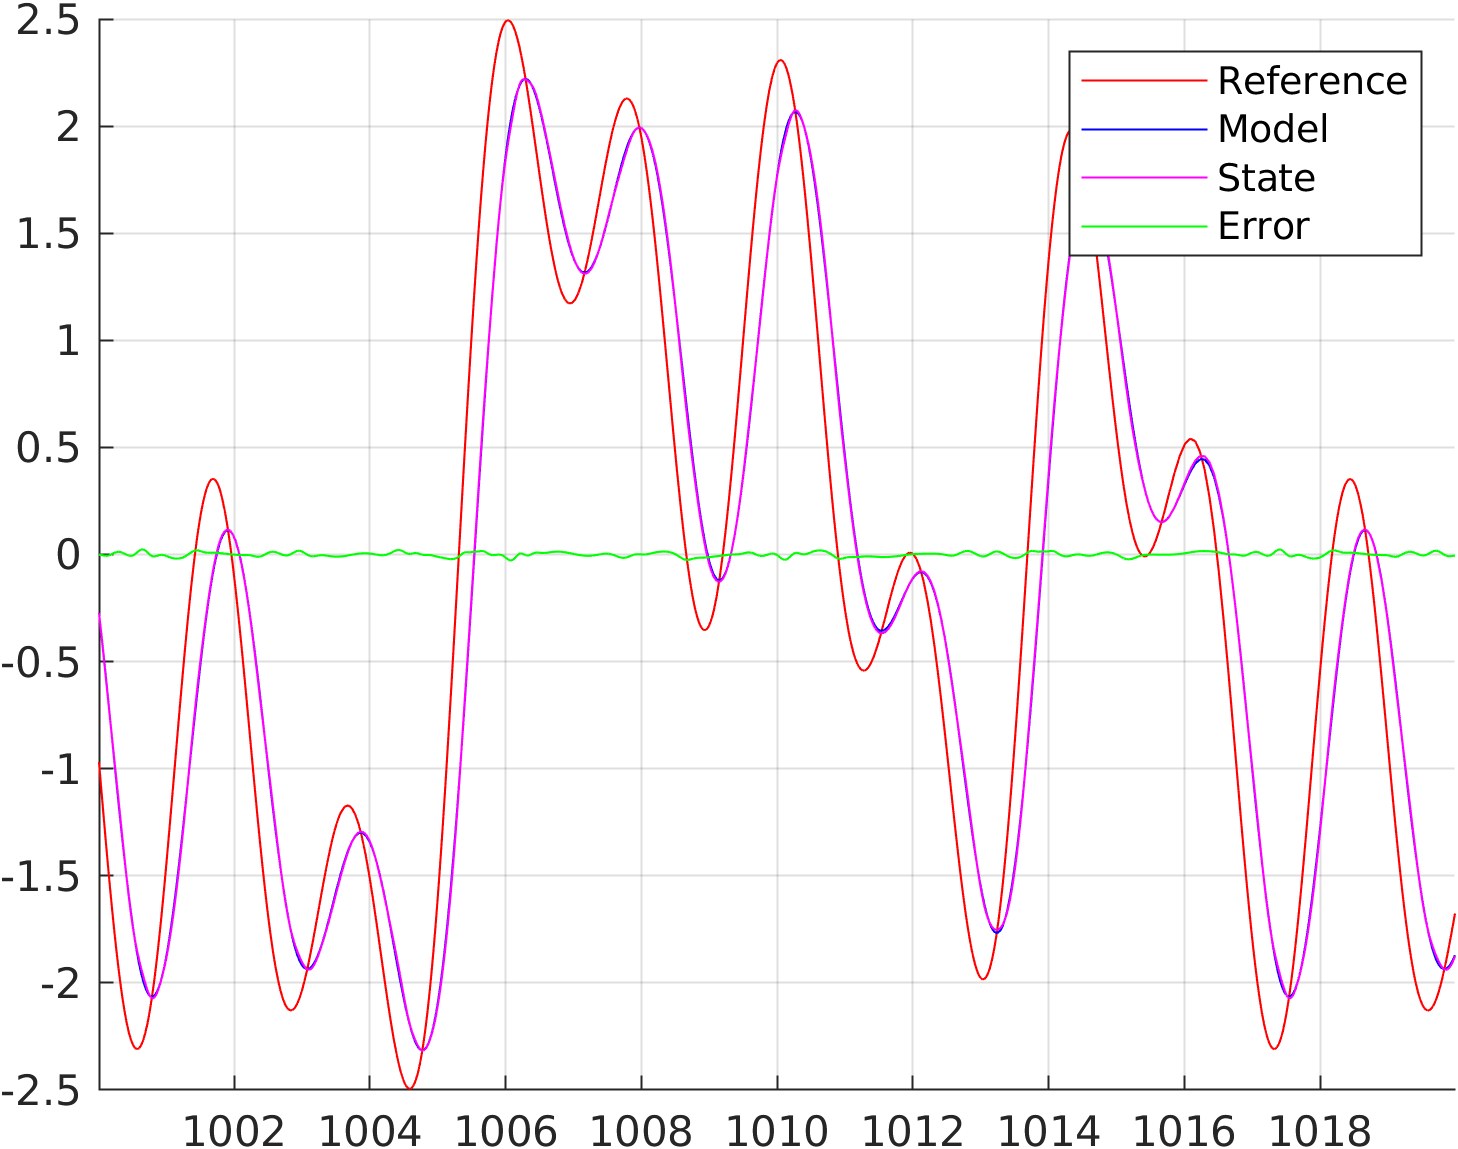
\includegraphics[width=1\textwidth]{Graphics/NonLinearState3.png}
		\end{subfigure}%
		\begin{subfigure}{.45\textwidth}
			\centering
			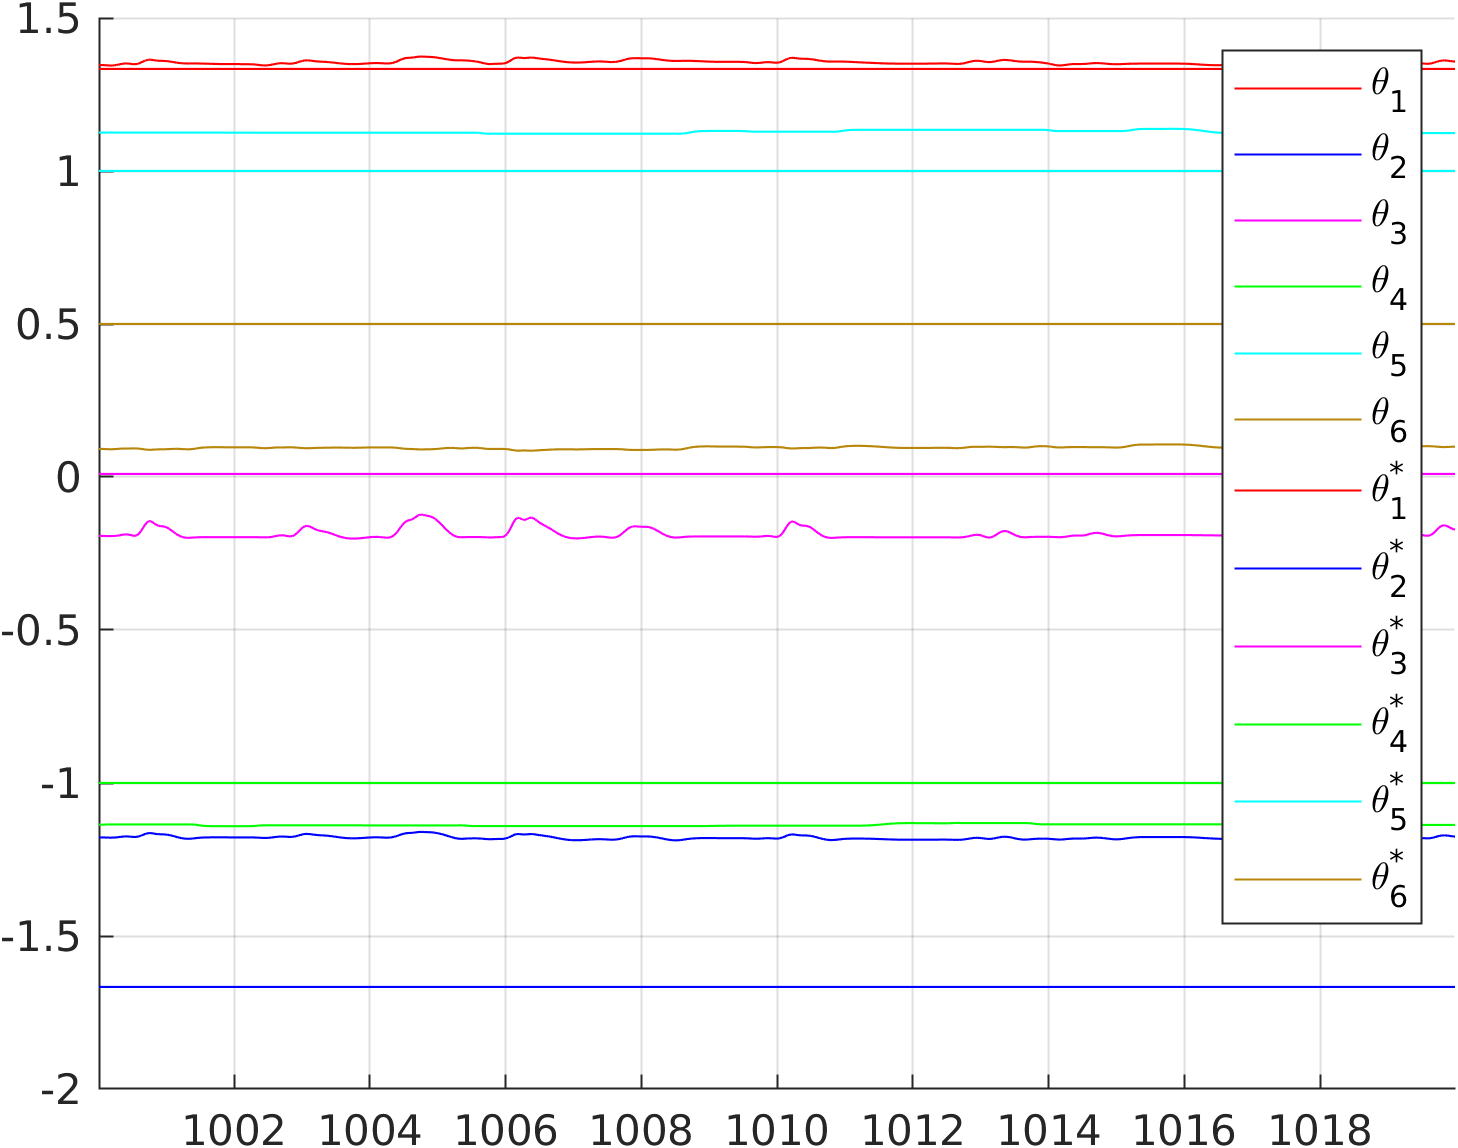
\includegraphics[width=1\textwidth]{Graphics/NonLinearParameters3.png}
		\end{subfigure}
		\begin{subfigure}{.45\textwidth}
			\centering
			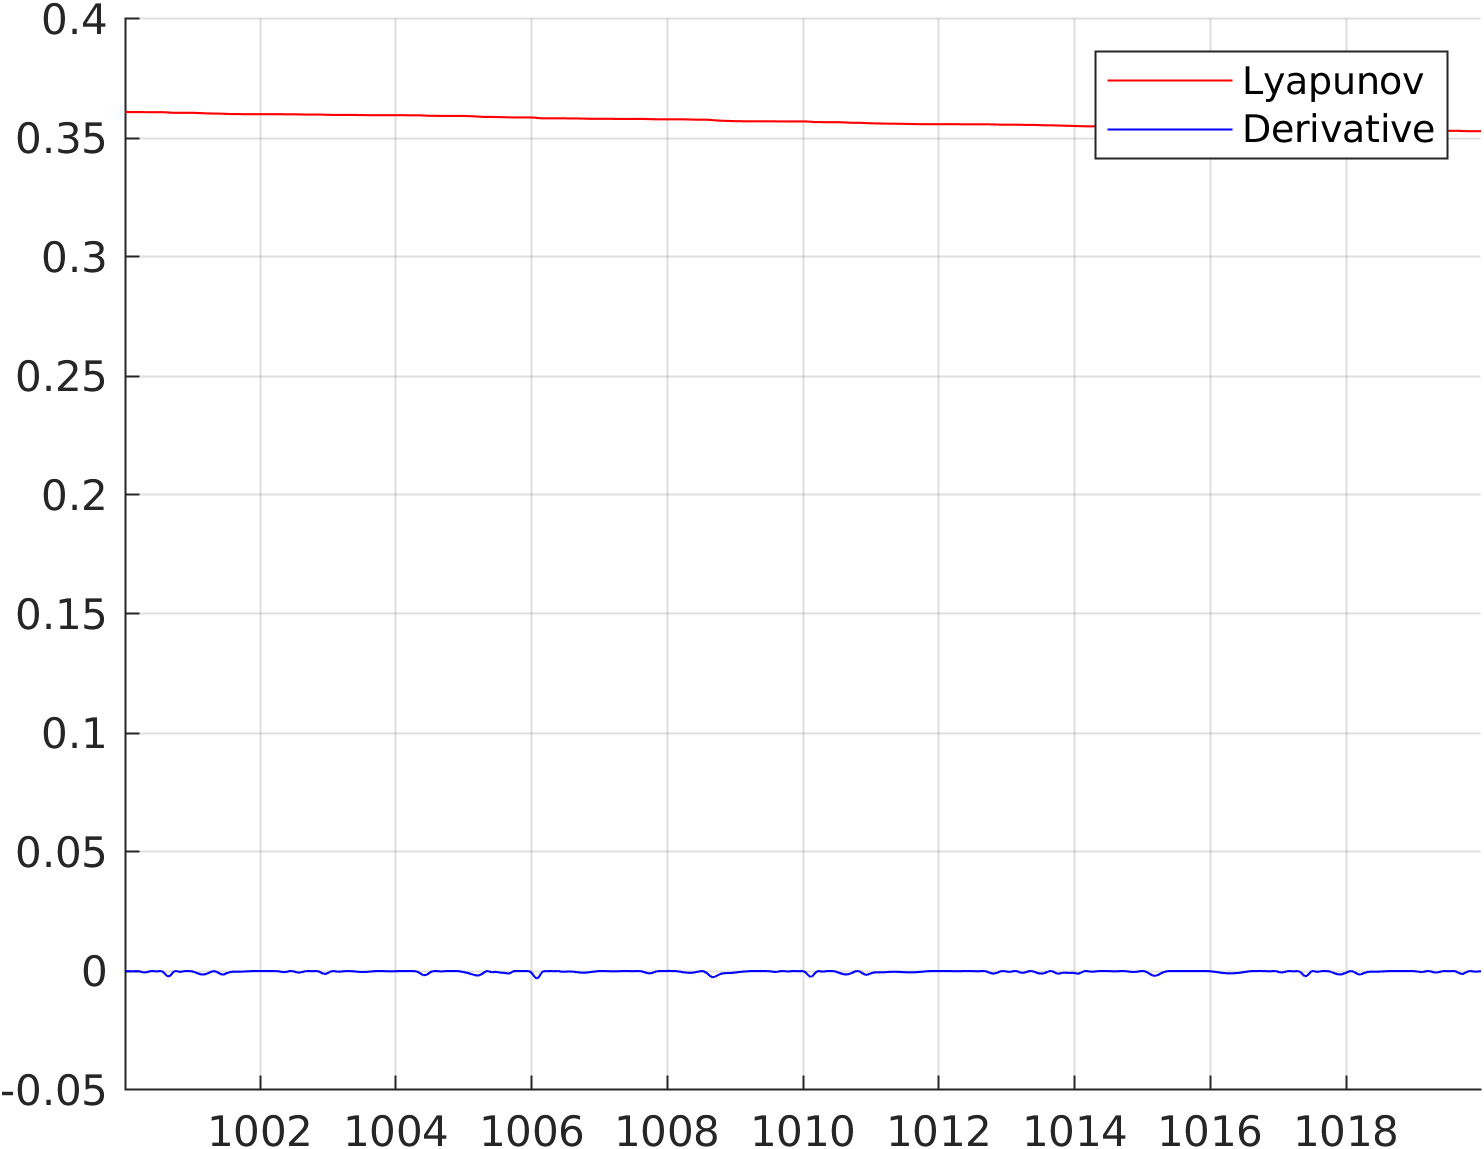
\includegraphics[width=1\textwidth]{Graphics/NonLinearLyapunov3.png}
		\end{subfigure}%
		\begin{subfigure}{.45\textwidth}
			\centering
			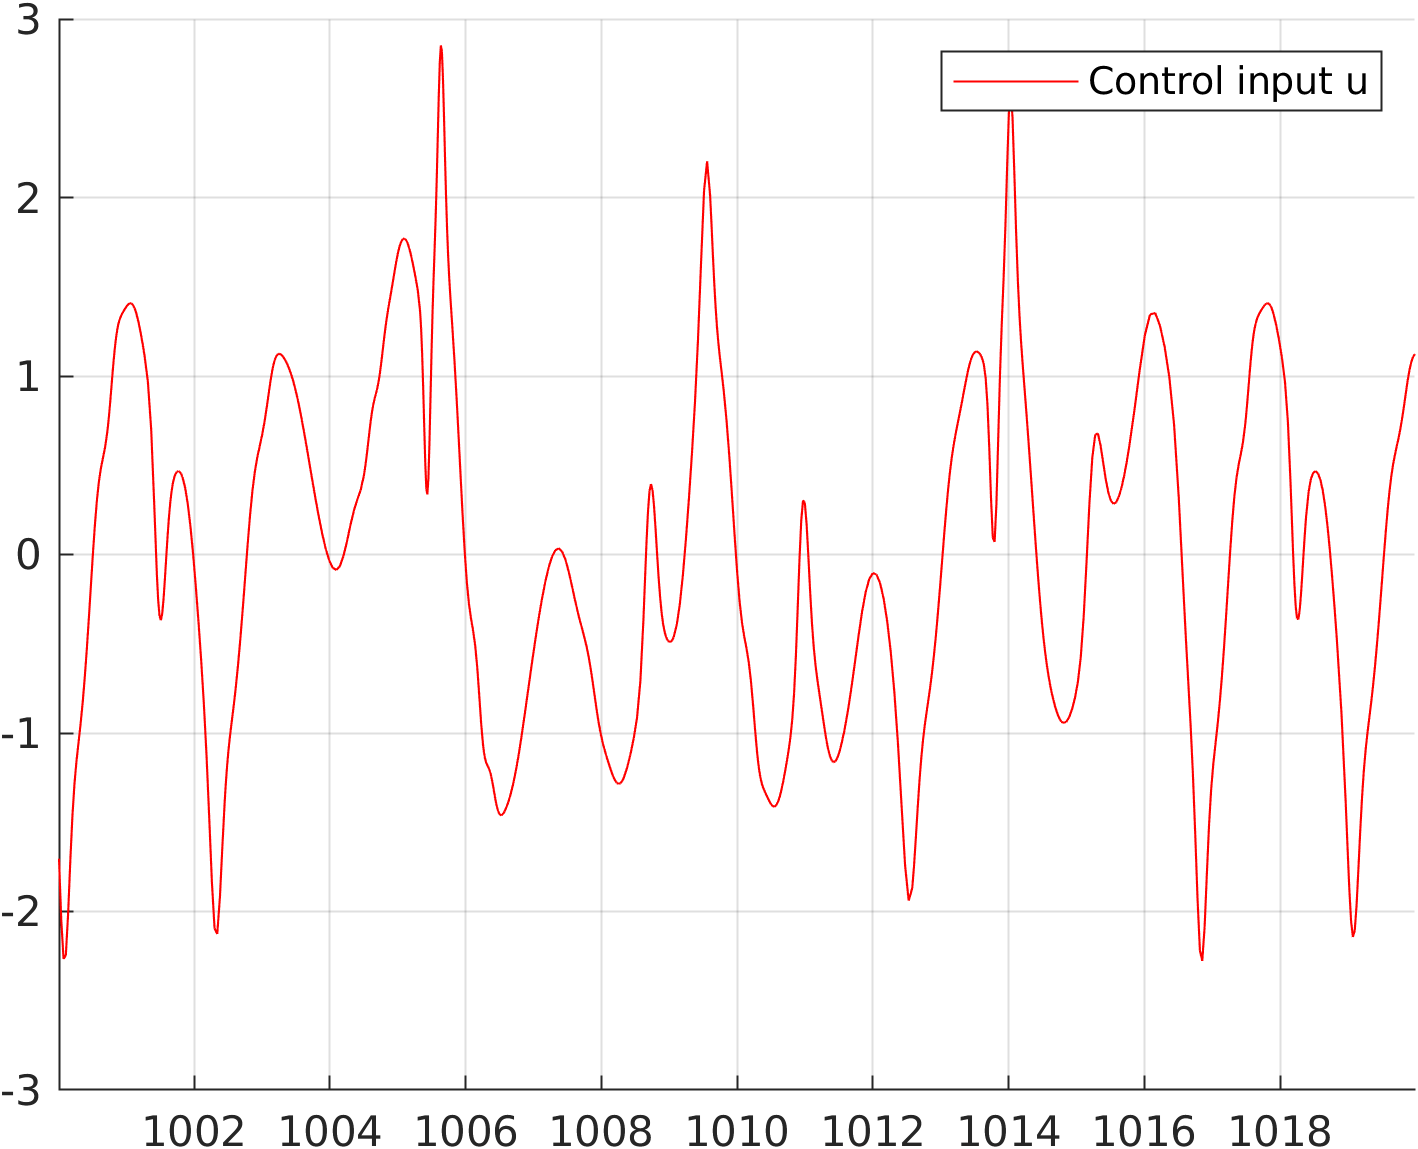
\includegraphics[width=1\textwidth]{Graphics/NonLinearControl3.png}
		\end{subfigure}
		\caption{$t \in [1000,1020]s$}
	\end{figure}

	\begin{figure}[H]
		\centering
		\begin{subfigure}{.45\textwidth}
			\centering
			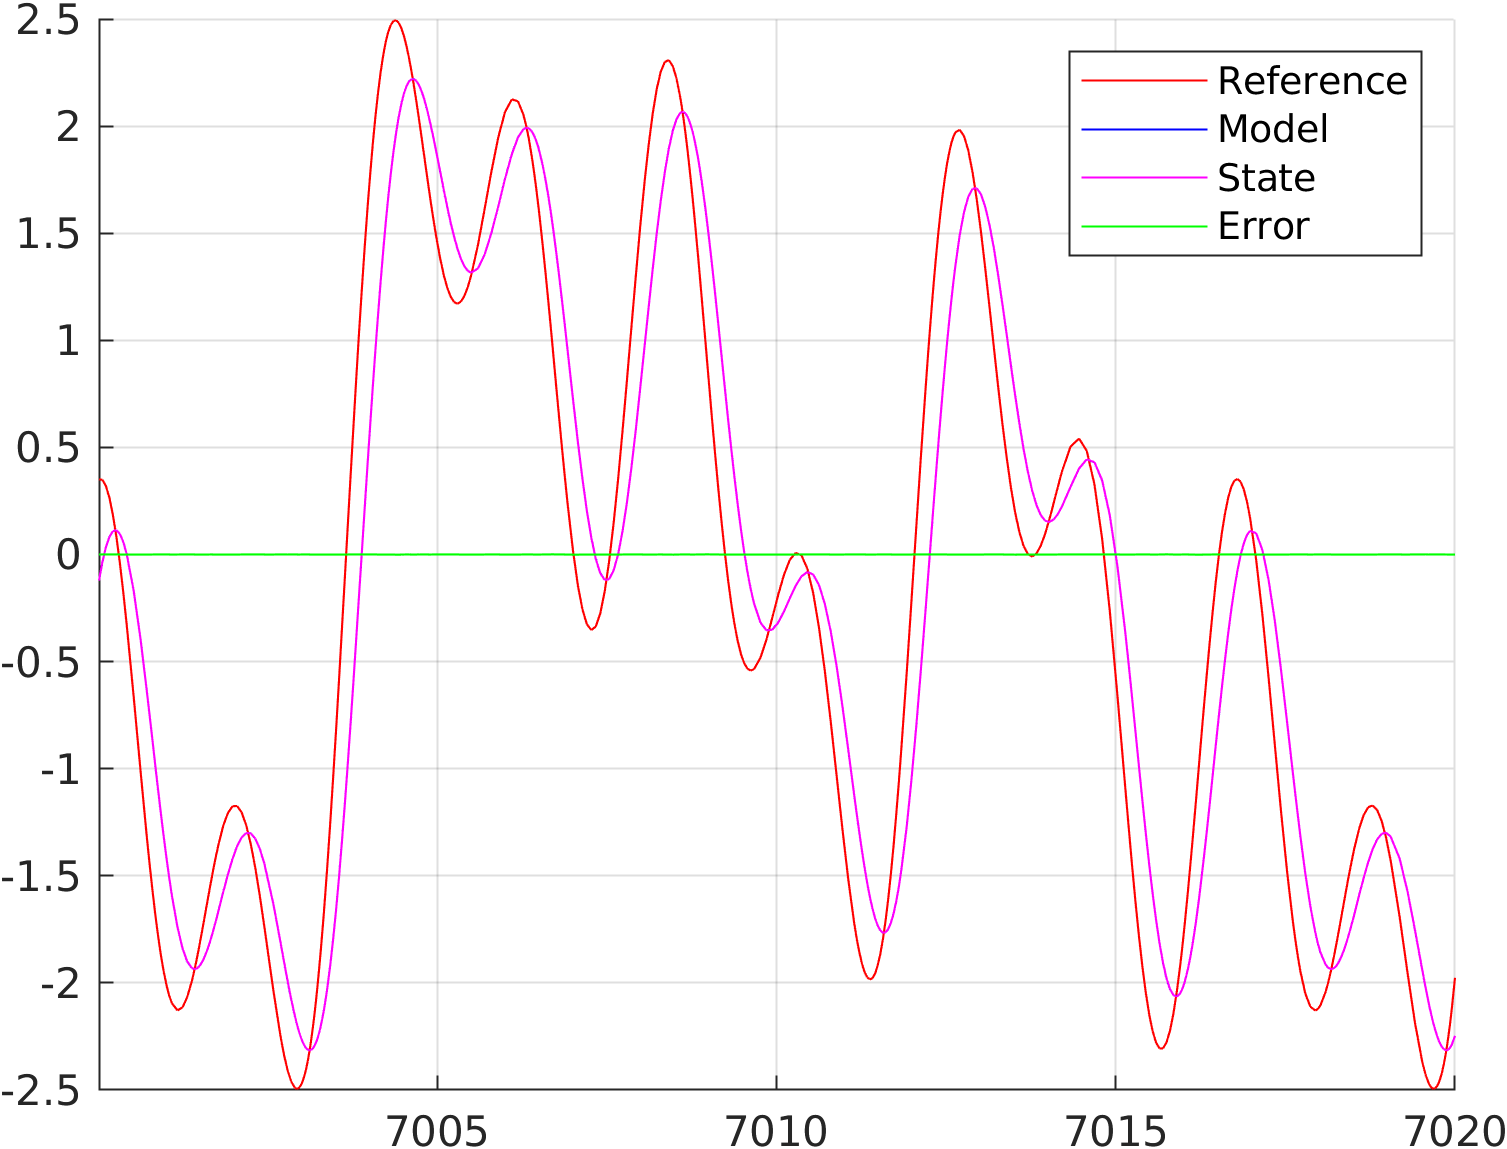
\includegraphics[width=1\textwidth]{Graphics/NonLinearState4.png}
		\end{subfigure}%
		\begin{subfigure}{.45\textwidth}
			\centering
			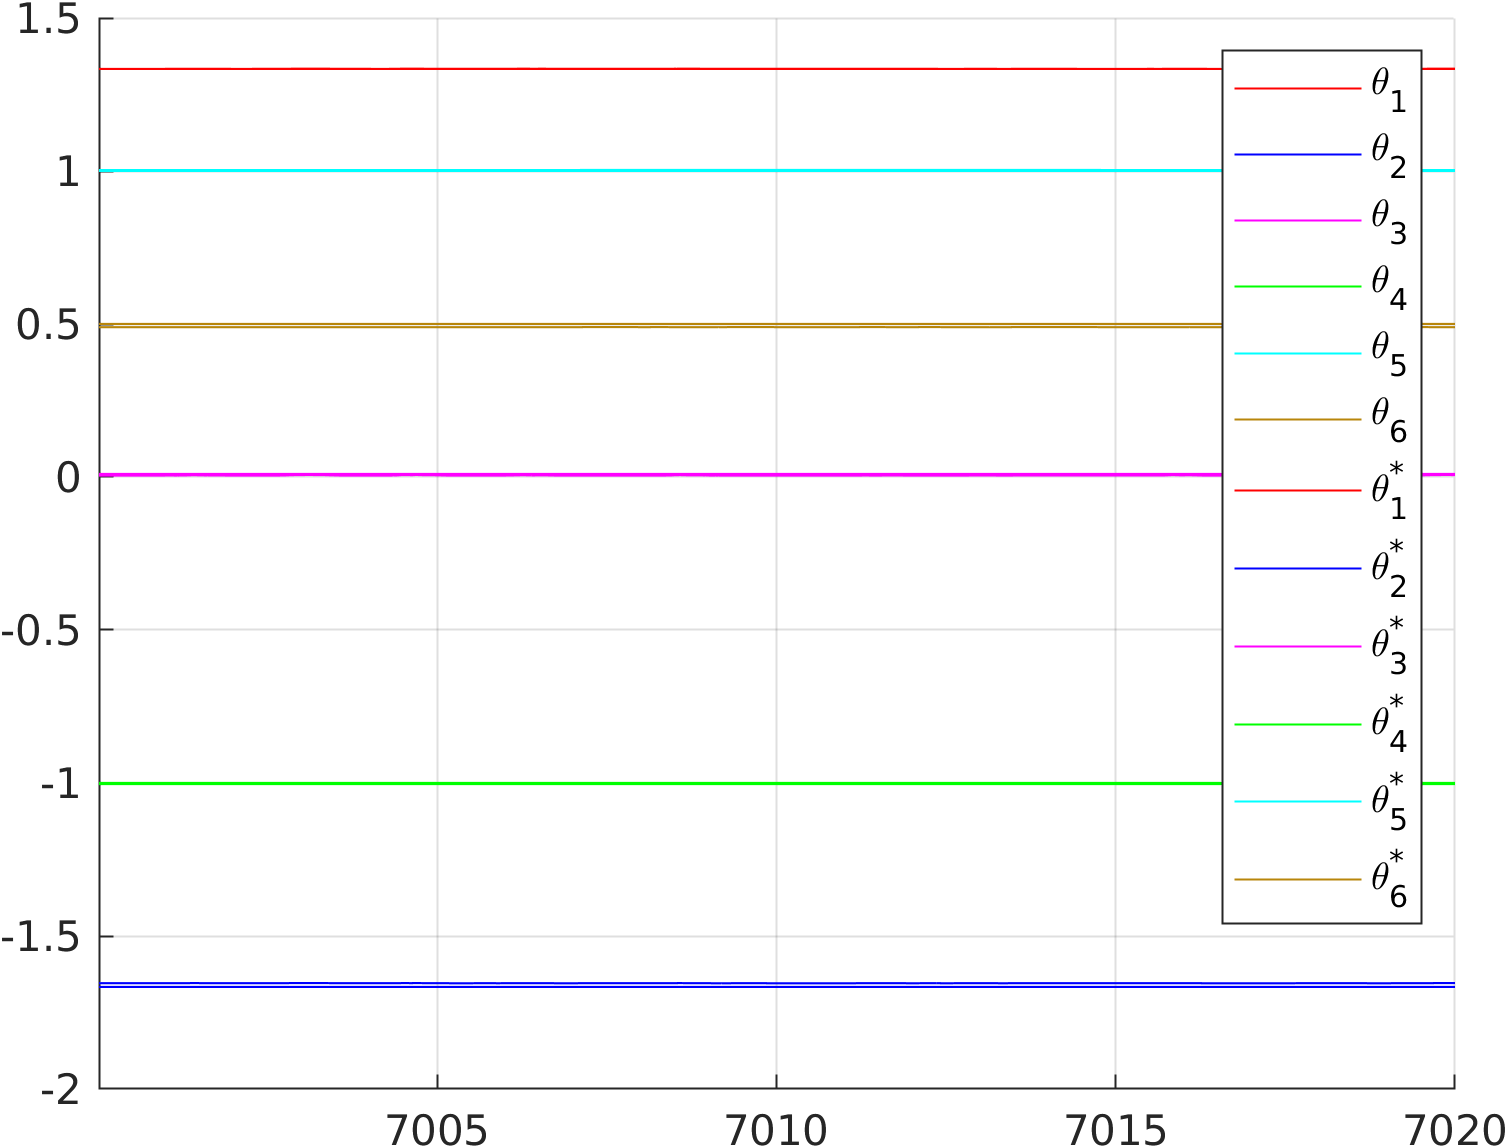
\includegraphics[width=1\textwidth]{Graphics/NonLinearParameters4.png}
		\end{subfigure}
		\begin{subfigure}{.45\textwidth}
			\centering
			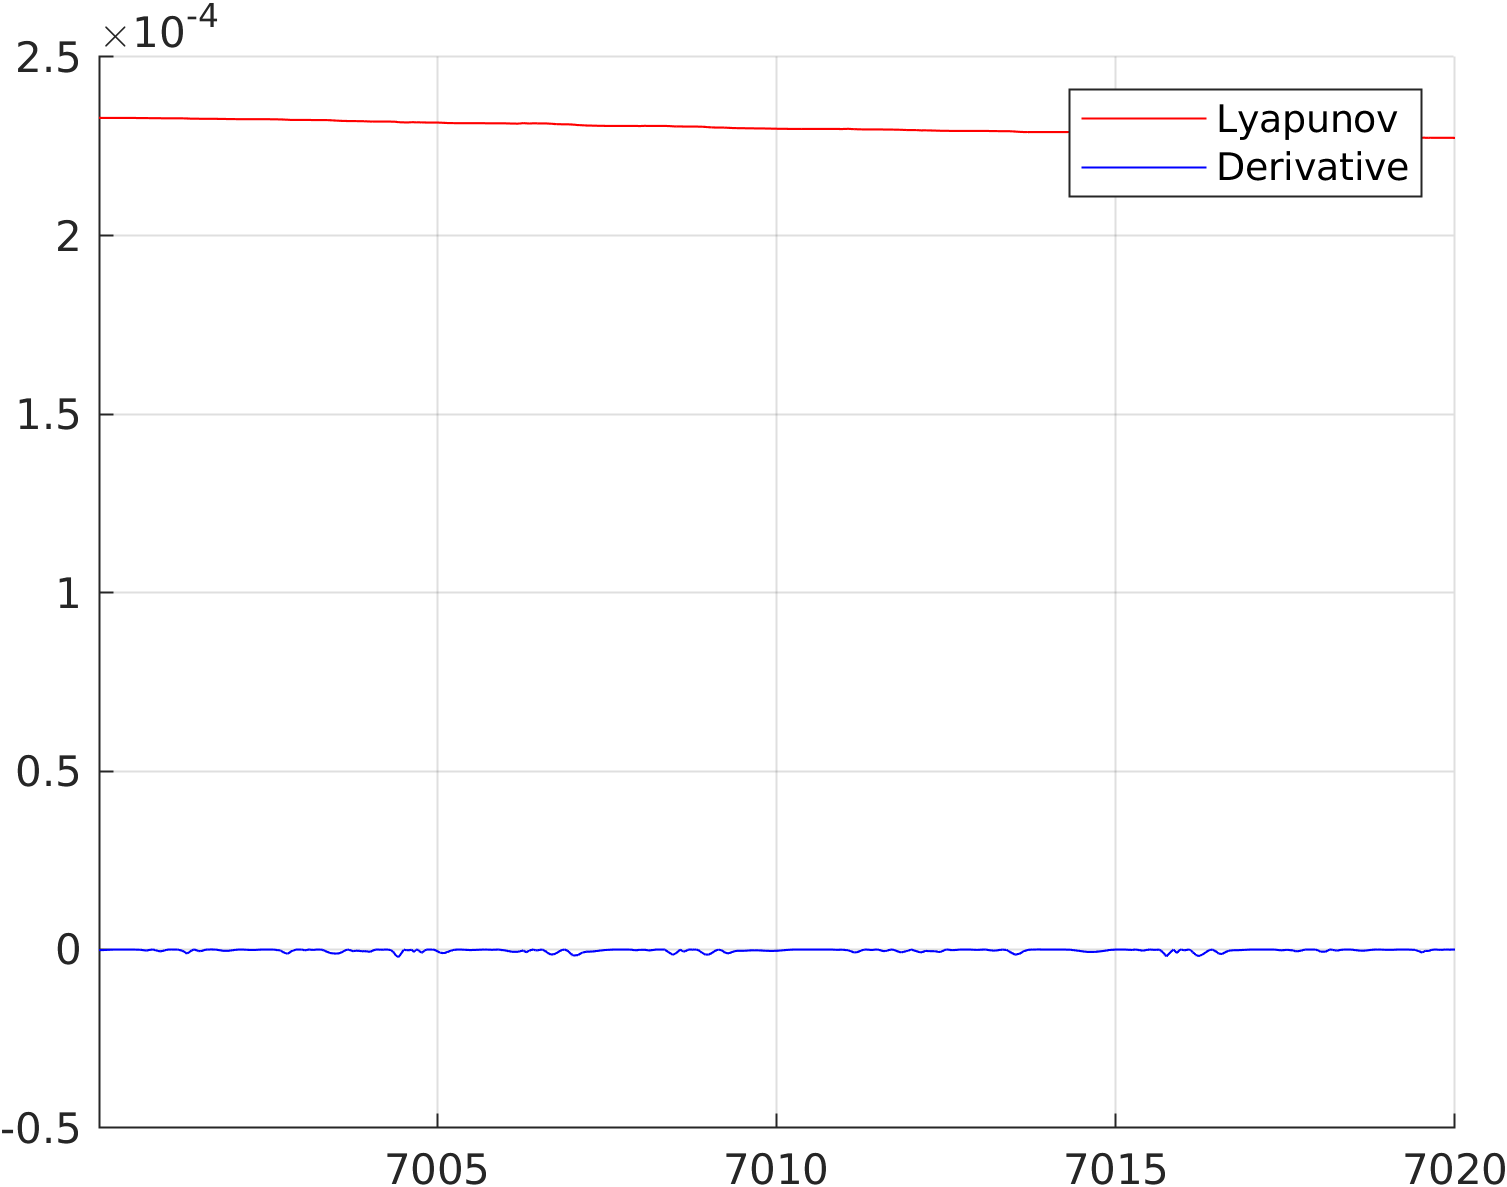
\includegraphics[width=1\textwidth]{Graphics/NonLinearLyapunov4.png}
		\end{subfigure}%
		\begin{subfigure}{.45\textwidth}
			\centering
			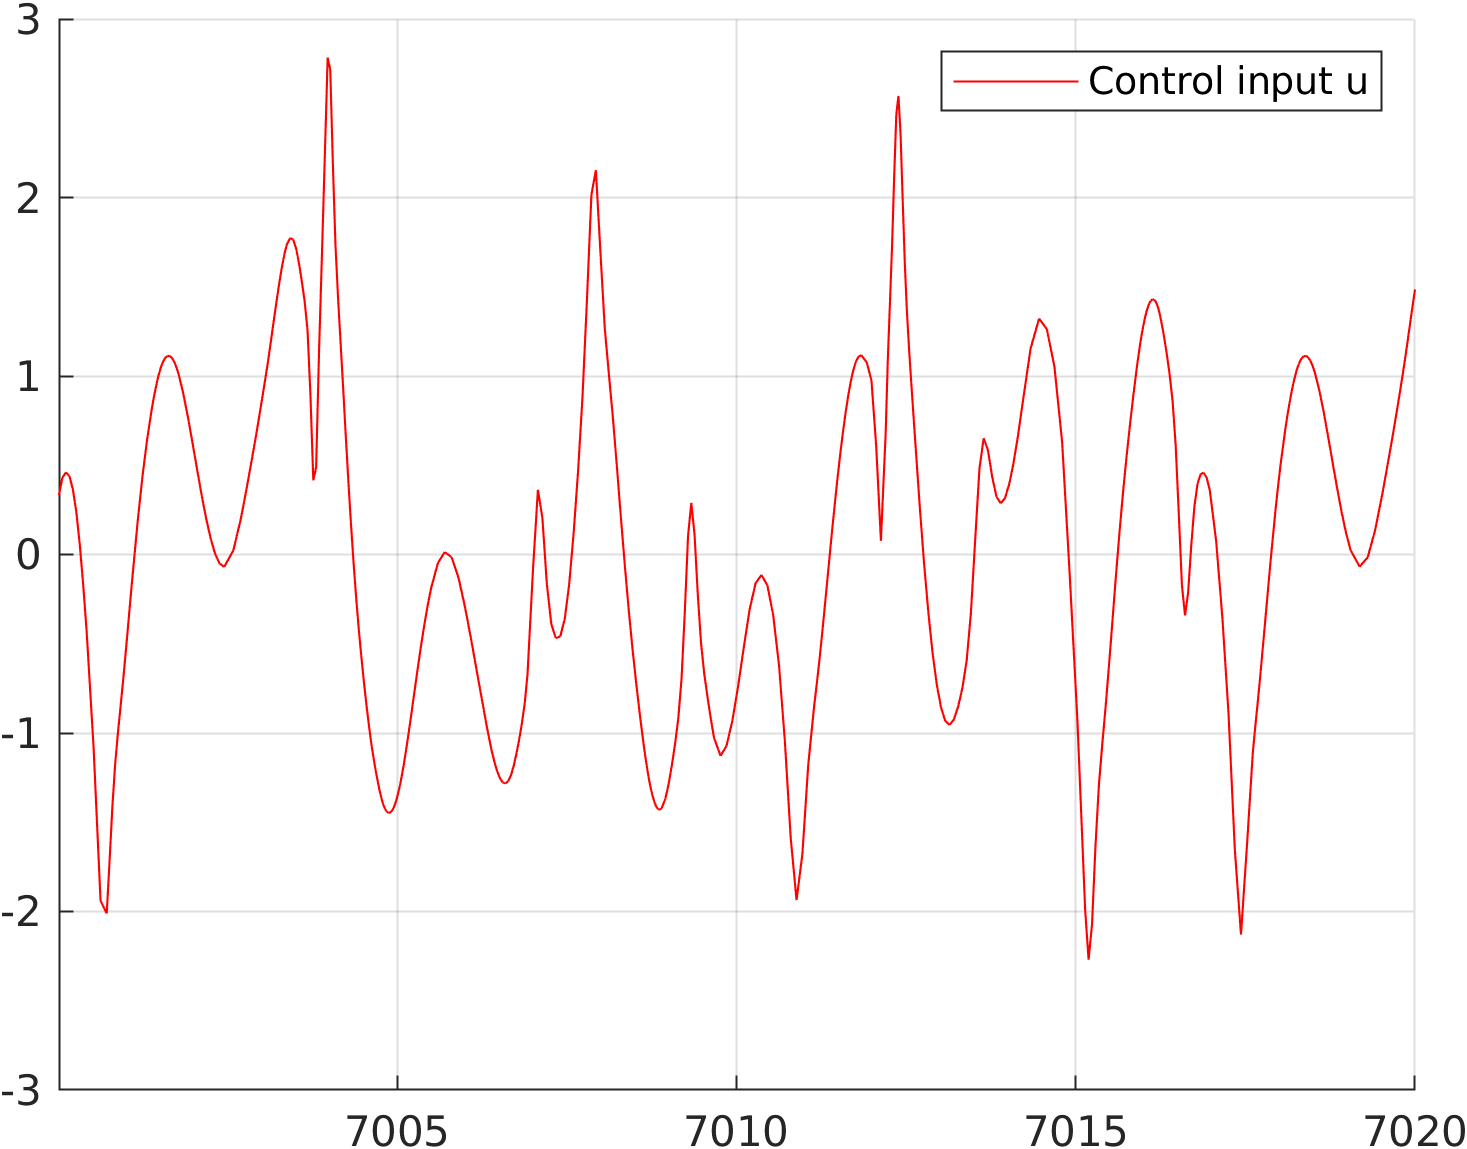
\includegraphics[width=1\textwidth]{Graphics/NonLinearControl4.png}
		\end{subfigure}
		\caption{$t \in [7000,7020]s$}
	\end{figure}
	
	We observe that the parameters eventually converge to their true values, although it takes quite a long time. 
	The tracking of the reference model is already very good for approximately $t \geq 1000s$, but the parameters need approximately $7000s$ to get satisfactory close to their true values.
	
	\subsubsection*{Two parameters known to vanish}
	If we look at the case where two of the parameters are known to be $0$, we have much faster learning:
	
	\begin{figure}[H]
		\centering
		\begin{subfigure}{.45\textwidth}
			\centering
			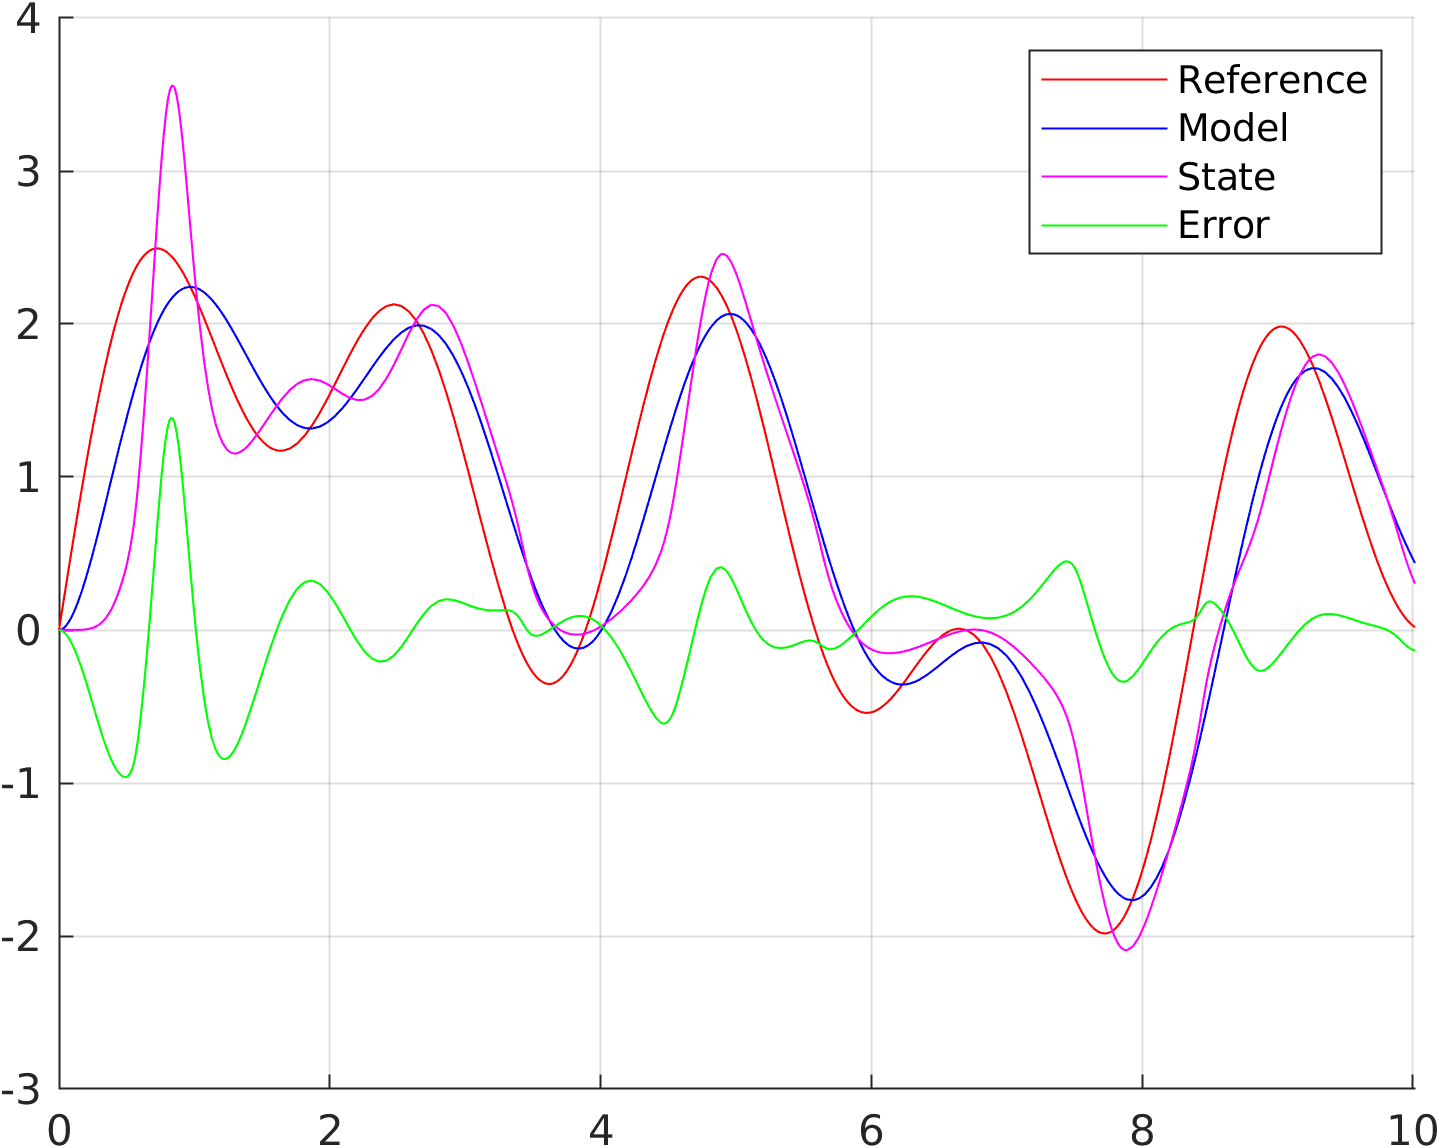
\includegraphics[width=1\textwidth]{Graphics/NonLinearStateZero1.png}
		\end{subfigure}%
		\begin{subfigure}{.45\textwidth}
			\centering
			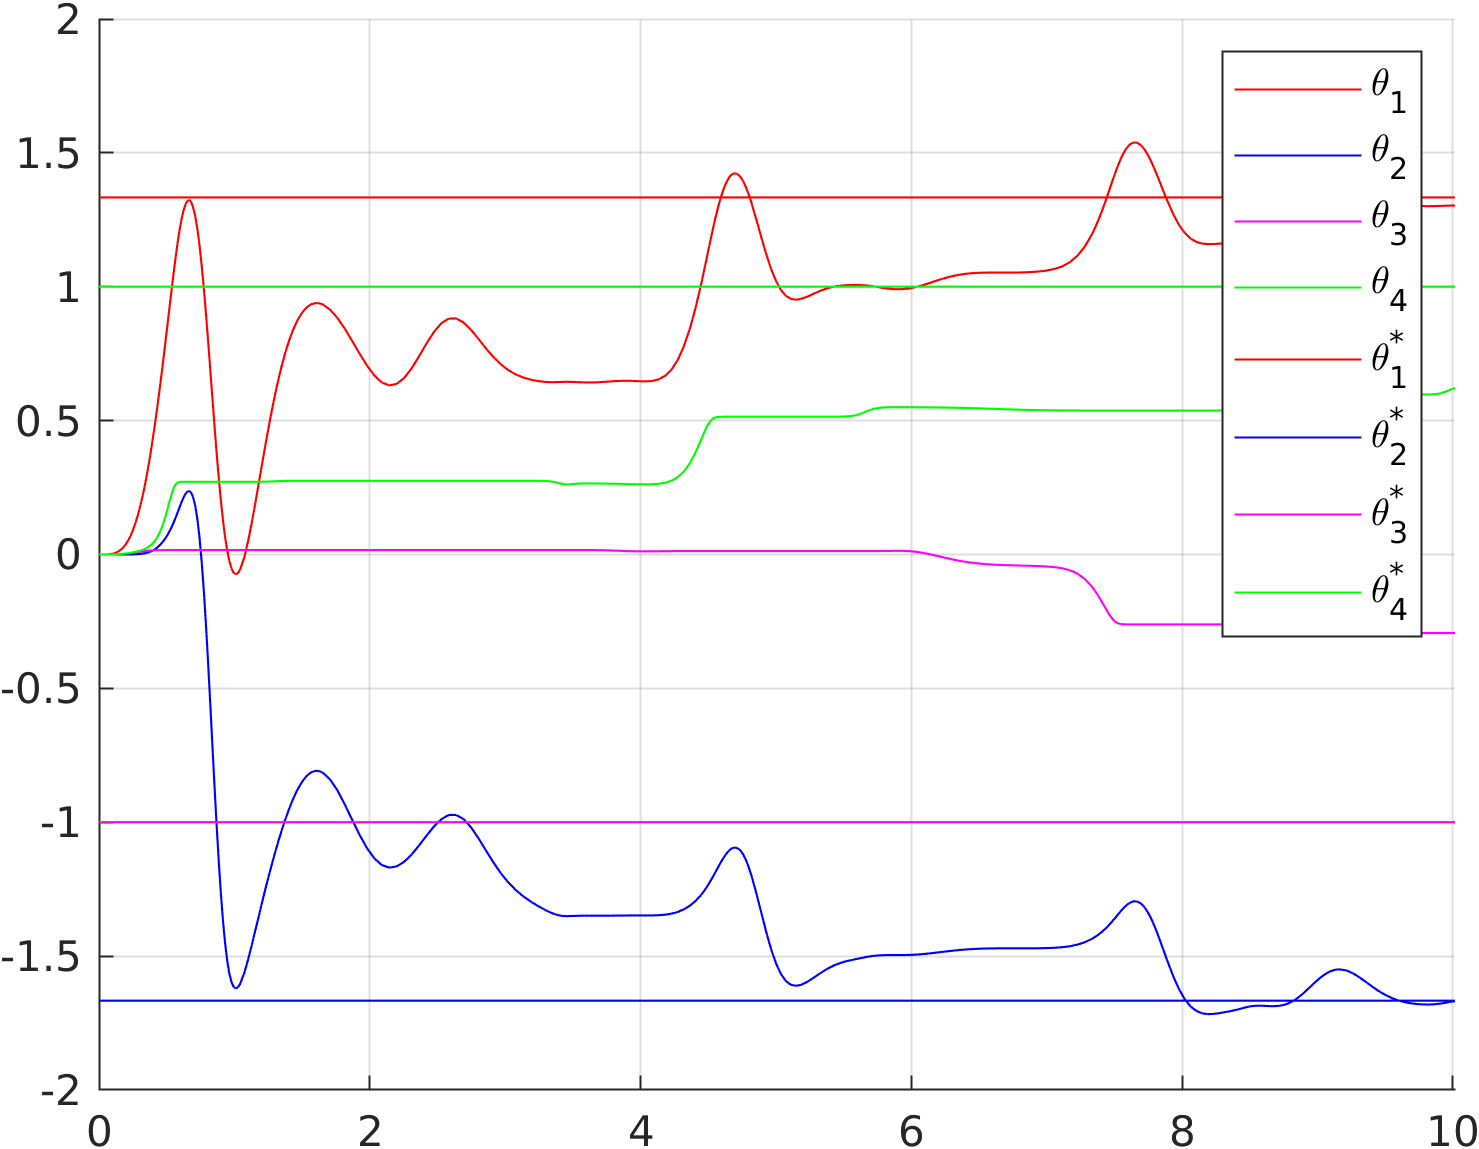
\includegraphics[width=1\textwidth]{Graphics/NonLinearParametersZero1.png}
		\end{subfigure}
		\begin{subfigure}{.45\textwidth}
			\centering
			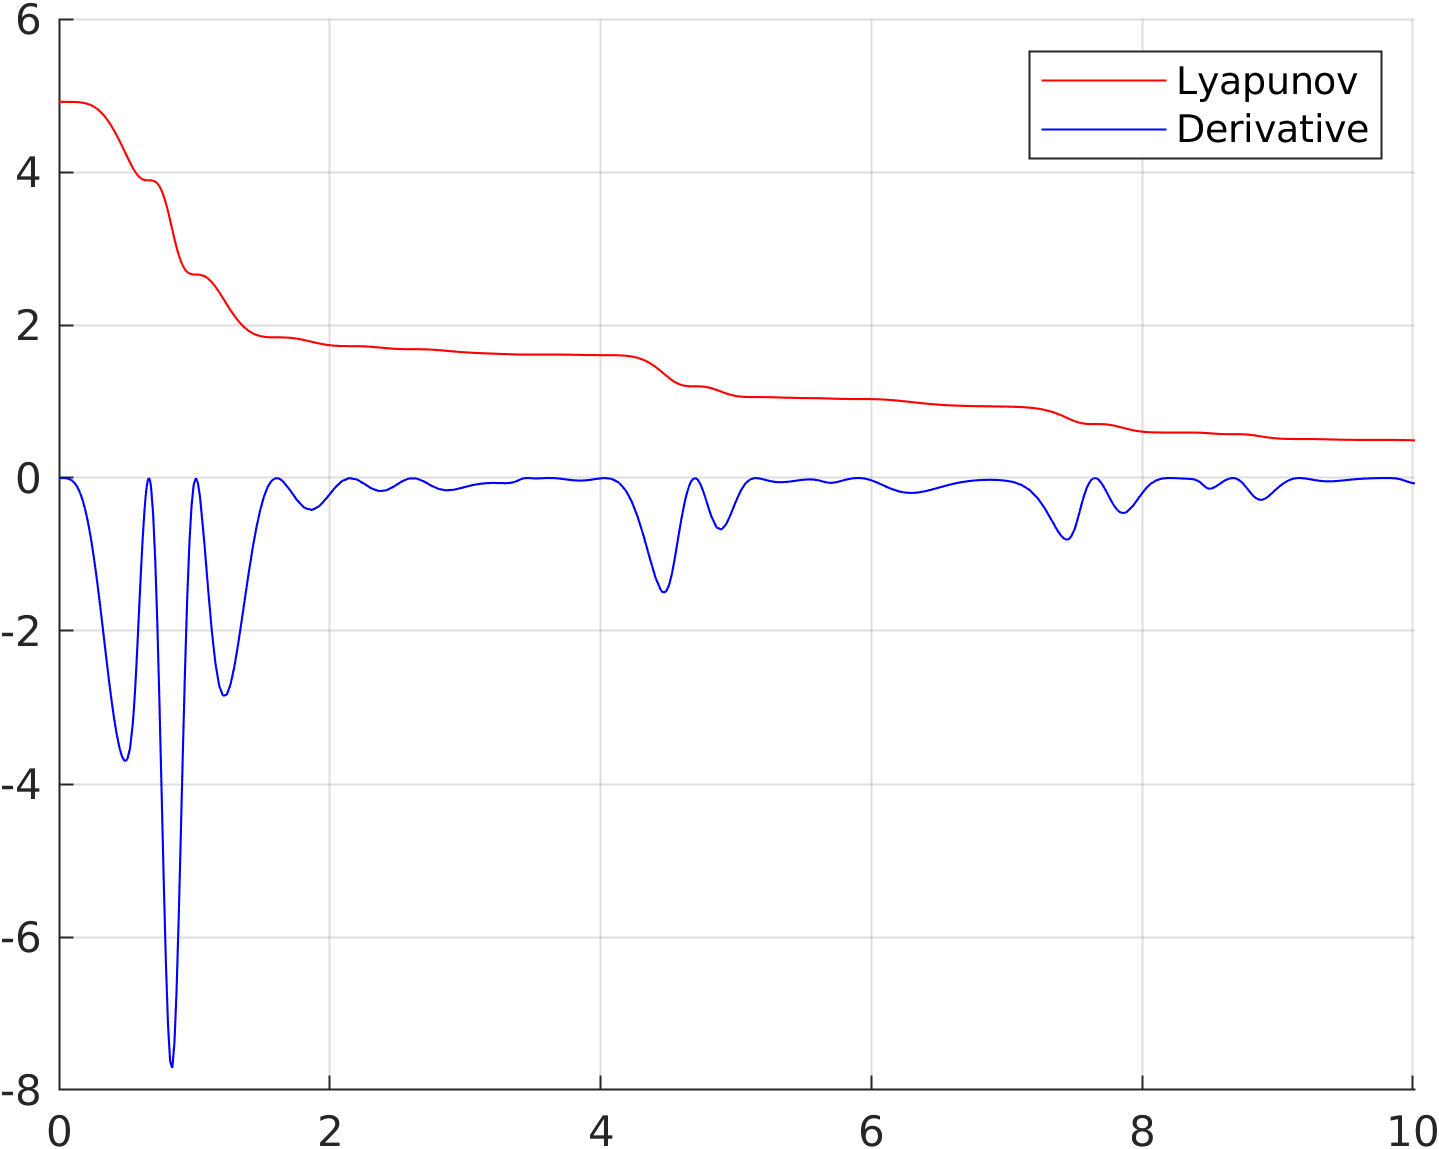
\includegraphics[width=1\textwidth]{Graphics/NonLinearLyapunovZero1.png}
		\end{subfigure}%
		\begin{subfigure}{.45\textwidth}
			\centering
			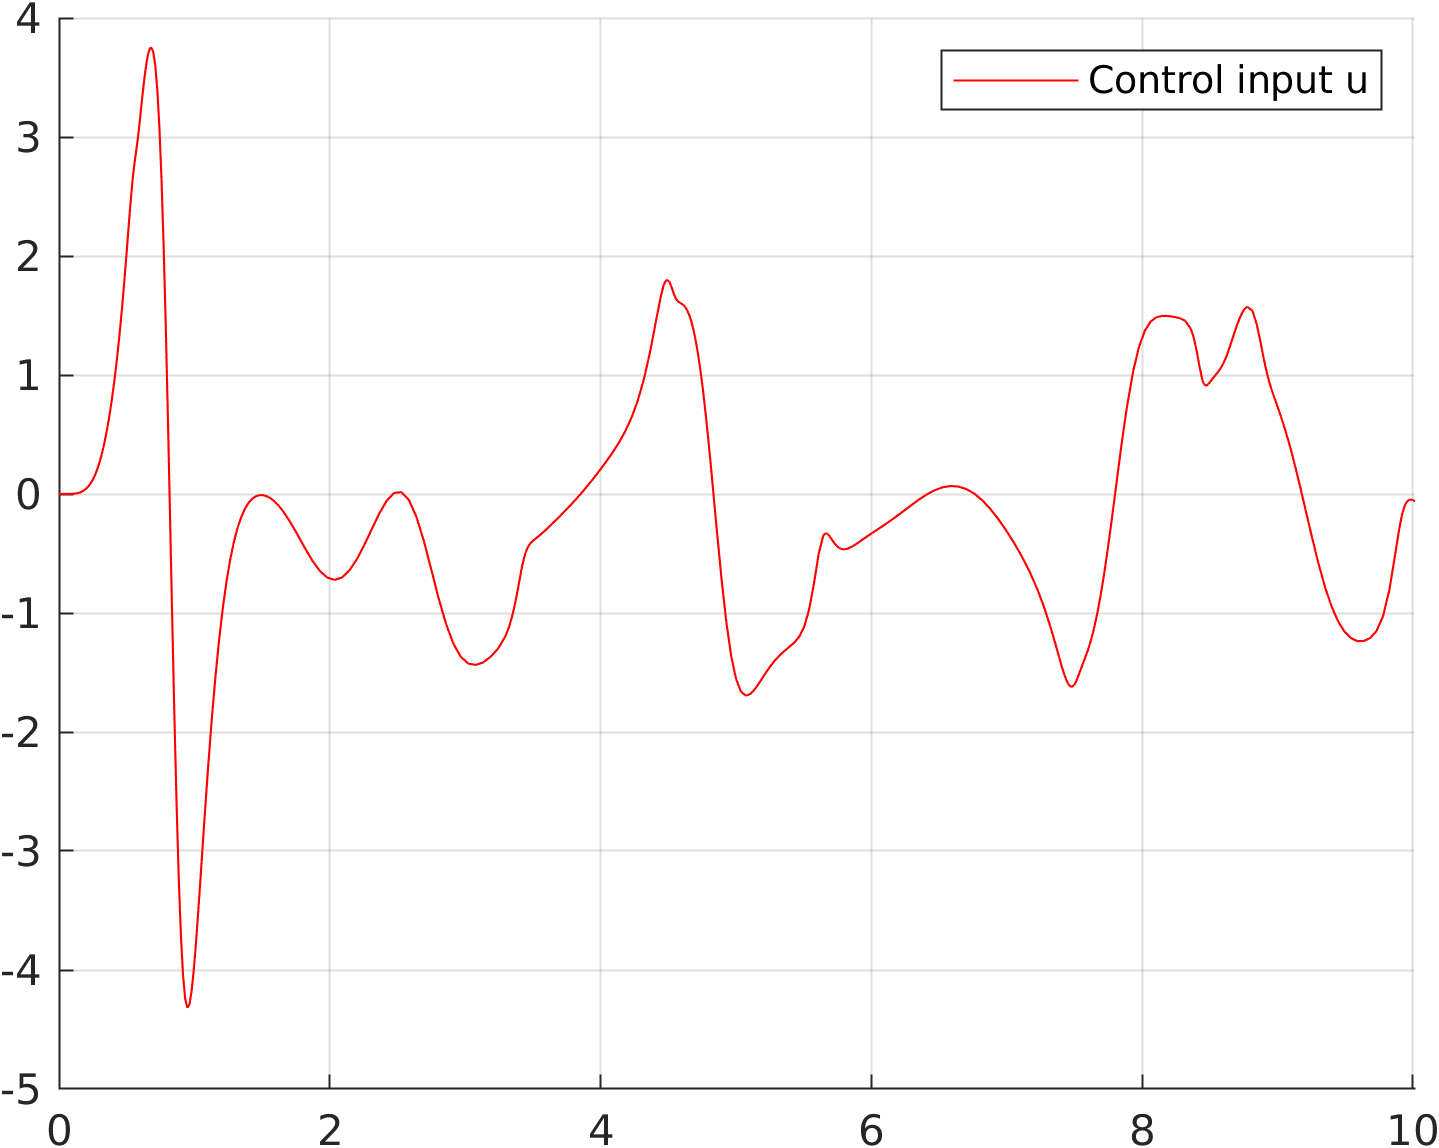
\includegraphics[width=1\textwidth]{Graphics/NonLinearControlZero1.png}
		\end{subfigure}
		\caption{$t \in [0,10]s$, two parameters known to vanish.}
	\end{figure}

	\begin{figure}[H]
		\centering
		\begin{subfigure}{.45\textwidth}
			\centering
			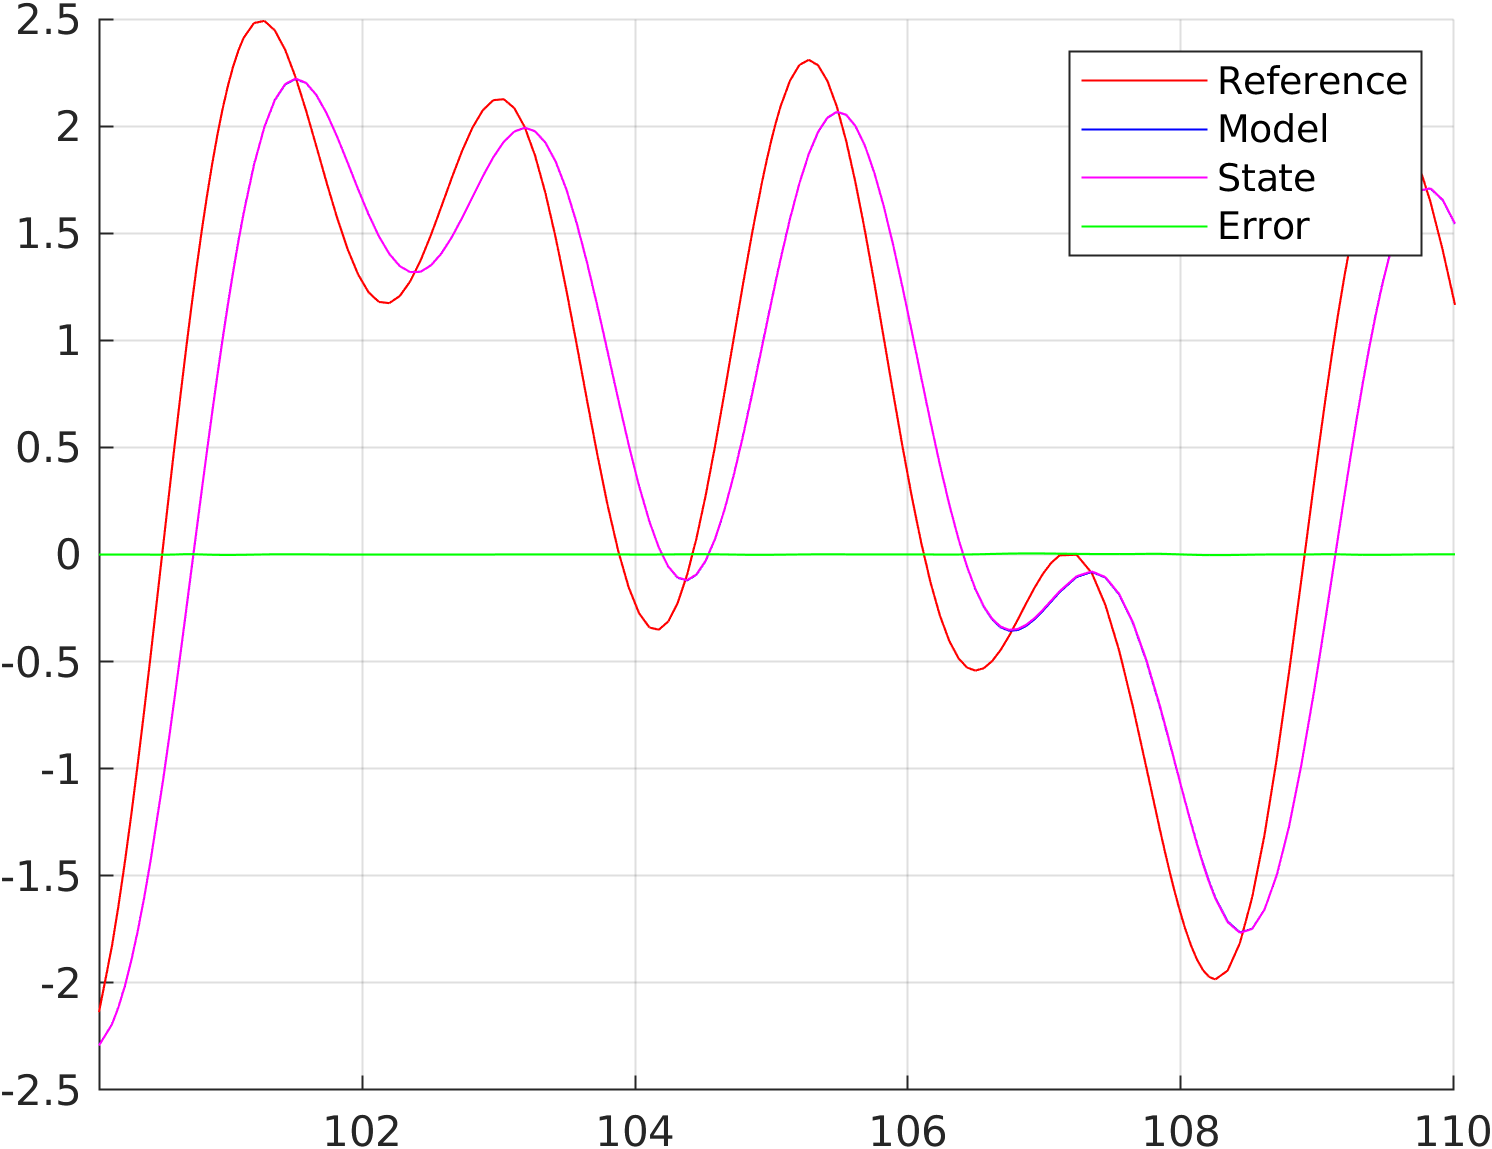
\includegraphics[width=1\textwidth]{Graphics/NonLinearStateZero2.png}
		\end{subfigure}%
		\begin{subfigure}{.45\textwidth}
			\centering
			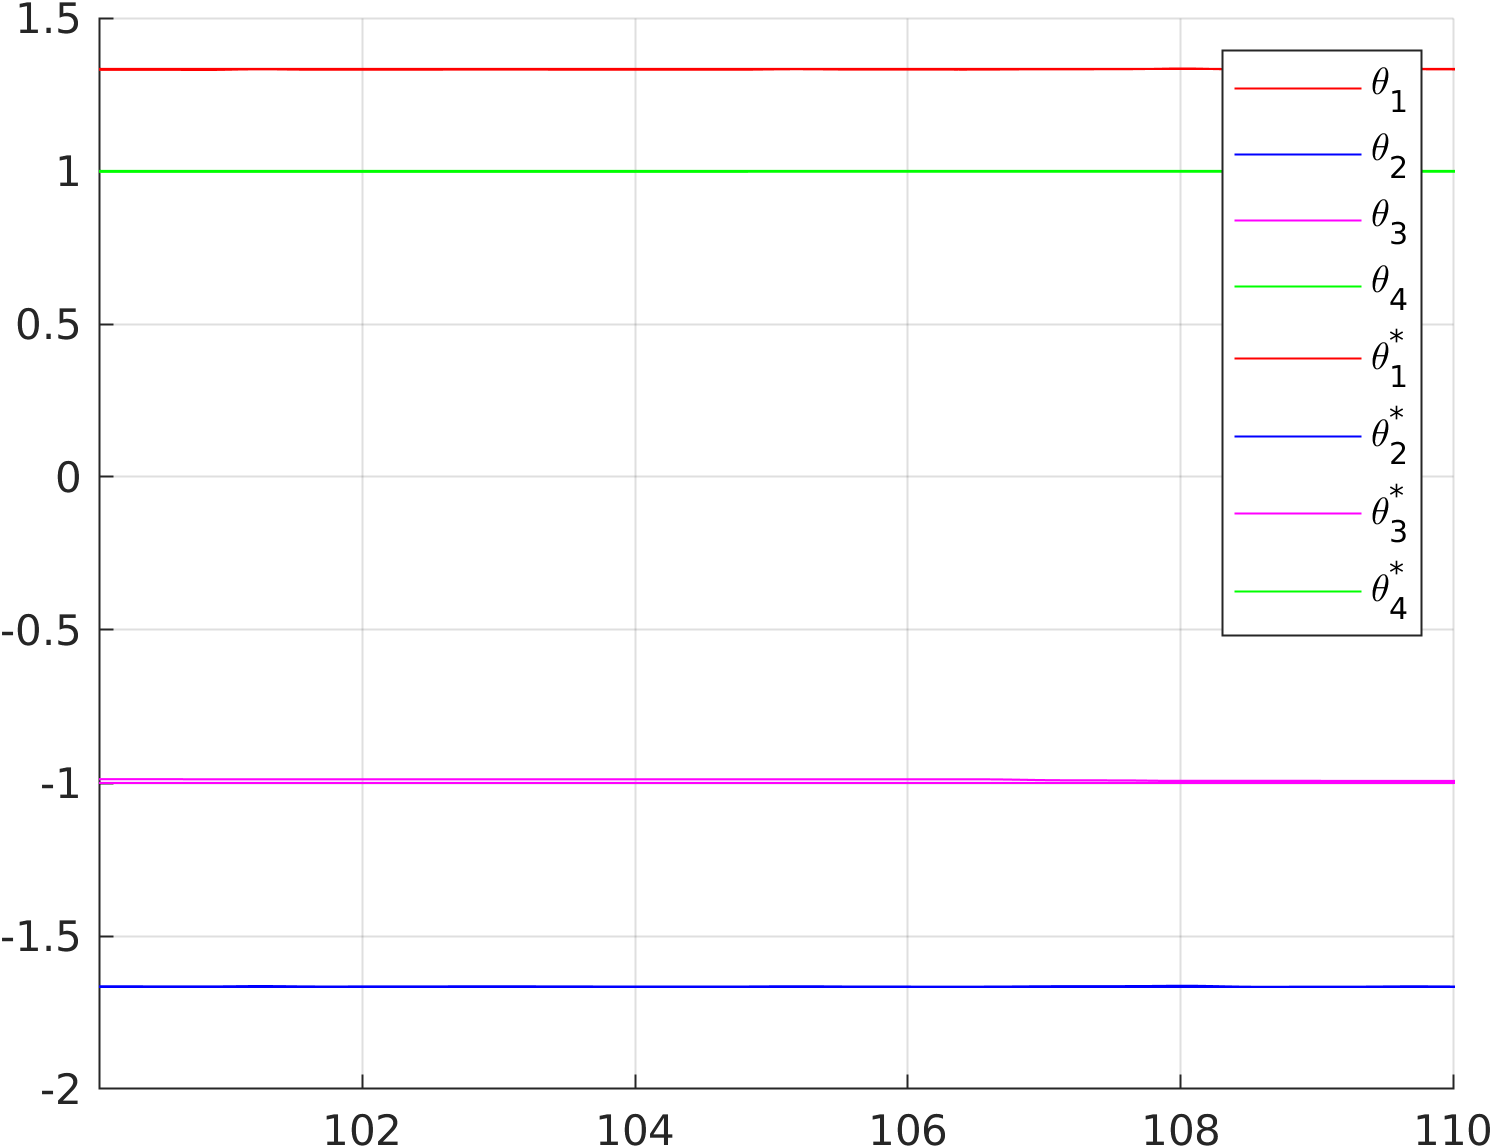
\includegraphics[width=1\textwidth]{Graphics/NonLinearParametersZero2.png}
		\end{subfigure}
		\begin{subfigure}{.45\textwidth}
			\centering
			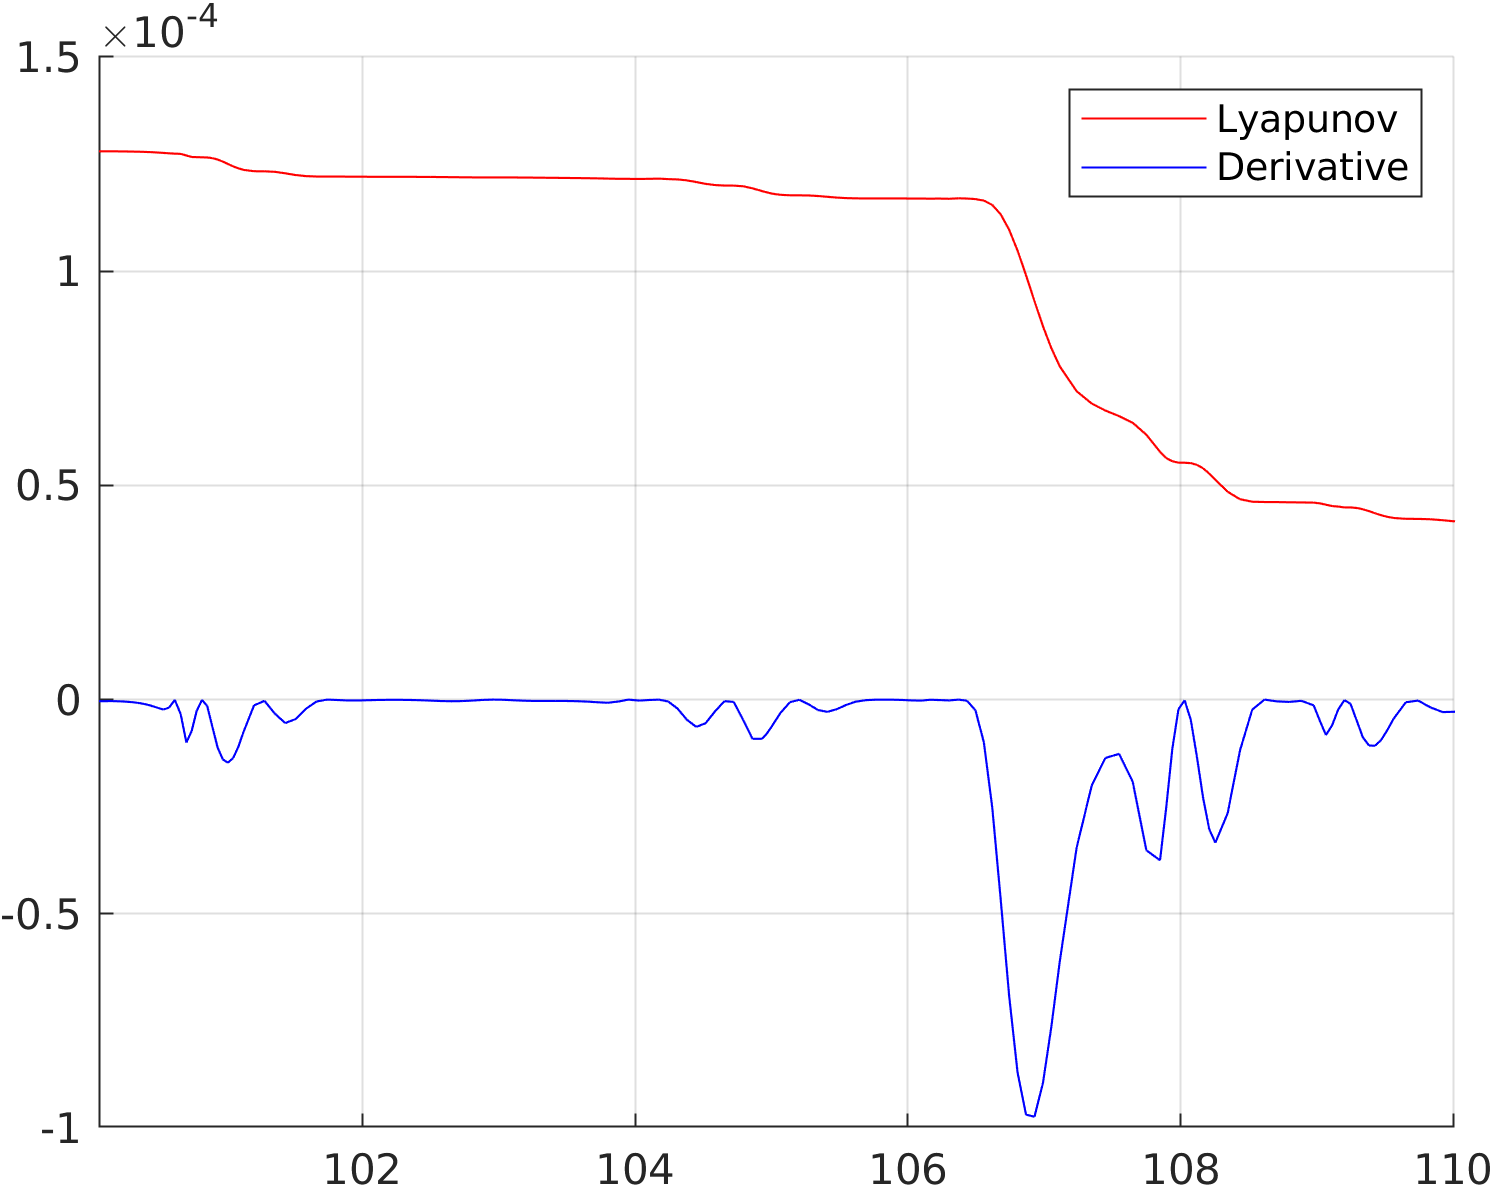
\includegraphics[width=1\textwidth]{Graphics/NonLinearLyapunovZero2.png}
		\end{subfigure}%
		\begin{subfigure}{.45\textwidth}
			\centering
			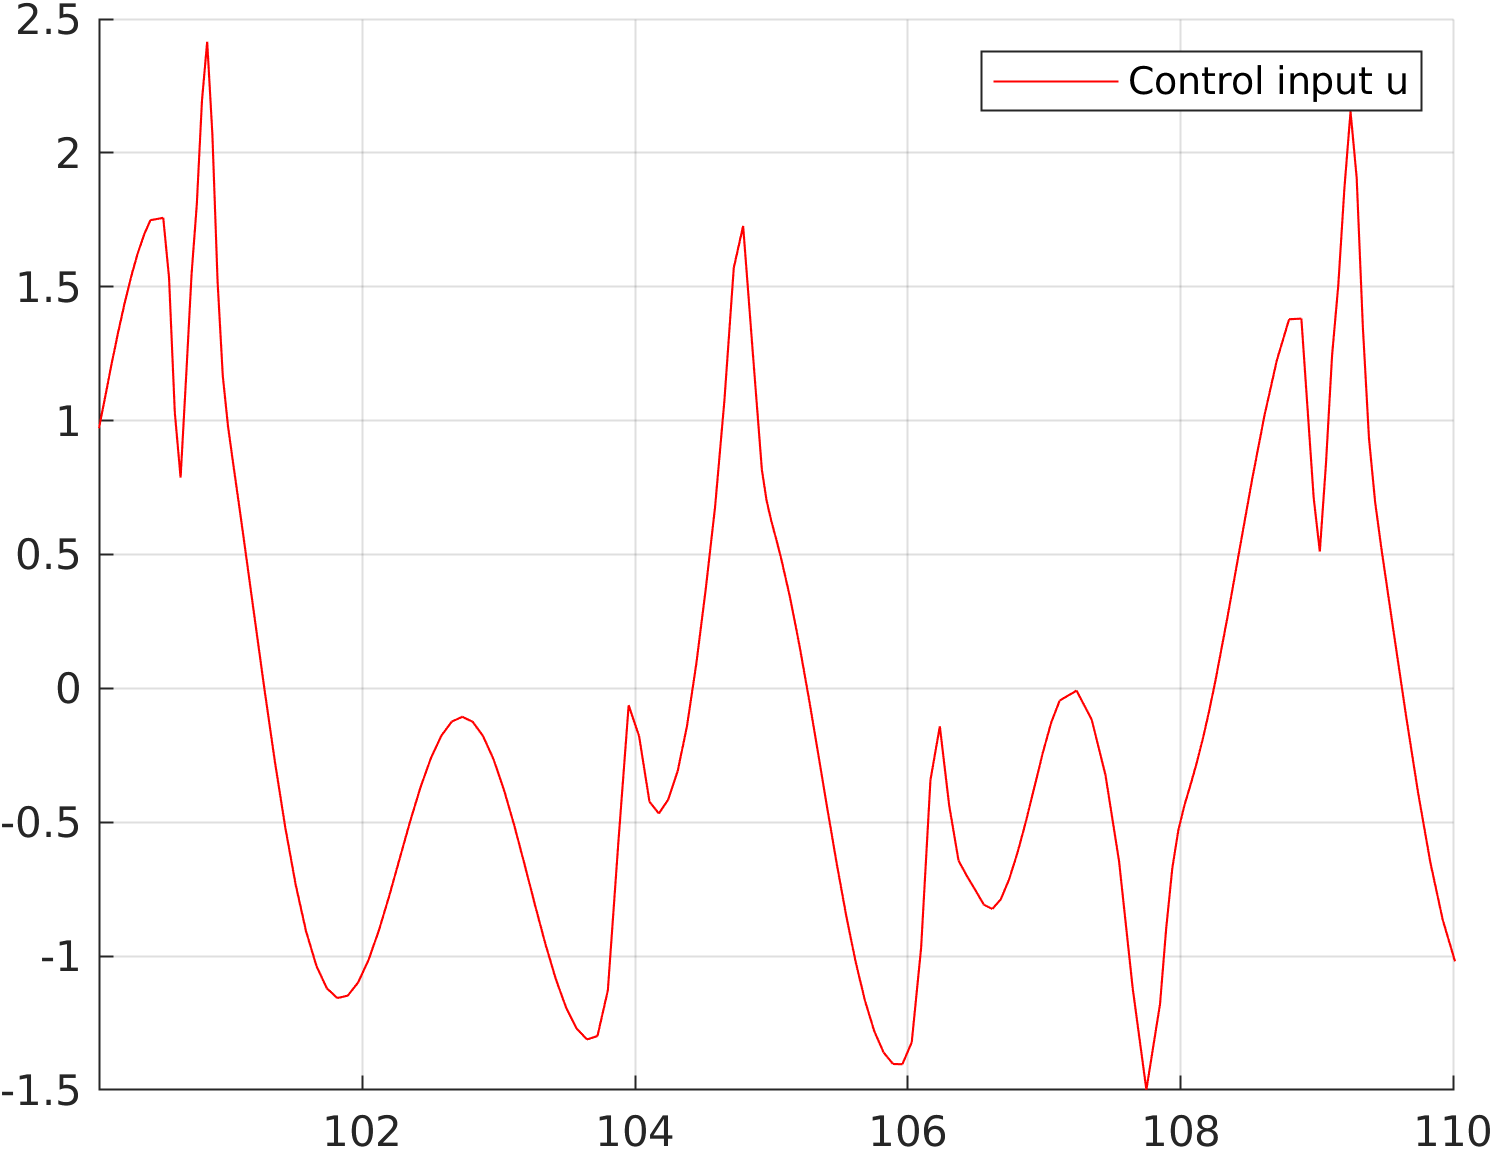
\includegraphics[width=1\textwidth]{Graphics/NonLinearControlZero2.png}
		\end{subfigure}
		\caption{$t \in [100,110]s$, two parameters known to vanish.}
	\end{figure}

	\begin{figure}[H]
		\centering
		\begin{subfigure}{.45\textwidth}
			\centering
			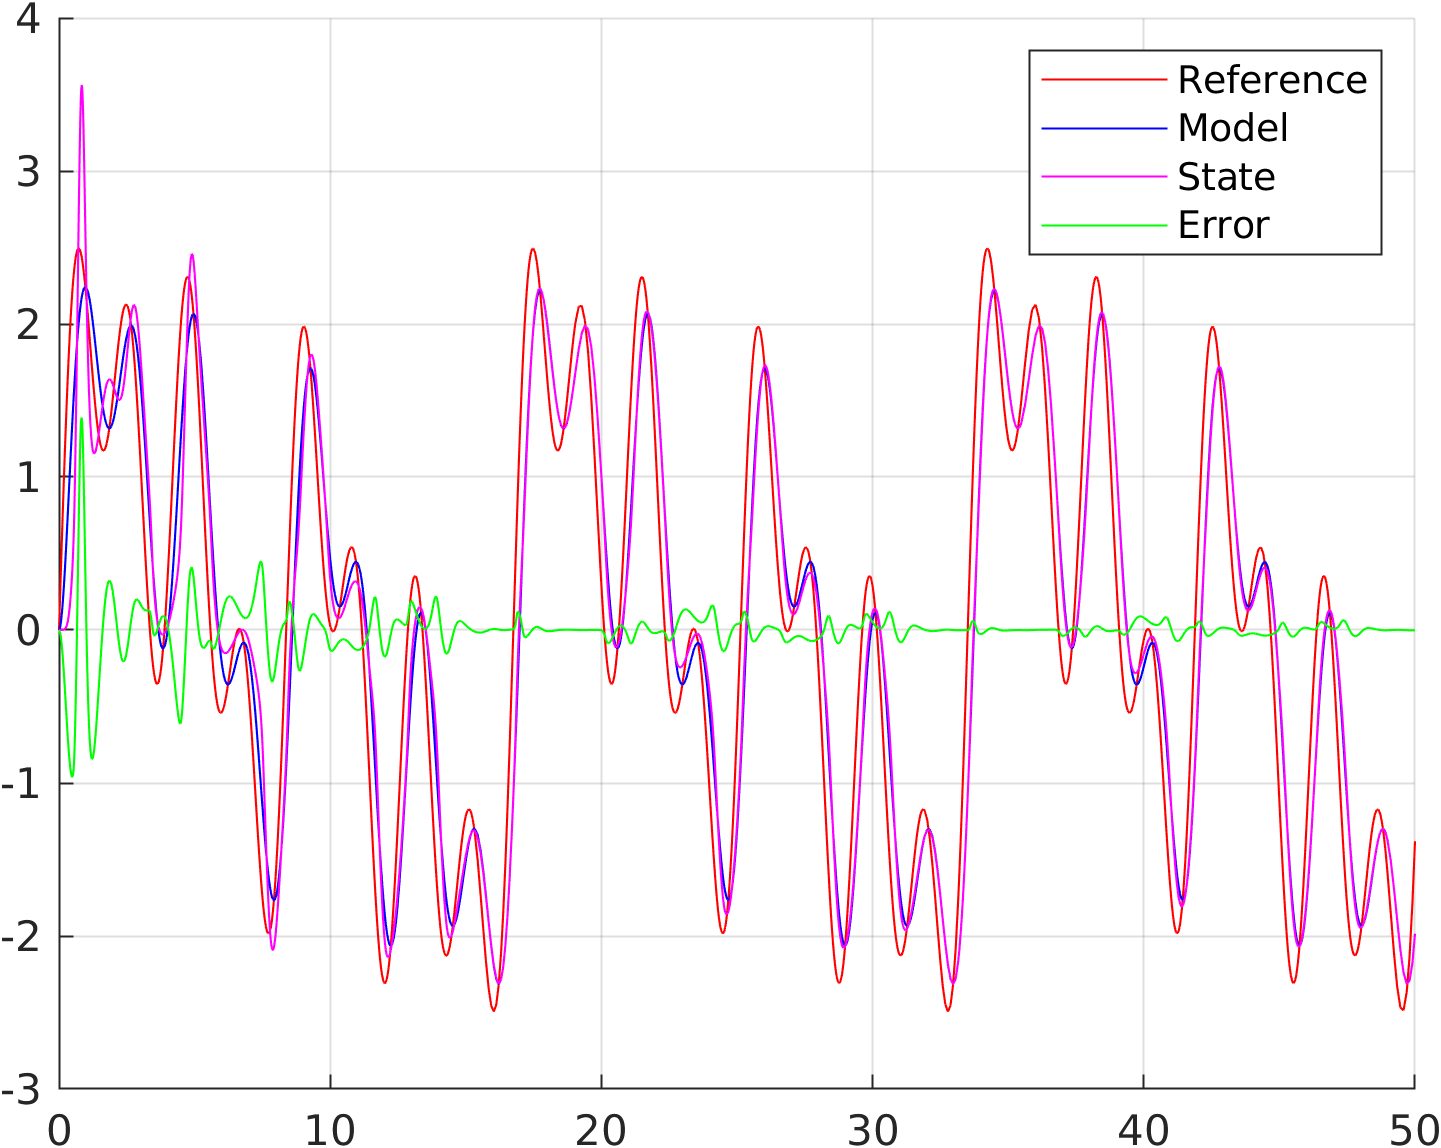
\includegraphics[width=1\textwidth]{Graphics/NonLinearStateZero3.png}
		\end{subfigure}%
		\begin{subfigure}{.45\textwidth}
			\centering
			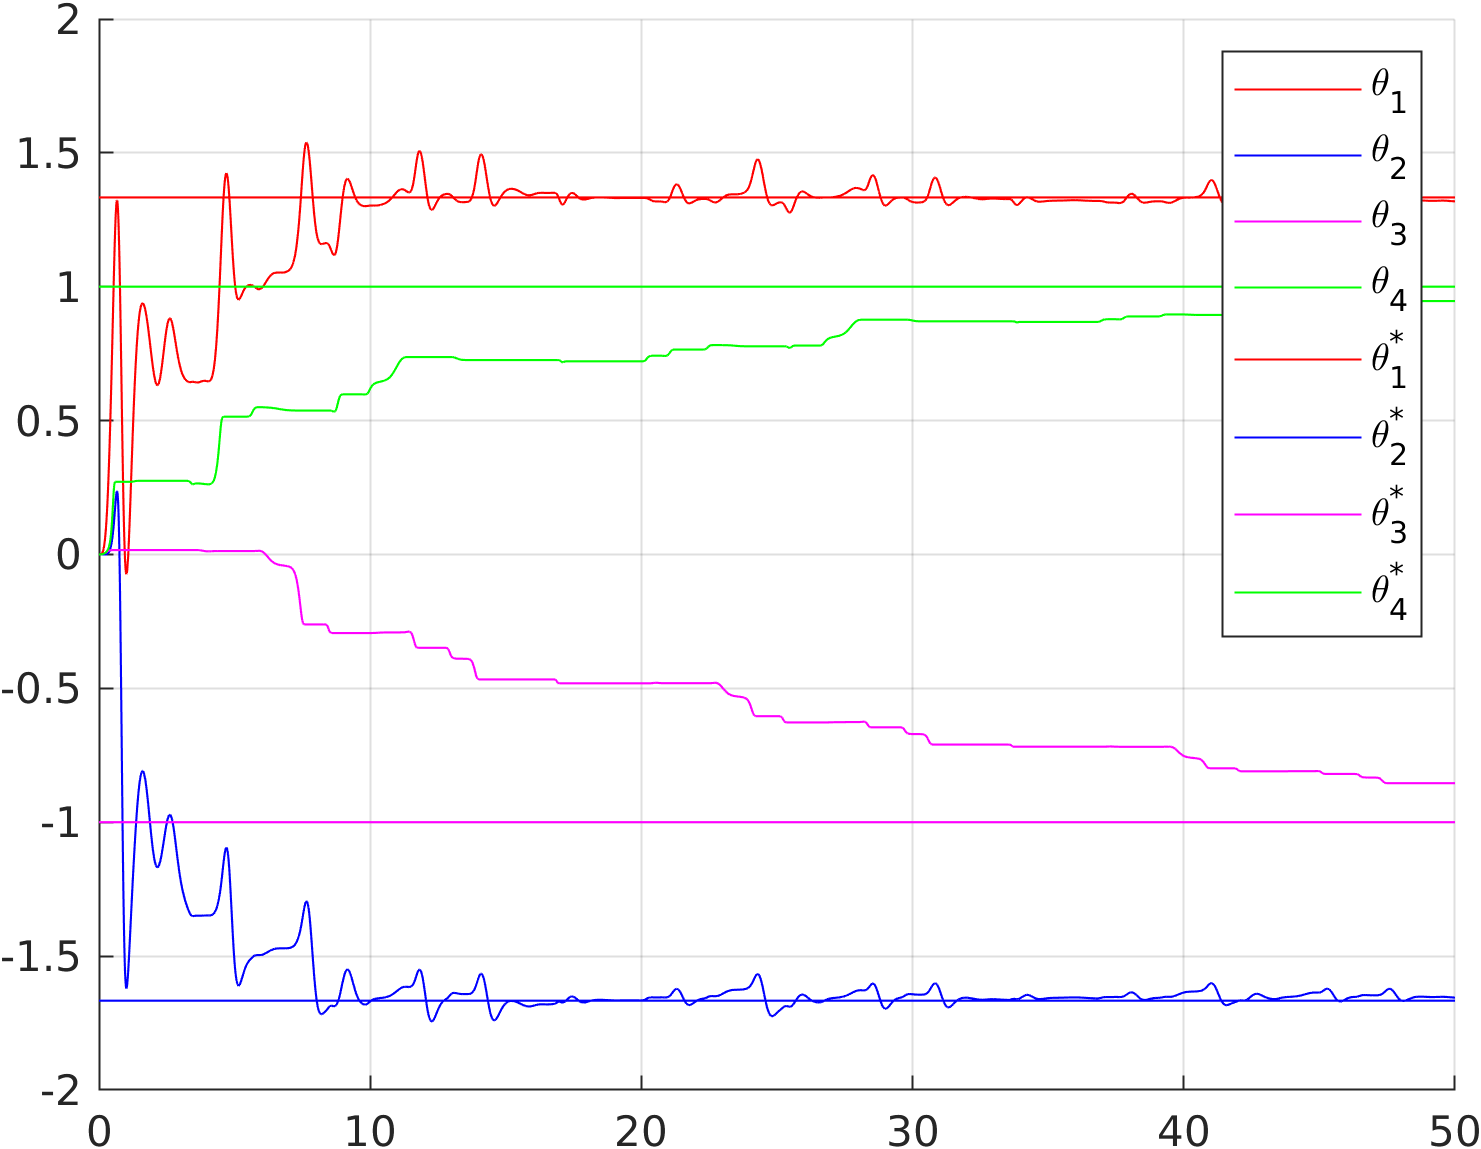
\includegraphics[width=1\textwidth]{Graphics/NonLinearParametersZero3.png}
		\end{subfigure}
		\begin{subfigure}{.45\textwidth}
			\centering
			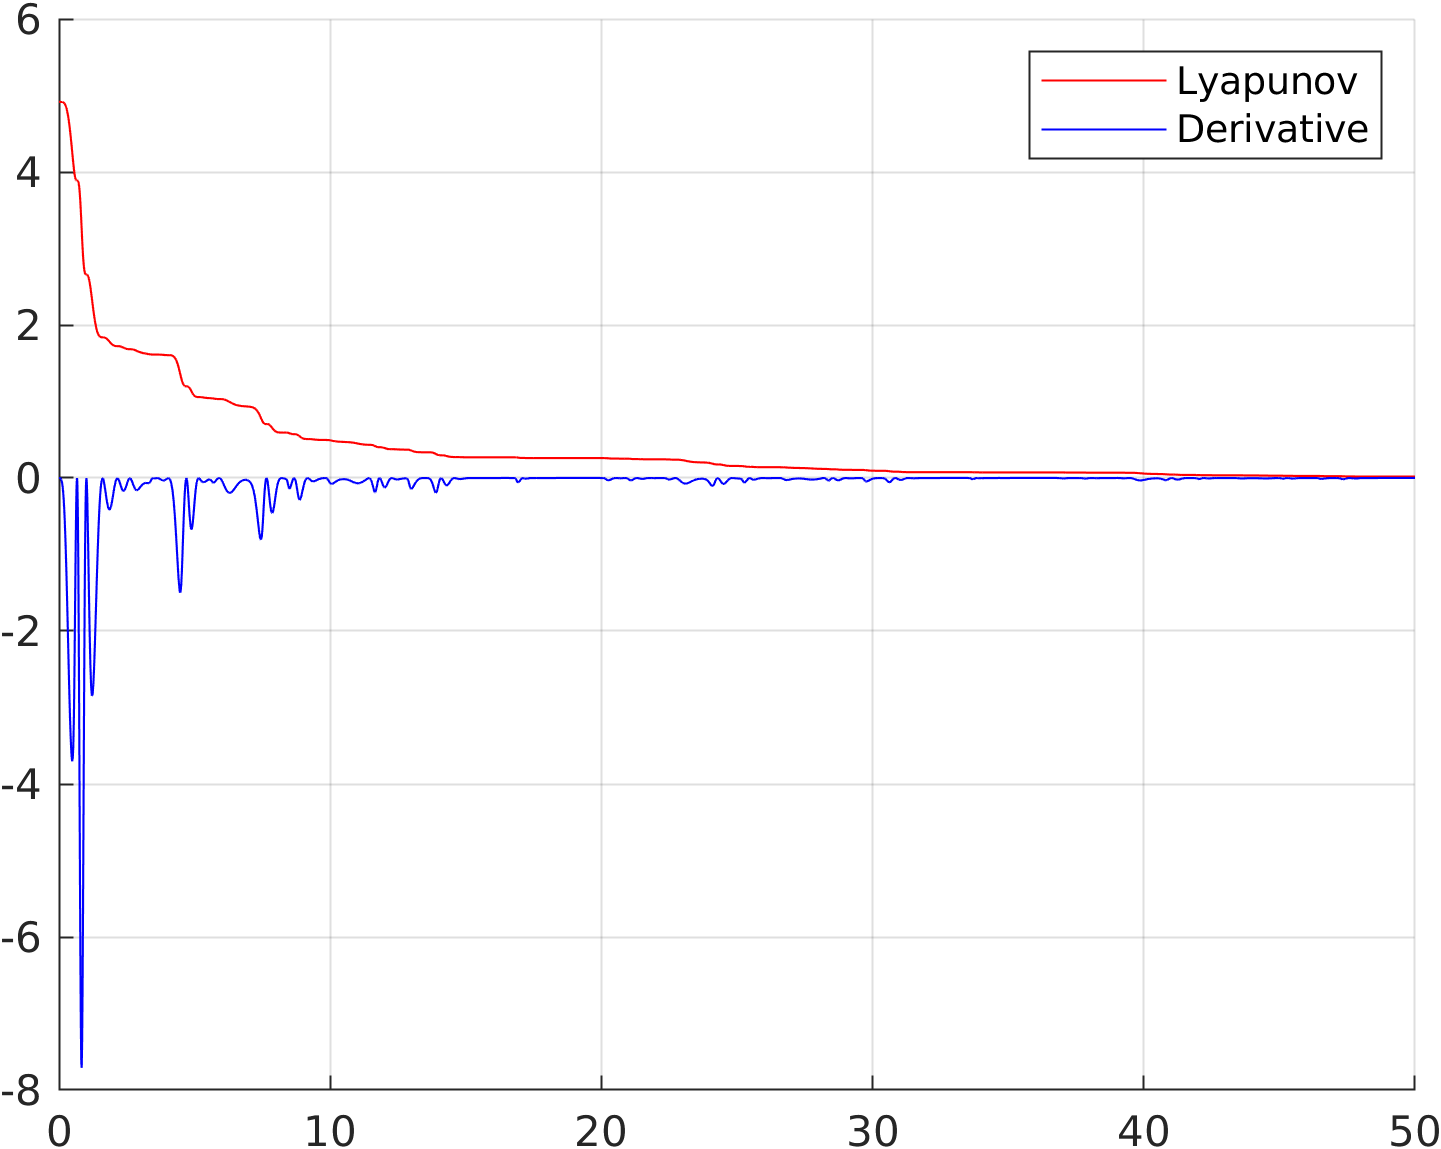
\includegraphics[width=1\textwidth]{Graphics/NonLinearLyapunovZero3.png}
		\end{subfigure}%
		\begin{subfigure}{.45\textwidth}
			\centering
			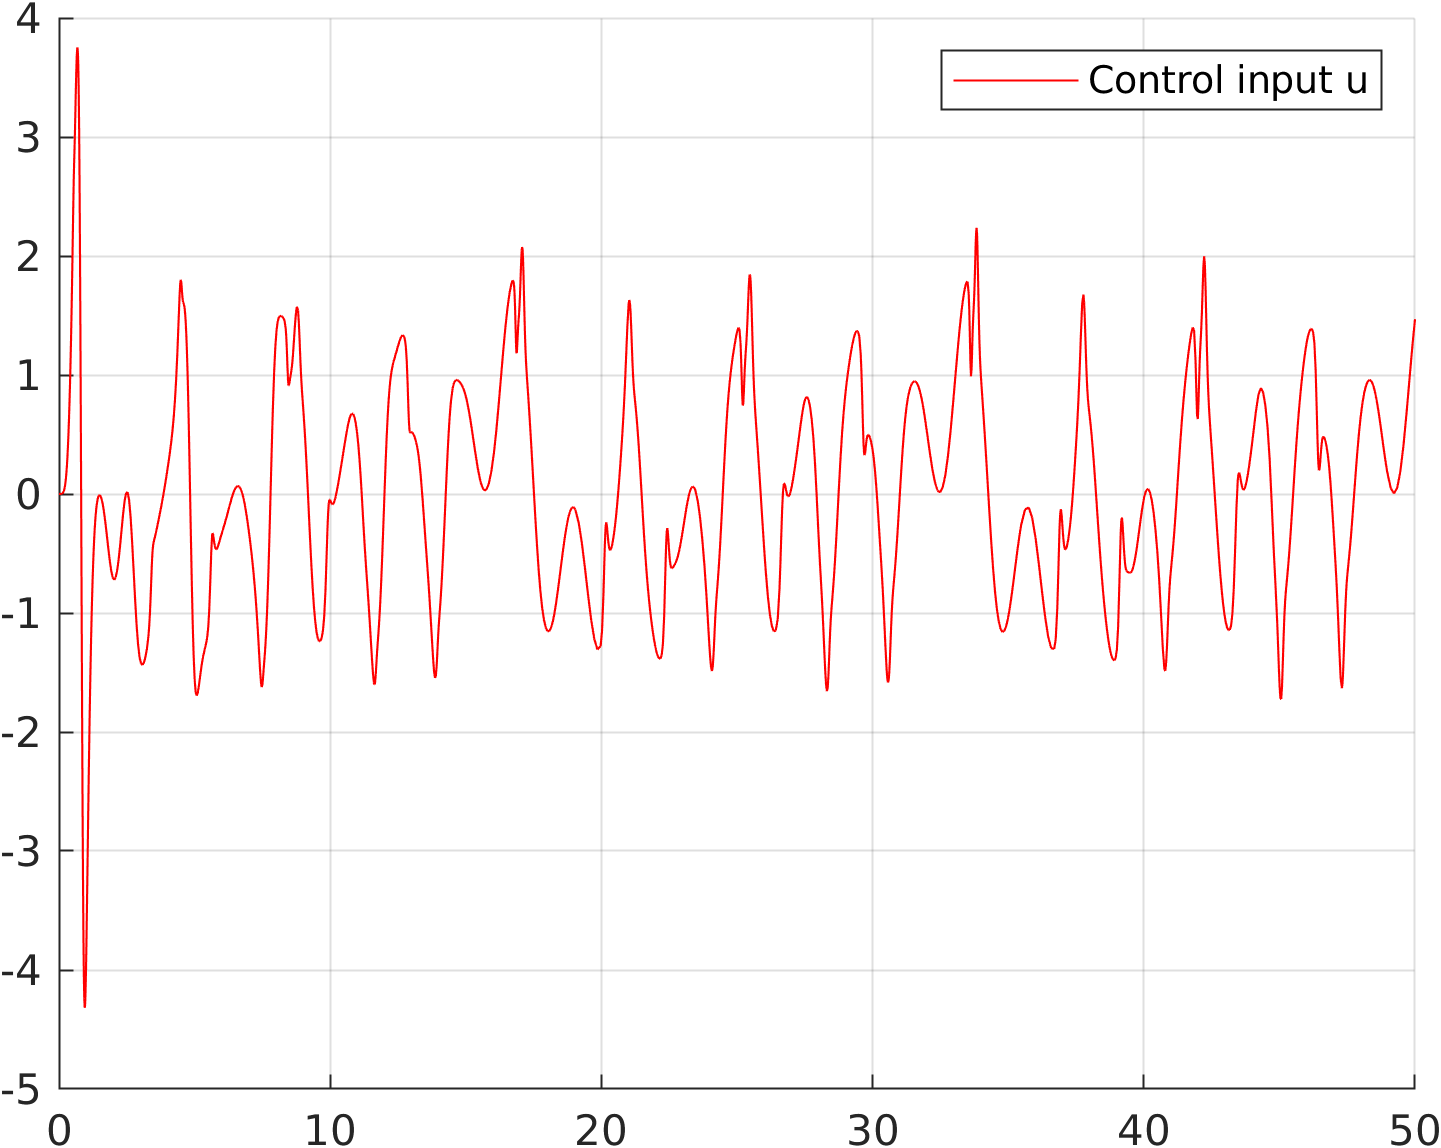
\includegraphics[width=1\textwidth]{Graphics/NonLinearControlZero3.png}
		\end{subfigure}
		\caption{$t \in [0,50]s$, two parameters known to vanish.}
	\end{figure}
	\section*{Problem 2}
	The second part of the homework deals with the problem of parameter convergence of the MRAC-scheme. We already know that the error dynamics
	\begin{equation}
	\label{errordyn}
	e(t) = \frac{1}{k^*}M(s)\Big[ \tilde{\Theta}(t)^T \phi(t)\Big]
	\end{equation}
	is asymptotic stable (this was shown in Theorem 2 of the first part). But we also know that this doesn't imply that $\tilde{\Theta}(t) \to 0\text{, as } t \to \infty$, i.e.$\Theta(t)$ converges to the true parameters $\Theta^*$ or that $\Theta(t)$ converges at all.\\
	In the latter we assume that $\exists t_0:  0 \leq t_0 < \infty \text{ s.t. } e(t_0) \approx 0$ so we can set $e(t) = 0\text{ } \forall t \geq t_0$.\\
	If we now take a look at our adaptive law
	\[ \dot{\Theta}(t) = -\text{sgn}(k_p) \Gamma \phi e\]
	we know that $\dot{\Theta}(t) = 0$ for some finite $t \geq t_0$. Thus $\Theta(t)$ converges in finite time, but we still don't know if it converges to the true parameters $\Theta^*$.\\
	To ensure that $\tilde{\Theta}(t) = 0$ implies that $\Theta(t) \to \Theta^*$, we suggest the following requirement on the regressor $\phi(t)$:
	\begin{equation}
	\label{claim2}
	\int_t^{t+T} \phi(t) \phi(t)^T d\tau \text{ has full rank } \forall t \geq t_0 ,T \in \b{R} 
	\end{equation}
	\\
	To show this we start by looking at equation(\ref{errordyn}) for $t \geq t_0$. If we assume that $k^* \neq 0$ and $k^* \neq \infty$ we obtain that
	\[ 0 = M(s) \Big[ \tilde{\Theta}^T \phi(t)\Big]. \]
	Now we know that $M(s)$ has a nonzero DC-Gain, i.e.
	\[ \lim_{t \to \infty} M(s)y(t) \neq 0\text{ } \forall y(t) \not\equiv 0.\]
	Thus we know that
	\begin{equation}
	\label{regzero}
	0 =  \Big[ \tilde{\Theta}^T \phi(t)\Big] =  \Big[ \phi(t)^T \tilde{\Theta}\Big],
	\end{equation}
	i.e. the two signals must be orthogonal $\forall t \geq t_0$. (Note: The argument of $\tilde{\Theta}^T$, was dropped, because it's constant for $t \geq t_0$).\\
	Now we multiply both sides of equation (\ref{regzero}) with $\phi(t)$ and integrate both sides with respect to $t$ over the interval $[t,t+T]$ and obtain
	\begin{equation}
	\label{rank}
	0 = \int_t^{t+T} \phi(t) \phi(t)^T d\tau \tilde{\Theta}.
	\end{equation}
	$\tilde{\Theta}^T$ can be pulled out of the integral, because its constant.\\
	If the matrix  $\int_t^{t+T} \phi(t) \phi(t)^T d\tau$ has full rank $\forall t\geq t_0$, we know that only the only vector which fulfills equation(\ref{rank}) is the zero vector $\leftrightarrow \text{ } \Theta = \Theta^*$.
        This condition can be checked by finding a variable $\kappa$, such that $\kappa I$ is an lower bound on $\int_t^{t+T} \phi(t) \phi(t)^T d\tau$.\\
        Note that the matrix-claim is equivalent to the claim, that $\phi(t)$ spans the whole $\b{R}^n \forall t \geq t_0$, which makes intuitively sense.\\
        From this claim it directly follows that the reference $r \not\equiv 0$, because otherwise $\phi(t)$ would have a zero-element and would not fulfill (\ref{claim2}).
\end{document}